\documentclass[
% papersize
a4paper,
%fond size
%12pt,
11pt,
%page print style
twoside,
%oneside,
openright]{book}

%for PSTRicks
\usepackage[pdf]{pstricks}
\usepackage[off]{auto-pst-pdf}

%graphics included tikz & pfg
\usepackage{graphicx}
\usepackage{epsfig,epic,eepic}
\usepackage{psfrag}
\usepackage[USenglish,german]{babel}
\usepackage{color,pstricks}
% To allow me to use letters with accent
\usepackage[utf8]{inputenc}

% Fonts
%\usepackage{lmodern}
%from Ruben \usepackage[T1]{fontenc}
\usepackage{times}
%\usepackage[scaled]{helvet}https://www.overleaf.com/project/633c022130834f721b09716d
%\usepackage[sc]{mathpazo} % math fonts for Palatino, see
                          % http://www.tug.dk/FontCatalogue/palatino/
%\usepackage{palatino}

% Math packages
\usepackage{amsmath,amssymb,amsfonts,amsthm}
\usepackage{url}
\usepackage[ruled,noline]{algorithm2e}
% More compact lists
\usepackage{paralist}
% Fullpage
\usepackage[in,headings]{fullpage}
% But then adapt spacing
\usepackage{setspace}
\setstretch{1.3}

%for nice tables
\usepackage{multirow}
%\usepackage{booktabs}
\usepackage{tikz}
% \usepackage{ctable}
% \usepackage[transparency]{xcolor} % Enable transparency support
%for nice item lists
\usepackage{paralist}

%usepackage comment for block comments
\usepackage{comment}

%nice symbols to draw arrow (yes) and -(no)
\usepackage{pifont}
\newcommand{\yes}{\checkmark}
\newcommand{\no}{\textendash}

%sub-picture numbering
%\usepackage{subcaption}
\usepackage{subfigure}

\usepackage[right]{eurosym}
\usepackage{pdflscape}
% svg
\usepackage{svg}


%annotate TODO stuff
\usepackage[colorinlistoftodos, textwidth=4cm, shadow]{todonotes}
\usepackage{lscape}

%pseudocode package
\usepackage{pseudocode}
%add code
\usepackage{listings}
%add floating fig
\usepackage{placeins}


%add greek
\usepackage{textalpha}
%to insert some clickable links
\usepackage{hyperref}
\definecolor{darkblue}{rgb}{0,0,.5}
\definecolor{black}{rgb}{0,0,0}
\hypersetup{colorlinks=true, breaklinks=true, citecolor=black, linkcolor=black, menucolor=black, urlcolor=black}

% \setlength{\oddsidemargin}{-0.3cm}
% \setlength{\evensidemargin}{-0.3cm}
% \setlength{\textwidth}{16cm}
% \setlength{\topmargin}{-0.8cm}
% \setlength{\textheight}{23.0cm}

% use some common definitions
\newcommand{\pref}[1]{Part~\ref{#1}}
\newcommand{\cref}[1]{Chapter~\ref{#1}}
\newcommand{\sref}[1]{Section~\ref{#1}}
\newcommand{\aref}[1]{Appendix~\ref{#1}}
\newcommand{\fref}[1]{Figure~\ref{#1}}
\newcommand{\tref}[1]{Table~\ref{#1}}
\newcommand{\eref}[1]{(\ref{#1})}

% More convenient sometimes
\newcommand{\ie}{i.\@e.\@ }
\newcommand{\eg}{e.\@g.\@ }

\newcommand{\us}{\,$\mu$s\xspace}

%add empty page macro
\newcommand{\blankpage}{
\newpage
\thispagestyle{empty}
\mbox{}
\newpage
}

% Some math definitions

%\newcommand{\indic}{1\hspace{-2.5mm}{1}}
%\newcommand{\indic}{\boldsymbol{1}}
\newcommand{\indic}[1]{1_{\{#1\}}}
\newcommand{\erfc}{\mathrm{erfc}}
\newcommand{\abs}[1]{\left\lvert #1 \right\rvert}
\newcommand{\lp}[1]{\left( #1 \right)}
\newcommand{\lb}[1]{\left\lbrack #1 \right\rbrack}
\newcommand{\lc}[1]{\left\lbrace #1 \right\rbrace}
\newcommand{\erf}[1]{\mathrm{erf}\lp{#1}}
\newtheorem{definition}{Definition}
\newtheorem{lemma}{Lemma}
\newtheorem{theorem}{Theorem}

\newcommand{\calI}{\mathcal I}
\newcommand{\calN}{\mathcal N}
\newcommand{\calP}{\mathcal P}
\newcommand{\calX}{\mathcal X}
\newcommand{\calC}{\mathcal C}

% Paper specific notation
\def\su{^{(u)}}
\def\s0{^{(0)}}
%
\def\Xr{X^{(r)}}
\def\Xt{X^{(t)}}
%
\def\Ns{N_{\textrm{s}}}
\def\Na{N_{\textrm{a}}}
%
\def\tacq{t_{\textrm{acq}}}
\def\ttx{t_{\textrm{tx}}}
\def\tfail{t_{\textrm{fail}}}
\def\tdrop{t_{\textrm{drop}}}
%
\def\tprop{t_{\textrm{prop}}}
\def\tpreamble{t_{\textrm{preamble}}}
\def\tdata{t_{\textrm{DATA}}}
\def\tack{t_{\textrm{ACK}}}
\def\tsigidle{t_{\textrm{SIGIDLE}}}
\def\tmaxbackoff{t_{\textrm{max backoff}}}
\def\tsendtimer{t_{\textrm{send timer}}}
\def\tidletimer{t_{\textrm{idle timer}}}
\def\tbackoff{t_{\textrm{backoff}}}
%
\def\SD{S_{\textrm{D}}}
\def\SI{S_{\textrm{I}}}
%
\def\Pacq{p_{\textrm{acq}}}
\def\Pfail{p_{\textrm{fail}}}
\def\Pbusy{P_{\textrm{busy}}}
\def\Pmd{P_{\textrm{MD}}}
\def\Pfa{P_{\textrm{FACQ}}}
%
\def\td{t_{\textrm{D}}}
\def\ti{t_{\textrm{I}}}
\def\Np{N_{\textrm{p}}}


\newcommand{\mand} {\mathrm{\;  and \; }}
\newcommand{\mfor} {\mathrm{\;  for \;  }}
\def\Ints{\mathbb{Z}}
\def\P{\mathbb{P}}
\def\E{\mathbb{E}}
\def\be{\begin{equation}}
\def\ee{\end{equation}}
\def\ben{\[}
\def\een{\]}
\def\bearn{\begin{eqnarray*}}
\def\eearn{\end{eqnarray*}}
\def\bear{\begin{eqnarray}}
\def\eear{\end{eqnarray}}
\def\barr{\begin{array}}
\def\earr{\end{array}}
\def\bel{\be \barr{l}}% equation array adjusted left, numbered
\def\eel{\earr\ee}
\def\beln{\ben \barr{l}}% equation array adjusted left, no number
\def\eeln{\earr\een}\def\be{\begin{equation}}
\def\ee{\end{equation}}
\def\ben{\[}
\def\een{\]}
\def\bearn{\begin{eqnarray*}}
\def\eearn{\end{eqnarray*}}
\def\bear{\begin{eqnarray}}
\def\eear{\end{eqnarray}}
\def\barr{\begin{array}}
\def\earr{\end{array}}
\def\bel{\be \barr{l}}% equation array adjusted left, numbered
\def\eel{\earr\ee}
\def\beln{\ben \barr{l}}% equation array adjusted left, no number
\def\eeln{\earr\een}


% Style headings + headers and footers

% Modify header and footers
\usepackage{fancyhdr}
\pagestyle{fancy}
\fancyhf{}
\renewcommand{\chaptermark}[1]{
  \markboth{\thechapter.\ #1}{}
%  \markboth{#1}{}
}
\renewcommand{\sectionmark}[1]{
%  \markboth{\thechapter.\ #1}{}
  \markright{#1}
}

% \fancyhead[LE]{\normalfont\sffamily\thepage}
% \fancyhead[RE]{\normalfont\sffamily\leftmark}
% \fancyhead[LO]{\normalfont\sffamily\rightmark}
% \fancyhead[RO]{\normalfont\sffamily\thepage}
\fancyhead[LE]{\normalfont\thepage}
\fancyhead[RE]{\normalfont\leftmark}
\fancyhead[LO]{\normalfont\rightmark}
\fancyhead[RO]{\normalfont\thepage}

% Modify the fonts for the chapters, section, sub... and paragraphs
\usepackage{titlesec}

\titleformat{\chapter}[display]
%{\normalfont\Huge\sffamily}
{\normalfont\Huge}
{\filleft{\textbf{\LARGE{\chaptername} {\thechapter}}}}{1em}{\filleft\textbf}

\titleformat{\section}
{\normalfont\Large}
{\filright{\textbf{\thesection}}}{1em}{\filright\textbf}

\titleformat{\subsection}
{\normalfont\normalsize}
{\filright{\textbf{\thesubsection}}}{1.3em}{\filright\textbf}

\titleformat{\subsubsection}
{\normalfont\normalsize}
{}{0em}{\filright\textbf}

\titleformat{\paragraph}[runin]
{\normalfont\normalsize}
{}{0em}{\filright\textbf}

% Do it for theorems,... too
%\theoremstyle{definition}
%\newtheorem{define}{\textbf\normalfont\normalsize\sffamily{Definition}}[chapter]
%\theoremstyle{plain}
%\newtheorem{theorem}{\textbf\normalfont\normalsize\sffamily{Theorem}}[chapter]
%\newtheorem{lem}{\textbf\normalfont\normalsize\sffamily{Lemma}}[chapter]


% The larger it is, the less willing LaTeX is to split footnotes
\interfootnotelinepenalty=10000


% Removing master, slows down the compilation
\includeonly{
	title,
	abstract,
	acknowledgments,
	paper-collaborators,
	eid,
	chapter-1_introduction,
	chapter-2_measurement_tools,
	chapter-3_analysis_and_optimization,
	chapter-4_conclusion,
	appendix,
}


% BEGINN of DOCUMENT
\begin{document}

\setlength{\headheight}{13.6pt}

%TITLE PAGE

% Titeseite

\begin{titlepage}
  \begin{center}
	  
    %\mbox{}

    %\vspace{1cm}

	\centering
	
\includegraphics[width=3cm]{figures/tub.pdf}\\
	\vspace{0.8em}
	\LARGE 

	\textsc{Technische Universit\"at Berlin}

    \vspace{1cm}

    \sffamily \LARGE \textbf{My new Master thesitests titel comes here}

    \vspace{1.5cm}





    \normalsize vorgelegt von

    \vspace{.1cm}

    \large Alex the student (Dipl.-Ing.)

    \vspace{.8cm}

  %  von der Fakult�t IV - Elektrotechnik und Informatik der Technischen Universit�t Berlin


    \normalsize von der Fakult\"{a}t IV -- Elektrotechnik und Informatik\\
    %\vspace{.1cm}
    \normalsize der Technischen Universit\"{a}t Berlin\\
    %\vspace{.1cm}
    \normalsize zur Erlangung des akademischen Grades\\
    %\vspace{.1cm}
    \large \textsc{Diplom der Ingenieurwissenschaften (Dipl.-Ing.)}\\
    %\vspace{.1cm}
    \normalsize genemigte Diplomarbeit\\

    \vspace{1cm}

    \large \textbf{Diplomausschuss:}

    \vspace{.2cm}

		\begin{tabular}{rl}
		Pr\"ufer der Diplomarbeit:	& Prof. Dr.-Ing. XYZ, TU-Berlin\\
						& Dr.-Ing. XYZ, TU-Berlin\\
		\end{tabular}\\

    \vspace{2cm}
    \large Tag der wissenschaftlichen Verteidigung: 11.01.2013\\
    \vspace{0.5cm}
    \large Berlin 2013\\

  \end{center}
\end{titlepage}


\selectlanguage{USenglish}

%ABSTRACT_EN
\frontmatter \pagestyle{plain}
\setcounter{page}{1}
%\addcontentsline{toc}{chapter}{Resume}
\chapter*{Abstract}
\label{chap:abstract}

%
\textit Abstract .....




%ACKNOWLAGEMENTS
\addcontentsline{toc}{chapter}{Acknowledgments}
\chapter*{Acknowledgments}
\label{chap:ack}

%Acknowledgements for all the helping hands

\section*{}
At first, I want to thank ...





%PUBLICATIONS & COLLABORATORS
% \chapter*{Pre-Published Papers}
% \label{chap:prepublished_papers}

% Parts of this thesis are based on the following peer-reviewed papers that have already been published. All my collaborators are among my co-authors.
% %

% %%%%%%%%%%%%%%%%%%%%%%%%%%%%%%%%%%%%%
% %%%%%%%%%%%%%%%%%%%%%%%%%%%%%%%%%%%%%
% %%%%%%%%%%%%   SECTION   %%%%%%%%%%%%
% %%%%%%%%%%%%%%%%%%%%%%%%%%%%%%%%%%%%%
% %%%%%%%%%%%%%%%%%%%%%%%%%%%%%%%%%%%%%
% \section*{Journals}
% \begin{list}{}
% 	{\leftmargin=2em \itemindent=-2em}
% 	\item 
% 		\textsc{Alex the student, Adam, Eve}: ``Challenges in Online Learning Platforms'', EURASTUD Journal on European Student Teaching,  2008, P. 1\hbox{-}10.
% 	%\item
% \end{list}
% \smallskip

% %%%%%%%%%%%%%%%%%%%%%%%%%%%%%%%%%%%%%
% %%%%%%%%%%%%%%%%%%%%%%%%%%%%%%%%%%%%%
% %%%%%%%%%%%%   SECTION   %%%%%%%%%%%%
% %%%%%%%%%%%%%%%%%%%%%%%%%%%%%%%%%%%%%
% %%%%%%%%%%%%%%%%%%%%%%%%%%%%%%%%%%%%%
% \section*{International Conferences}
% \begin{list}{}
% 	{\leftmargin=2em \itemindent=-2em}
% 	\item 
% 		\textsc{Alex the student}: ``Practical Online Learning Tools'', in 21st International Student Teaching Conference (ISTC), 2012, P. 1\hbox{-}7.
% 	%\item
% \end{list}
% \smallskip

% %%%%%%%%%%%%%%%%%%%%%%%%%%%%%%%%%%%%%
% %%%%%%%%%%%%%%%%%%%%%%%%%%%%%%%%%%%%%
% %%%%%%%%%%%%   SECTION   %%%%%%%%%%%%
% %%%%%%%%%%%%%%%%%%%%%%%%%%%%%%%%%%%%%
% %%%%%%%%%%%%%%%%%%%%%%%%%%%%%%%%%%%%%
% \section*{Workshops}
% \begin{list}{}
% 	{\leftmargin=2em \itemindent=-2em}
% 	\item 
% 	\textsc{Alex the student, Eve} : ``Online Learning Monitoring and Debugging through Measurement Visualization'', in the 4th IEEE International Workshop on Hot Topics in Online Learning (IEEE HotOnLe'12), 2012, P. 1\hbox{-}6.
% 	%\item
% \end{list}
% \smallskip


% %%%%%%%%%%%%%%%%%%%%%%%%%%%%%%%%%%%%%
% %%%%%%%%%%%%%%%%%%%%%%%%%%%%%%%%%%%%%
% %%%%%%%%%%%%   SECTION   %%%%%%%%%%%%
% %%%%%%%%%%%%%%%%%%%%%%%%%%%%%%%%%%%%%
% %%%%%%%%%%%%%%%%%%%%%%%%%%%%%%%%%%%%%
% %\section*{Posters and Demos}
% %\begin{list}{}
% %	{\leftmargin=2em \itemindent=-2em}
% %	\item 
% %	\textsc{Alex the student, Adam}: ``OnTeMoS: Online Teacher Monitoring System'', in the 3rd International Workshop on Online Learning Approaches, Experimental Evaluation and Characterization, New York, NY, USA, 20013, P. 101\hbox{-}102.
% 	%\item
% %\end{list}

%EIDESSTATTLICHE ERKLAERUNG
%SELBSTAENDIGKEITSERKLAERUNG
\newcommand{\theauthor}{Elham Aref}
\pagestyle{empty}

\vspace*{\stretch{1}}
\setlength{\parindent}{0in}
%Ich versichere an Eides statt, dass ich diese Diplomarbeit selbst\"andig verfasst und nur die angegebenen Quellen und Hilfsmittel verwendet habe.
%
%Alle w\"ortlich oder inhaltlich \"ubernommenen Stellen habe ich als solche gekennzeichnet.
%
%Die vorliegende Arbeit wurde weder in der vorliegenden noch einer modifizierten Fassung einer dritten, in- oder ausl\"andischen Fakult\"at als Pr\"ufungsleistung, oder zum Erlangen eines akademischen Grades vorgelegt.

I hereby confirm this thesis been written on my own and only used the aids indicated.
The current work was not submitted to a third, domestic or foreign faculty as an examination, neither in the present nor in a modified version, or to obtain an academic degree.

\vspace{1cm}

\begin{flushright}
	\begin{tabular}{p{2cm}p{6cm}}
		\hline
		2023.2.14  & \theauthor
		\smallskip
	\end{tabular}
\end{flushright}


% %INSERT EMPTY PAGE
% \blankpage

%TOC PAGE
\tableofcontents
%MAIN CONTENT
\mainmatter \pagestyle{fancy}
%\pagestyle{headings}

\chapter{Introduction}
\label{chap:introduction}

General Introduction


\section{Problem Statement}
\label{sec:intro:probstatement}

\section{Contributions}
\label{sec:intro:contrib}


\begin{itemize}
\item {\bf Measurements}
\item{\bf Evaluation Tools}

\end{itemize}

\chapter{Measurement Tools}
\label{chap:Measurement Tools}

\section{Data collection Setup}
\label{sec:Measurement Tools:Data collection Setup}

The data used in the analysis of this thesis, was collected in an unsupervised environment over the course of several days~\ref{sec:data_set}. The experiment involved an APU2E4 access point~\cite{PC_Engines_apu2e4}.

The AP is  equipped with an Atheros~AR9287 wireless chip~\cite{atheros-ar9287}, "The Atheros~AR9287 is a wireless chipset that is compatible with the ath9k Linux kernel driver. It supports IEEE 802.11n wireless networking standards and operates in both the 2.4~GHz and 5~GHz frequency bands. The chipset is known for its reliability, low power consumption, and high throughput. It is commonly used in wireless routers and access points, and it is capable of supporting multiple antennas for improved performance. The ath9k driver provides stable and efficient support for the AR9287~chipset in Linux-based operating systems."

The stations, that were connected to the access point (AP) in the wireless network under observation were a diverse. These stations were located in various positions and orientations, with some being stationary while others were mobile. As the measurements were taken in real-life scenarios, the stationary devices were not static and occasionally moved around, causing variations in signal strength and quality. Mobile devices were moving more frequently, which is observable from signal strength value~\ref{RSSI}.

The movement of the stations may have been caused by the users themselves, as they moved around with their devices, or by other environmental factors, such as interference from other wireless devices or obstacles in the environment. These variations in the signal strength value and quality can impact the transmission rates and the overall performance of the wireless network. Further details will be presented in chapter-3~\ref{chap:Analysis and Optimization}.

Therefore, it is essential to consider the mobility and dynamic nature of the stations when analyzing the wireless network's performance. A detailed description of the environment, including the physical layout and the location of the stations, can provide valuable insights into the performance of the network and help optimize the wireless communication system. Chapter-3 will provide additional information~\ref{chap:Analysis and Optimization}.
The data transmission of each station present on a particular day is depicted in the Figure~\ref{fig:plot_22_population}. For more information on the environment in which the measurements were taken, please refer to the Appendix~\ref{sec:data_set}. 

\begin{landscape}

\begin{figure}[htbp]
  \centering
    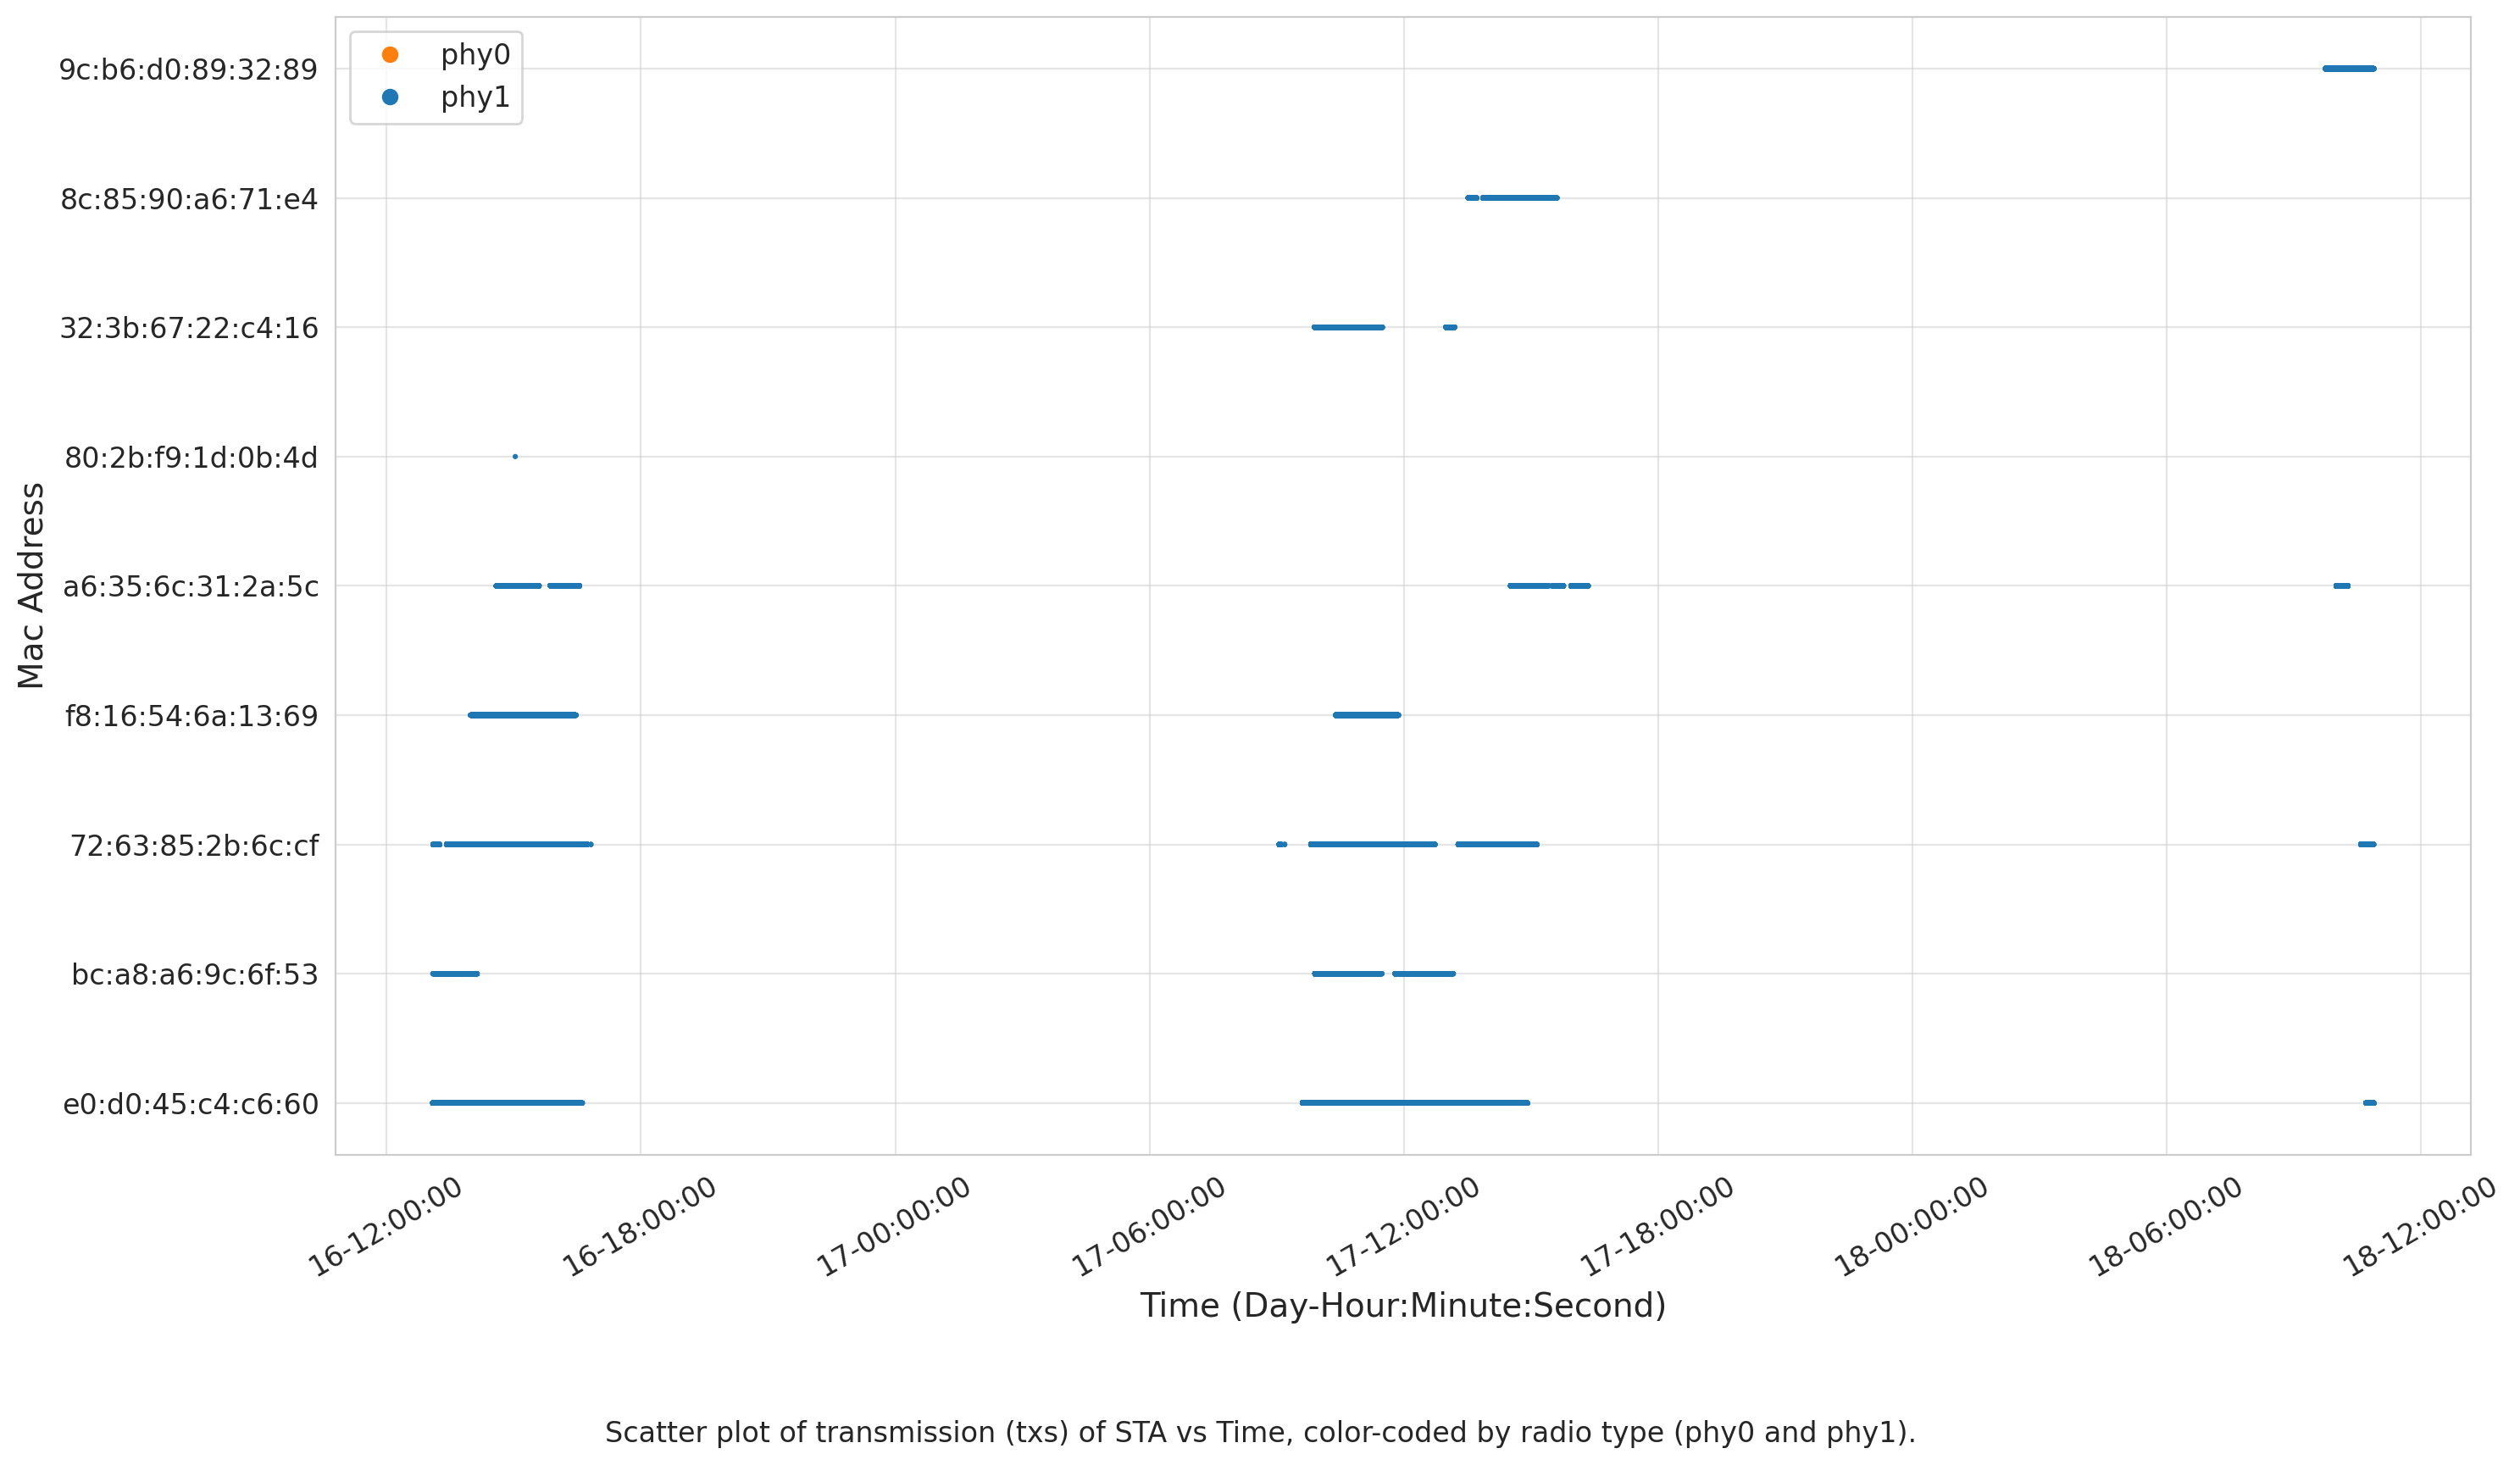
\includegraphics[width=\textwidth, height=\textheight, keepaspectratio]{figures/plots/22.png}
  \caption[Stations' Transmission Over Time]{Scatter plot of transmission (txs) of STA vs Time, color-coded by radio type (phy~0, phy~1, and others).}
  \label{fig:plot_22_population}
\end{figure}
\end{landscape}

\section{Format of Monitoring Information}
\label{sec:Measurement Tools:Format of Monitoring Information}

The trace files fetched from the Linux kernel Minstrel-HT contain detailed information about network events. The first eight lines of a log file serve as the header of a monitoring map for the rest of the event lines. Lines nine through fifty-one are related to groups, and a precise description of these groups is available in reference~\ref{sec:intro:wifiratecontrol:Group creation}. An example of header lines are shown in Figure~\ref{fig:plot_csv1}

After the header lines, each line of the report indicates an event related to a station being connected to the access point, with the MAC address of the station being specified. These events have a nanosecond resolution UNIX timestamp, providing precise information about the exact timing of each event. Figure~\ref{fig:plot_csv2} is a sample of a trace file.

It is important to note that the information contained in these trace files can be used to analyze network performance and identify potential issues. By carefully examining the events recorded in the trace files, researchers can gain valuable insights into the behavior of the network and take steps to optimize its performance.


\begin{figure}[htbp]
  \centering
  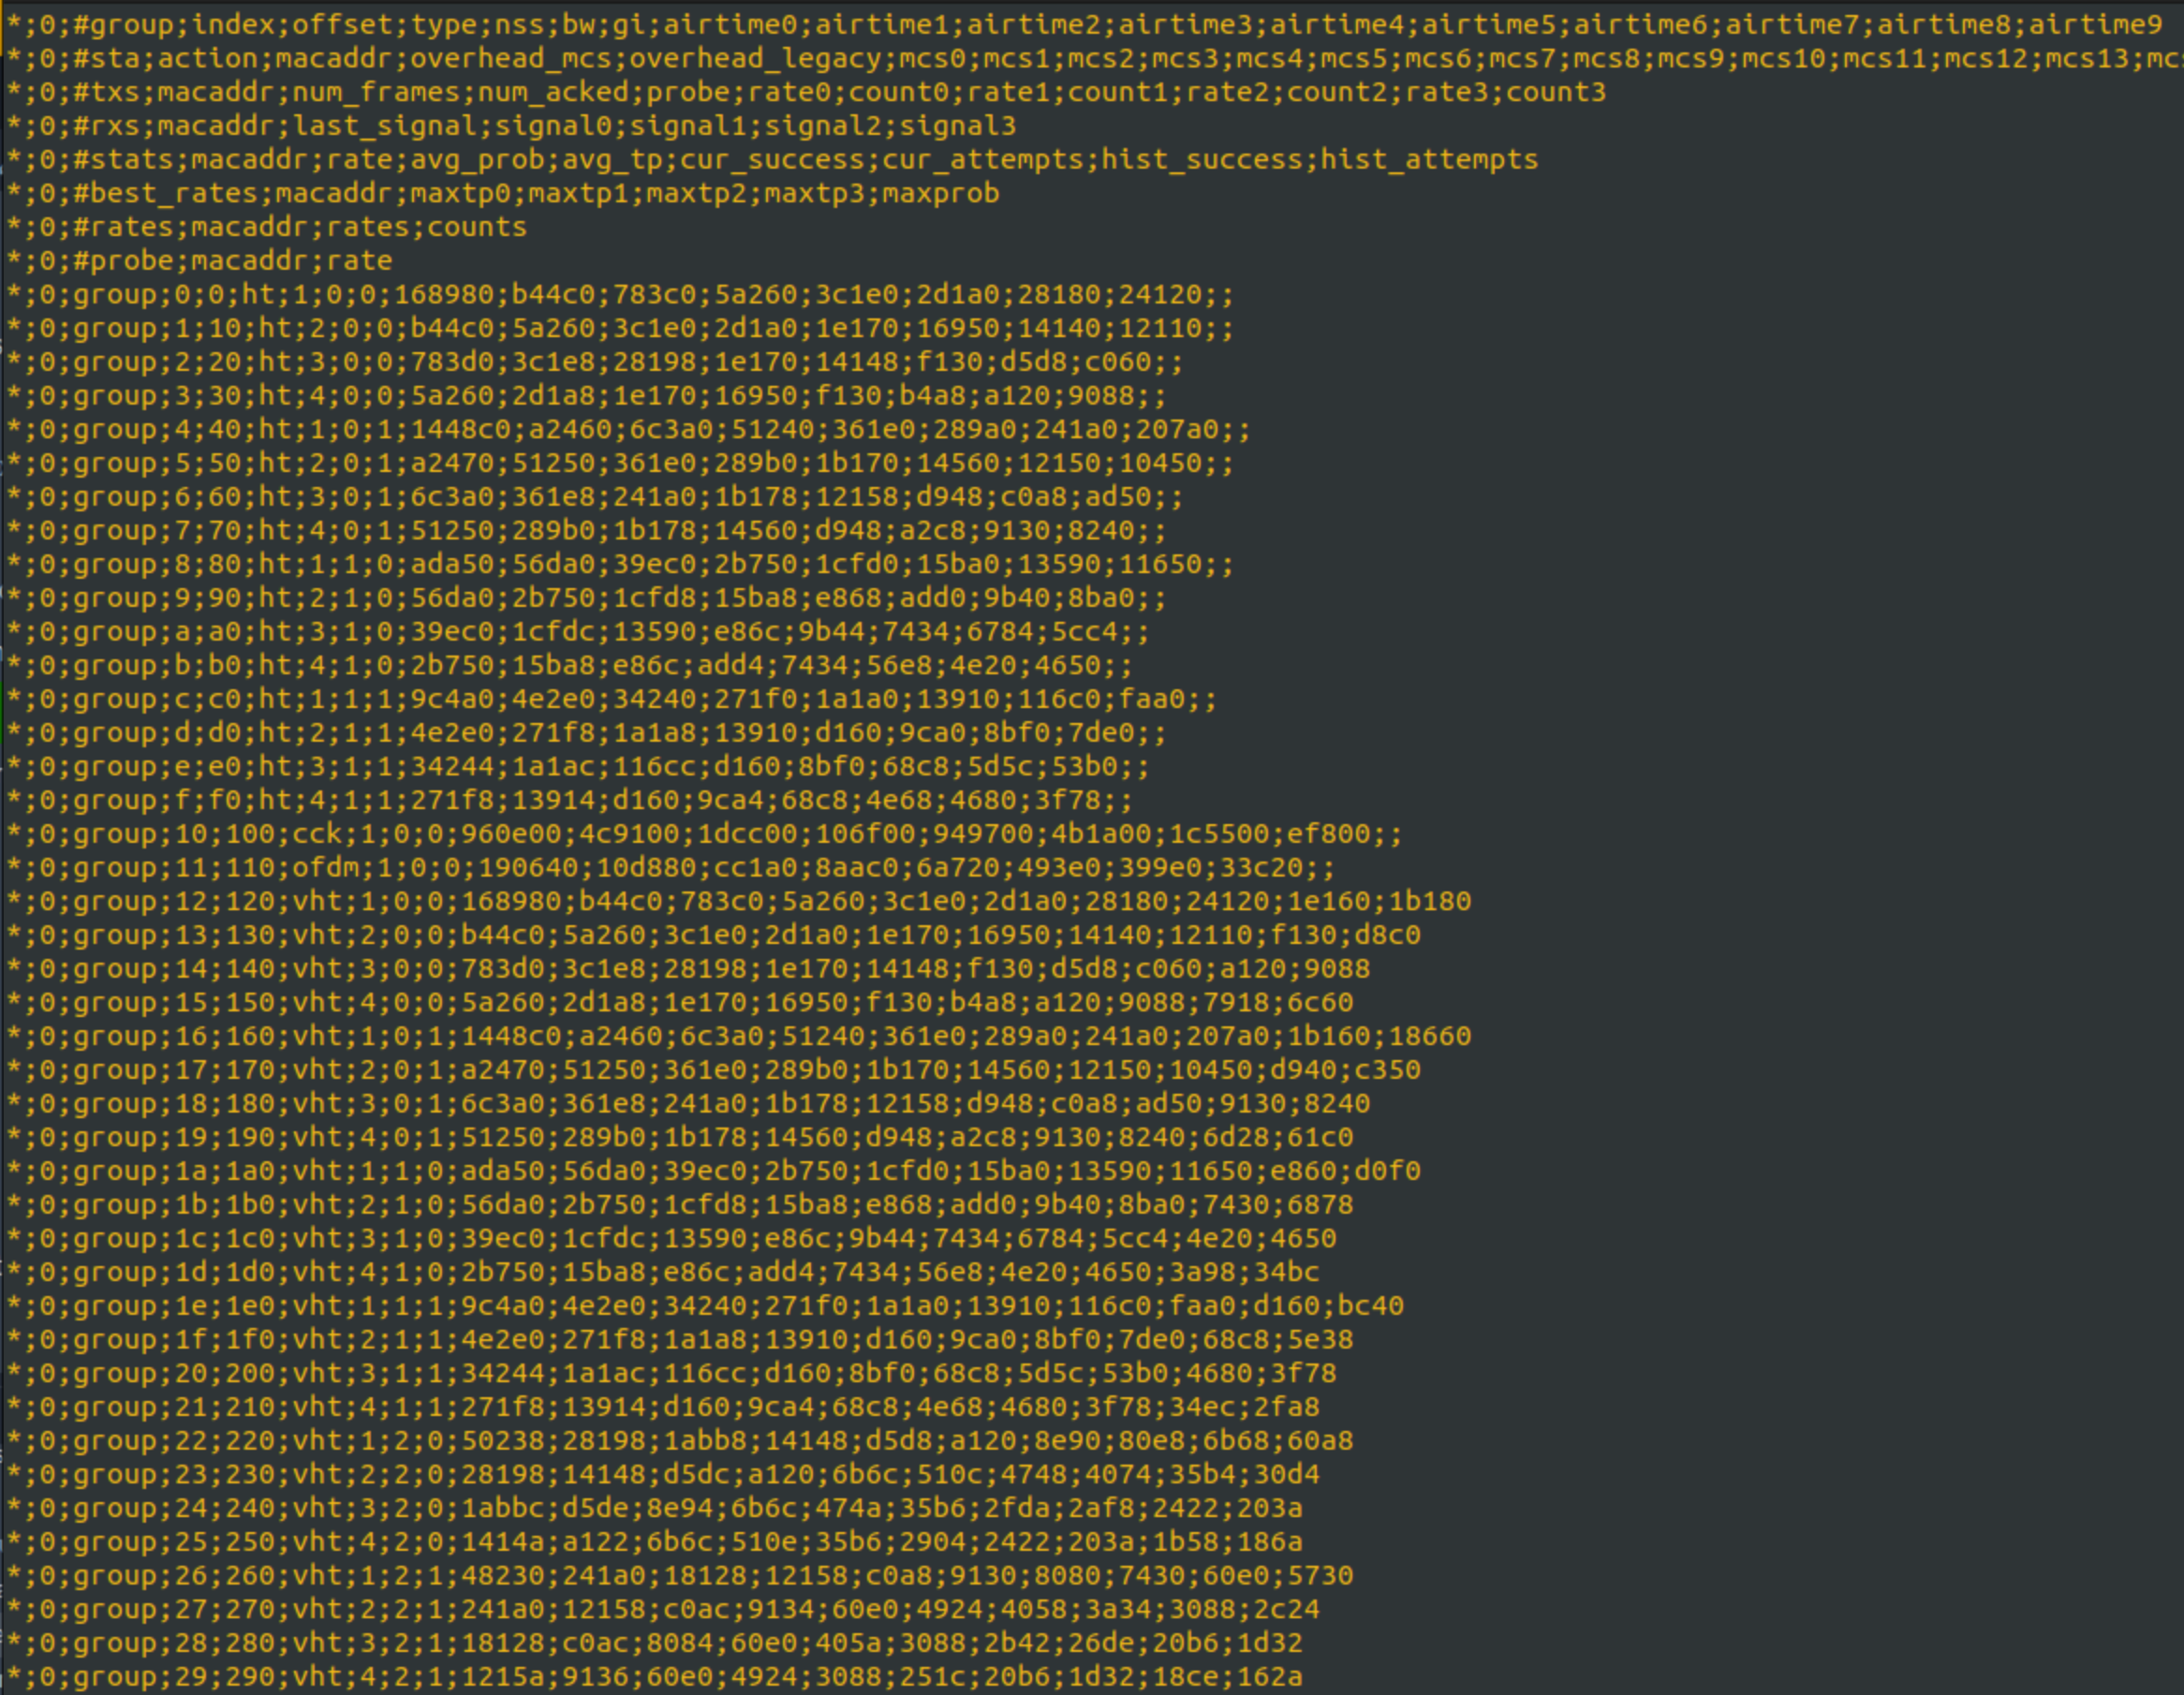
\includegraphics[width=\textwidth]{figures/plots/ratetable.png}
  \caption[Trace File Header]{Here is an example Trace file that contains the header information for GROUP, STA, TXS, RXS, STATS, and best\_rates. It proceeds to give a comprehensive breakdown of the rate specifications for 42 distinct groups.}
  \label{fig:plot_csv1}
\end{figure}

\begin{figure}[htbp]
  \centering
  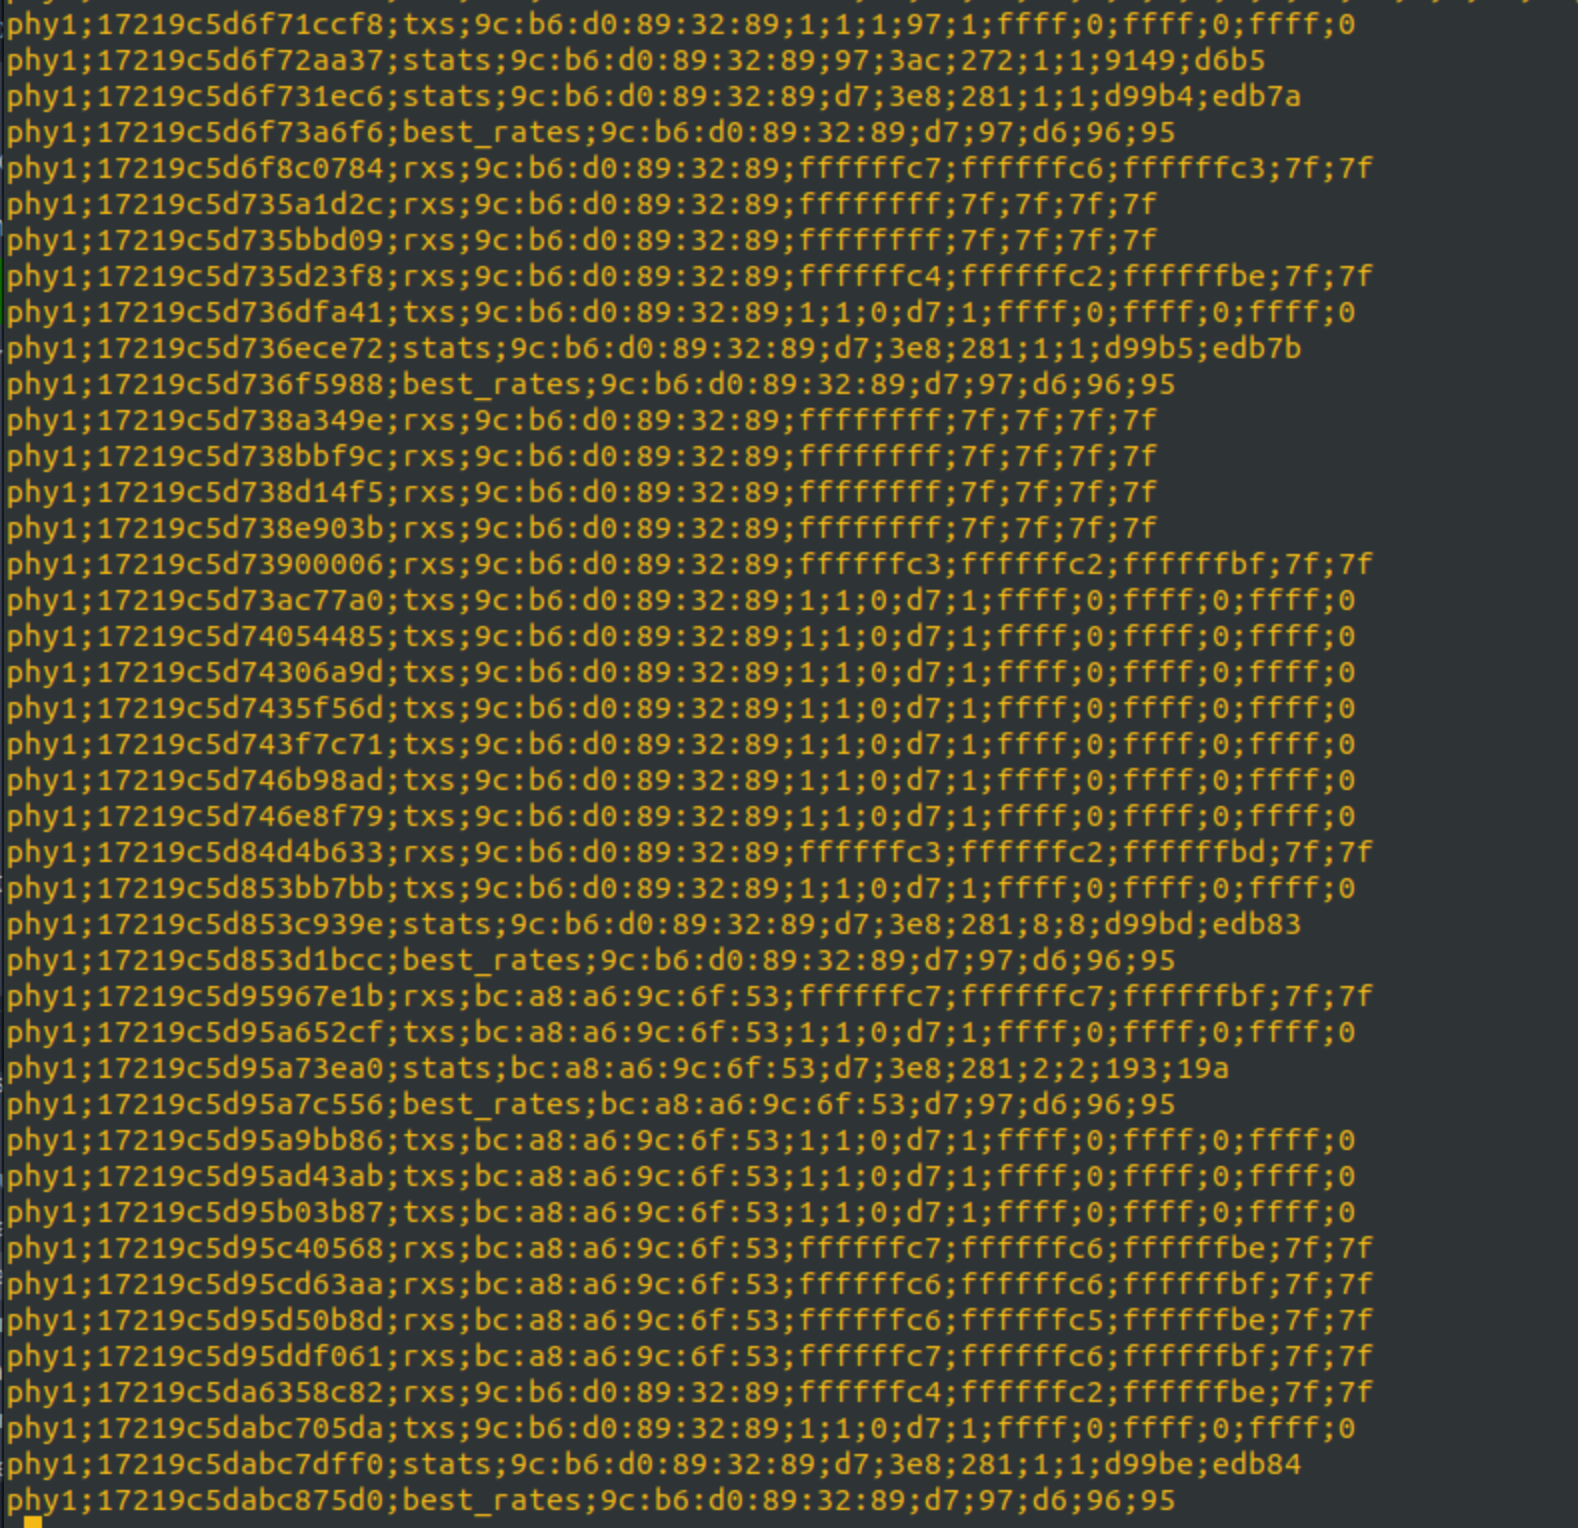
\includegraphics[width=\textwidth]{figures/plots/traceexp.png}
  \caption[Trace File Sample]{Sample of a trace file that contains informative details about transmissions, received signal strength, MAC address of connected stations to AP, and more.}
  \label{fig:plot_csv2}
\end{figure}



\begin{sloppypar}
\begin{itemize}
\item \ GROUP
\begin{lstlisting} [
basicstyle=\small
]
*;0;#group;index;offset;type;nss;bw;gi;airtime*
\end{lstlisting}
Group lines are based on The Modulation Coding Scheme(MCS)index, which has been defined by the WiFi parameters between station and wireless access point.   
    \begin{itemize}
        \item index: Specifies the hexadecimal group index (0-f), (10-1f), (21-29). Group index differs on WiFi parameters such as type, NSS, BW, GI (short guard interval).
        \item offset: Within the group, index (0-7) is being presented. The index number characterizes rates based on airtime values.
        \item type: Very High Throughput (VHT), 802.11ac standard. High Throughput (HT), 802.11n standard. Complementary code keying (CCK) is a modulation that is used by 802.11b (Only used in group 10 - Management frames being transmitted via this modulation). Orthogonal Frequency Division Multiplexing (OFDM) is adopted into 802.11a, 802.11n, 802.11ac standards (group 11 uses this modulation).
        \item nss: Number of antennas used for transmitting (TX)/receiving (RX) been aggregated in NSS (Number of Spatial Stream), which defines how many NSS can be handled by the station.
        \item bw: Bandwidth is represented as 0=20MHz, 1=40MHz, 2=60MHz, 3=180MHz.
        \item gi: Represents short guard interval in Boolean. 0=0.8µs GI, 1=0.4µs GI.
        \item airtime: Corresponds to the offset number of the rate within the group. E.g., rate~21 belongs to group~2, offset~1, airtime~1. Airtime is in nanosecond unit and has been discussed in ~\ref{sec:intro:wifiratecontrol:Group creation}.
    \end{itemize}

\item \ STA
\begin{lstlisting} [basicstyle=\small]
phy*;timestamp;#sta;action;macaddr;overhead_mcs;overhead_legacy;mcs*
\end{lstlisting}
WiFi card standards defines which rate groups are available on stations. STA lines reports this information. Based on "MCS Index,"42 group of MCS rate groups can possibly be available.

    \begin{itemize} 
        \item phy*: Defines the radio interface followed by an index.
        \item timestamp: Timestamp in UNIX nanoseconds.
        \item action: Descriptive information about the action flags presented in~\ref{sta}.
        \item macaddr: MAC address of connected stations.
        \item mcs*: 42~MCS indexes are introduced in the "sta" line. Indexes noted by "ff" indicate the availability of that rate group on the connected station.
        \begin{lstlisting}[basicstyle=\small]
        E.g., phy1;17254b11152721e0;sta;add;bc:a8:a6:9c:6f:53;6c;3c;
        ff;ff;0;0;0;0;0;0;ff;ff;0;0;ff;ff;0;0;0;0;0;0;0;0;
        0;0;0;0;0;0;0;0;0;0;0;0;0;0;0;0;0;0;0;0
        \end{lstlisting}
        A station with the MAC address "bc:a8:a6:9c:6f:53" has been added to the AP list. The groups "0, 1, 8, 9, c, d" contain the available rates on the station. 
    \end{itemize}
    
\item \ TXS
\label{txs}
\begin{lstlisting}[basicstyle=\small]
phy*;timestamp;#txs;macaddr;num_frames;num_acked;probe;rate0;count0..rate3;count3
\end{lstlisting}
Transmission of data frame been reported via TXS lines.

    \begin{itemize}
        \item num\_frames: The number of aggregated data\_frame been transmitted which represented in base16~(hex). It is possible for multiple frame transmissions to be reported in a single line of "txs" within the same timestamp.
        \item num\_acked: The number of sub-frames that have been acknowledged out of aggregated data frames is reported in base16 (hex).
        \item probe: The probe transmission rates are chosen based on the sampling interval of Minstrel HT, which is set at every 20 milliseconds in the current setup. The Boolean flag of the probe defines whether probe transmission rates are enabled or not.
        \item rate *: The chosen rates are presented with "rates*". If the value is "ffff",it shows that no other rate been tried for transmission.
        \item count *: The number of retries for each rate is reported in base16(hex). The maximum retry count per Multi-Rate Retry(MRR)stage is based on standard's protocol as shown in Table~\ref{tab:3a}. The retry attempts continues until possible count, which determines the success or failure of a transmission (It may involves all aggregated sub\_frames or only a part of them).  
        
    \end{itemize}
\begin{table}[ht]
    \centering
    \begin{tabular}{||c c c c||} 
         \hline
         Driver & IEEE 802.11 & mrr stages in hardware & retry count per mrr stage \\ [0.5ex] 
         \hline\hline
         ath5k & b/g/a & 4 & possible to configure/stage \\ 
         \hline
         ath9k & b/g/a/n & 4 & possible to configure/stage \\
         \hline
         mt76 & a/n/ac & 4 & count[0]=1 , count[1,2,3]= fixed up to 15 retries \\
         \hline
         mt76 & b/g/n & 8 & 4 per rate \\
         \hline
         mt76 & b/g/a/n/ac & 8 & 4 per rate \\ [1ex] 
         \hline
    \end{tabular}
    \caption[WiFi Chip Capabilities]{The WiFi Chip Capability table provides information on the number of retry stages and the maximum retry counts for each stage ($count{0}$,$count_{1}$,$count_{2}$,..)  for each driver.}\label{tab:3a}  
  \end{table}  
  
\item \ RXS
\label{rxs}
\begin{lstlisting}[basicstyle=\small]
phy*;timestamp;#rxs;macaddr;last_signal;signal0;signal1;signal2;signal3
\end{lstlisting}
RXS lines are Received Signal Strength values that presents measurement of the power in a received radio signal.

 \begin{itemize}
     \item last-signal: Indicated the power of last radio signal received in specified timestamp.
     \item signal[0..3]: RSSI up to four available antennas. In the rxs function of Minstrel HT algorithm signal is an 32-bit signed integer value represented in hexadecimal notation. To convert it to a decimal value, we first need to extend the sign bit, which is the most significant bit, to fill the remaining bits of the 32-bit value. In this case, the sign bit is 1, which indicates that the value is negative. The value 0x7f is a default signal strength value that is used when an antenna chain is not used to receive a frame. It is a 7-bit signed integer value that corresponds to a signal strength of -1~dBm, which is a relatively weak signal. 
     
 \end{itemize}

\item \ STATS
\begin{lstlisting}[basicstyle=\small]
phy*;timestamp;#stats;macaddr;rate;avg_prob;avg_tp;cur_success;cur_attempts;
hist_success;hist_attempts
\end{lstlisting}
The STATS includes statistics about the performance of a wireless network using the Minstrel HT algorithm.
 \begin{itemize}
     \item rate: This field indicates the transmission rate that is being used by the client device. For each rate been used there is a stats lines presented. 
     \item avg-probe: The average probability of success for transmissions at that rate.
     \item avg-tp: The average throughput achieved by the client device at that rate.
     \item cur-success: The number of successful transmissions at the current rate.
     \item cur-attempts: The number of attempted transmissions at the current rate
     \item hist-success: This field represent the number of successful for the current rate and all previous rates used by the client.
     \item hist-attempts: Defines the number of attempted transmissions for the current rate and all previous rates used by the client.
 \end{itemize}
This information can be used to evaluate the performance of a wireless network and to adjust the transmission rates used by individual station in order to optimize performance.

\item \ BEST\_RATES
\label{bestrates}
\begin{lstlisting}[basicstyle=\small]
phy*;timestamp;#best_rates;macaddr;maxtp0;maxtp1;maxtp2;maxtp3;maxprob
\end{lstlisting}
The "best-rates" lines refer to the best transmission rates for each of the streams available in the wireless device. The $maxtp_{0}$, $maxtp_{1}$, etc. variables represent the maximum throughput achieved for each of the best transmission rates for the respective streams. The $max_{prob}$ value in the output of the algorithm indicates the highest estimated probability of success among all the available rates for a particular client device.

\end{itemize}
\end{sloppypar}

\subsection{Capabilities}
\label{sta}
In Minstrel HT algorithm, to determine the optimal transmission rate for each station based on the current wireless channel conditions, the algorithm maintains a set of data structures that track the past transmissions and their outcomes for each station.
the following commands are used to manage station information via STA lines.
\begin{itemize}
\item \ sta;add  
To add a new station to the algorithm, the "ADD" function is used. When a new station joins the network, the algorithm initializes its data structures with default values and starts collecting data on its transmissions.
\item \ sta;update
After each transmission, the "UPDATE" function updates the data structures for a given STA. The algorithm keeps track of the success or failure of each transmission and updates the relevant data structures accordingly. The updated data is then used to determine the optimal transmission rate for the station for the next transmission.
\item \ sta;remove 
When a station leaves the network, the "REMOVE" function is used to remove its data structures from the algorithm, and its transmissions are no longer considered in the rate control decisions.
\end{itemize}
\newpage





\section{Summary}

The chapter describes the data collection setup and the format of the monitoring information used in the analysis. The experiment involved an Atheros~AR9287 wireless chip, and the stations connected to the AP were diverse and located in various positions and orientations~\ref{sec:Measurement Tools:Data collection Setup}. Then focuses on data trace files fetched from the Linux kernel, and unfurls descriptive details about the headers and all related details present on trace files, such as the definition of each header value, the unit of them and much more~\ref{sec:Measurement Tools:Format of Monitoring Information}.
\chapter{Analysis and Optimization}
\label{chap:Analysis and Optimization}

The objective of this chapter is to introduce~\ref{sec:Analysis and Optimization:Implementation of an Analysis Tool} and evaluate the performance of the Minstrel-HT rate control algorithm in wireless networks~\ref{sec:Analysis and Optimization:Performance Evaluation}. To accomplish this, a Python-based tool was developed to extract data from the Linux kernel trace file and generate various analytical plots for quantitative analysis of the data transmission process. The tool provides a detailed observation of multiple aspects, including the number of transmitted frames, the number of ACK and Non-Ack frames and their probability and additional metrics.

By utilizing the Python-based tool, we generated a diverse set of analytical plots to observe and analyze the network. In sub-chapter \ref{sec:Analysis and Optimization:Implementation of an Analysis Tool}, we will provide a detailed description of each analytical plot, including the calculation methodology employed to derive the values presented in each plot. We will also explain the significance of these observations, the chosen presentation format for the plots, and showcase the key insights derived from them. In the next step, sub-chapter~\ref{sec:Analysis and Optimization:Performance Evaluation}, performance cases of the Minstrel-HT algorithm will be discussed in a real scenario desk setup environment that was accessible and introduced in~\ref{chap:Measurement Tools}\ref{sec:data_set}.

Through the analysis of these plots, a deeper understanding of the data transmission environment and network parameters can be obtained, enabling the path through evaluation of the Minstrel-HT algorithm and will aid in optimizing and analysing new algorithms and enhancing the overall effectiveness of wireless networks.
\newpage

\section{Implementation of an Analysis Tool}
\label{sec:Analysis and Optimization:Implementation of an Analysis Tool}
The trace files taken from Linux Kernel performed by the Minstrel-HT algorithm contains lots of information about it's performance in real-world scenarios, as previously detailed in section~\ref{sec:Measurement Tools:Format of Monitoring Information}. In this section, a quantitative evaluation and calculations of the data-set (Figure \ref{fig:plot_csv2}) will be provided to offer comprehensive insights into the observations made. 
In the plots presented in Section~\ref{sec:Analysis and Optimization:Performance Evaluation}, a range of parameters has been utilized. In this section, we describe the calculation methodology for each parameter. Each line of the data-set will be evaluated and compared to the corresponding analytical plot. This analytical approach facilitates the generation of observations that contribute to a deeper understanding of the algorithm's behavior. Furthermore, it provides a representation of the channel environment and network parameters, along with additional insights into the quality of the wireless channel through the power level of the received signal.

\newpage
\subsection{Available rates}
\label{sec:Analysis and Optimization:Implementation of an Analysis Tool:AvailableRates}

The STA line(as introduced in detail~\ref{sec:Measurement Tools:Format of Monitoring Information} )in the trace files~\ref{fig:plot_csv2} presents crucial information regarding the available rates for each station connected to the AP. By carefully examining this data, we can discover why certain rates are used more frequently than others, or why some rates may not be used at all. Indeed, the number of available rates are fully dependent on connected station and rate availability based on the WiFi chip. Older or lower-end devices may not support the higher MCS rates available in newer Wi-Fi protocols. For example, an older Station with a Wi-Fi chip that only supports the 802.11n protocol may not be able to handle the higher MCS rates available in the newer 802.11ac protocol. In such cases, the access point may automatically adjust the MCS rate to match the capabilities of the client device. The availability of rates are observable via this type of plot.fig~\ref{fig:STA}

As described in the~\ref{sec:intro:wifiratecontrol:Group creation}, in the scope of this thesis, when we talk about a group, we are referring to the aforementioned method which is used by Minstrel-HT. As shown in the plot, the y-axis focuses on groups, and the x-axis produces the indexes within each group. The y-labels are (Type-Numbers of spatial stream-Guard interval and Bandwidth), and the x-axis focuses on the available MCS within each group. The available rates for our station to use for data transmission are shown in white, while all other group rates in black are unavailable for transmission. In the scope of this thesis, Type VHT is unavailable for the ath9k WiFi-chip. All not available rates in future plots will have an "NA" label to reduce confusion and simplify the look.

This plot~\ref{fig:STA} was generated by analyzing STA lines, as shown in the example below, the device with the MAC address bc:a8:a6:9c:6f:53 added to the trace lines. After the MAC address value, 42 spaces are displayed, corresponding to rate groups. "FF" indicates that the rate group is available for data transmission, while "0" indicates that the rate group is unavailable.
Analysing STA lines can provide valuable information about the availability of rates in the network chip-set of connected devices. By monitoring the availability of rate groups, researcher can make informed decisions about network optimization and troubleshooting.

\begin{lstlisting} [basicstyle=\small]
phy1;17254b11152721e0;sta;add;bc:a8:a6:9c:6f:53;6c;3c;
        ff;ff;0;0;0;0;0;0;ff;ff;0;0;ff;ff;0;0;0;0;0;0;0;0;
        0;0;0;0;0;0;0;0;0;0;0;0;0;0;0;0;0;0;0;0
\end{lstlisting}
\newpage
\subsection{MAC-Based Transmission and Station Population: A Time-Series Analysis}
\label{population}
In real-life scenarios, multiple stations are often connected to an access point (AP). To better observe channel activity, plot~\ref{fig:plot_22_population} has been created to analyze the availability of each station in the channel. 
The y-axis displays the MAC address of each connected station, while the x-axis provides a time label. Depending on the radio being leveraged for transmission, either PHY~0 or PHY~1 can be observed in the plot.

It is important to note that analyzing channel activity can provide valuable insights into network performance and can help identify potential issues such as interference or congestion. The plots were generated by analysing "txs" lines, which utilize timestamps (UNIX nanosecond) as a time indicator and MAC addresses as available stations. This allows for the identification of the specific time at which transmission occurred for each station, regardless of the success or failure of the packet transmission.
\vspace{0.5cm}
\begin{lstlisting}[basicstyle=\small]
phy*;timestamp;#txs;macaddr;num_frames;num_acked;probe;rate0;count0..
\end{lstlisting}


\subsection{Temporal Analysis of signal strength value}
\label{RSSI}
The plots were generated to increase our awareness of signal strength values over time. Based on \ref{rxs}line in trace file, "Last-signal" indicates the power of the last radio signal received at a specified timestamp. 
The x-axis represents time (day:hour:minute:second), while the y-axis displays the last signal value. The signal is a 32-bit signed integer value represented in hexadecimal notation.The plot is also grouped based on each connected station.

In ATH9K wireless driver for Atheros-based~802.11n and 802.11ac wireless LAN devices, the following signal strength levels are commonly used to indicate signal quality:
\begin{itemize}
    \item Excellent/strong signal: above -60 dBm
    \item Good/moderate signal: between -60 dBm and -70 dBm
    \item Fair/weak signal: between -70 dBm and -80 dBm
    \item Poor/very weak signal: below -80 dBm
\end{itemize}
It is important to note that these values may vary depending on the specific device, environment, and other environmental factors.
\vspace{0.5cm}

\begin{lstlisting}[basicstyle=\small]
phy*;timestamp;#rxs;macaddr;last_signal;signal0;signal1;signal2;signal3
phy1;1723722be1f89a14;rxs;32:3b:67:22:c4:16;ffffffbe;ffffffbb;ffffffb5;7f;7f
\end{lstlisting}



\subsection{Transmission Status }
\label{sec:Analysis and Optimization:Implementation of an Analysis Tool:attempt-count}

The transmission status plot (see Fig~\ref{fig:Attempt1}) has been generated from the TXS lines~\ref{txs}. The rates which are used for packet transmission are displayed in this plot. The x-axis represents the Modulation and Coding Scheme (MCS) within each group, while the y-axis shows all available groups. The group labels are shown in detail to specify each group's Type, Numbers of spatial stream, Guard interval, and Bandwidth. "NA" values refer to Not available rates. Unavailability is directly related to limitations of the WiFi chip-set used in the connected station. More detail about available rates are described fully in~\ref{sta}, \ref{sec:Analysis and Optimization:Implementation of an Analysis Tool:AvailableRates}. The plot~\ref{fig:Attempt1} features a color bar with a logarithmic scale that displays the number of transmitted packets for each rate. The time scale is indicated in the plot's description, which allows for observation of transmitted packets for each rate on a different time scale. To achieve the value of packet transmission (ACK and non-ACK packets) per data rate following calculations are needed, notice that the value num\_frames are in hexadecimal format. Calculation of full transmission (ACK and non-ACK packets):
\vspace{0.25cm}

For $rate_0$: $count_0 \times \text{num\_frame}$ 

For $rate_1$: $count_1 \times \text{num\_frame}$ 

For $rate_2$: $count_2 \times \text{num\_frame}$ 
\vspace{0.25cm}

As for the mathematical equation:

Full Transmission for $rate_i$: $count_i \times \text{num\_frame}$

\vspace{0.25cm}
\begin{lstlisting}[basicstyle=\small]
phy*;timestamp;#txs;macaddr;num_frames;num_acked;probe;rate0;count0..
phy1;17259302480d7d3f;txs;72:63:85:2b:6c:cf;13;11;0;c7;2;c2;1;ffff;0;ffff;0
\end{lstlisting}
In the previously written TXS line, the transmission calculation can be expressed mathematically as follows:\\
Transmission for Rate Group C and MCS 2 = count * num\_ack \\
Transmission for Rate Group C and MCS 7 = count * num\_ack \\

where "count" is a numerical value representing the count for the given rate group and modulation and coding scheme, and "num\_ack" is the number of acknowledgment packets transmitted, expressed in hexadecimal format. To convert the hexadecimal value of "num\_ack" to decimal format, it can be expressed as 13\_hex, which is equivalent to 19\_decimal:\\

Transmission for Rate Group $C_7$: $2 \times 19 = 38$

Transmission for Rate Group $C_2$: $1 \times 19 = 19$
\newpage

\subsection{Acknowledged transmissions}
Acknowledgment frames indicate successful transmissions, and can be retrieved from the "txs"~\ref{txs} lines. To extract the maximum amount of information from these successful transmissions, different types of plots are created for analysis. These plots enable detailed examination of the transmission rates, modulation and coding schemes, and other relevant parameters. Further details on these plots and their applications will be described in Subsection~\ref{sec:Analysis and Optimization:Implementation of an Analysis Tool:success-count}, Subsection~\ref{Probability of Success for Rate-Based Transmission}, Subsection~\ref{sec:Analysis and Optimization:Implementation of an Analysis Tool:airtime-succespb}, and Subsection~\ref{rolling-success}.

\subsubsection{Rate-Based Packet Success Analysis}
\label{sec:Analysis and Optimization:Implementation of an Analysis Tool:success-count}
The plot (see Fig~\ref{fig:Success-count1}) is generated based on the number of frames successfully transmitted per rate. The axis of the plot have been described earlier in this section. When a specific $rate_i$ is used for transmission and there is no other following $rate_i+1$ being used, we consider that $rate_i$ to be successfully transmitted. To calculate the number of successful frames for a particular rate, we use the following formula:

\vspace{0.25cm}
1 * num\_acked
\vspace{0.25cm}

Here, num\_acked represents the number of frames acknowledged by the receiver, which is given in hexadecimal format. To perform the calculation, hexadecimal value of num\_acked is converted to its decimal equivalent.

Example:

\begin{lstlisting}[basicstyle=\small]
phy*;timestamp;#txs;macaddr;num_frames;num_acked;probe;rate0;count0..
phy1;1725ed10e65ec5f6;txs;b0:f1:d8:50:92:c1;13;11;1;c7;1;d2;2;ffff;0;ffff;0
\end{lstlisting}


The calculation based on given "txs" line for Rate-Based Packet Success:

$d_2$: $1 \times 11_{(hex)} = 1 \times 17_{(decimal)} = 17$


\subsubsection{Probability of Success for Rate-Based Transmission}
\label{Probability of Success for Rate-Based Transmission}
The plot~\ref{fig:Success-probability1} displays the probability of each transmission rate being successfully transmitted. This probability is calculated based on the transmission value for each rate. If rate $c_2$ is transmitted 30 times and only 10 transmissions are acknowledged, the successful probability for rate $c_2$ is $1/3$. The color bar the plot displays the probability (ranging from 0 to 1) for each rate.

\subsubsection{Airtime-Based Success Probability for Rate-Based Transmission}
\label{sec:Analysis and Optimization:Implementation of an Analysis Tool:airtime-succespb}

In Sections~\ref{sec:intro:wifiratecontrol:Group creation} and~\ref{txs}, the concept of "airtime" has been thoroughly described. It is crucial to understand the successful transmission probability associated with different airtime values under various real-time scenarios. To simplify this understanding, we present a plot in Figure~\ref{fig:Success-p-vs-airtime1}. It displays the values of airtime on the x-axis and the probability of successful packet transmission, which is calculated based on the rates in~\ref{Probability of Success for Rate-Based Transmission}, on the y-axis. The key difference between this plot and~\ref{Probability of Success for Rate-Based Transmission} is that the rates are translated into their corresponding airtime values~\ref{tab:airtime-success}. Each rate in the table has a corresponding airtime value, and this plot allows us to visualize how changes in airtime value can affect the probability of successful packet transmission. This information is valuable for optimizing transmission parameters in real-world scenarios, where airtime utilization and transmission reliability are critical factors to consider.
\newpage
\begin{table}[ht]
    \centering
    \begin{tabular}{|c|c|}
        \hline
        \textbf{Rate} & \textbf{Airtime Value} \\
        \hline
        0 & 168980 \\
        1 & b44c0 \\
        2 & 783c0 \\
        3 & 5a260 \\
        4 & 3c1e0 \\
        5 & 2d1a0 \\
        6 & 28180 \\
        7 & 24120 \\
        10 & b44c0 \\
        11 & 5a260 \\
        12 & 3c1e0 \\
        13 & 2d1a0 \\
        14 & 1e170 \\
        15 & 16950 \\
        16 & 14140 \\
        17 & 12110 \\
        80 & ada50 \\
        81 & 56da0 \\
        82 & 39ec0 \\
        83 & 2b750 \\
        84 & 1cfd0 \\
        85 & 15ba0 \\
        86 & 13590 \\
        87 & 11650 \\
        90 & 56da0 \\
        91 & 2b750 \\
        92 & 1cfd8 \\
        93 & 15ba8 \\
        94 & e868 \\
        95 & add0 \\
        96 & 9b40 \\
        97 & 8ba0 \\
        \hline
    \end{tabular}
    \caption[Airtime Value For Transmission Rates]{The table displays the airtime values in the table are transmission time in unit nanoseconds, shown in hex value.  Each rate has its airtime value calculated in the Minstrel-HT algorithm. The tables contain the airtime of rates within Groups 0, 1, 8 and 9. The full version of airtime table in present in~\ref{fig:plot_csv1}}
    \label{tab:airtime-success}
\end{table}

\newpage

\subsubsection{Probability of Success for Rate-Based Transmission with Rolling Time Averages}
\label{rolling-success}
Rolling time window is a statistical technique used in time-series analysis, which involves applying a function to a sliding window of data points in a time series. The function is applied over a specified window or time interval and is then moved to the next window, allowing for a rolling calculation over time. The rolling time window technique has many applications in time series analysis, such as smoothing noisy time series data, identifying trends and patterns, and detecting anomalies or outliers. By using rolling time windows, we can smooth out short-term fluctuations in the data-set and focus on the longer-term observations. Rolling time windows can also help us to identify changes in the statistical properties of a time series over time, such as changes in the mean or variance. This is particularly useful when dealing with non-stationary time series data, which may exhibit changes in statistical properties over time. By using rolling time windows, we can detect and analyze these changes in a more robust and accurate way~\cite{pandas_rolling}.

In the context of this thesis, data frames are being transmitted in the temporal base. While we have already plotted the probability of success (see Fig~\ref{fig:Success-probability1}), such an aggregate value is insufficient to observe changes in over time scenarios. To address this, we have adopted the rolling value technique which provides a smooth and timely view of the changes. This approach allows us to observe the channel at any given time and obtain insights into the ongoing transmissions. Notably, the rolling time value can be modified, and for this thesis, it has been set at 100~ms to match the MRR chain that is also being updated every 100~ms. By using this technique, we can obtain a detailed understanding of the temporal behavior of the transmissions and the channel.

On the x-axis of the plot(see Fig~\ref{fig:Rolling-Success1}), the time parameter is represented, while the y-axis displays all the available rates for the ath9k~chip, specifically the high-throughput rate type. The color bar ranging from 0 to 1 denotes the probability of a successful transmission. It is worth noting that each scatter dot in the plot represents the calculated success probability in rolling time windows of 100ms.
\newpage
\subsection{Non-acknowledged transmissions}

Understanding and analyzing failed transmissions can provide valuable insights into the performance of a wireless network. By identifying the causes of failures, we can take steps to improve the quality and reliability of the network. In general cases some common causes of failed transmissions include interference from other wireless devices, signal attenuation due to distance or obstacles, and incorrect configurations of the wireless access points.

In order to better understand the nature of failed transmissions, it is important to check the "txs" report. As been descriptively focused on this topic~\ref{txs} The report provides detailed information about each transmission, including the physical address of the sender/receiver, the number of data frames transmitted, and the acknowledgement status of each frame. By analyzing this information, it is possible to identify patterns in the occurrence of failed transmissions, such as specific devices or locations that are more prone to interference or signal degradation. An example of a "txs" report is shown below:
\vspace{0.2cm}

phy1;1725ed10e531013a;txs;b0:f1:d8:50:92:c1;1;1;1;d3;1;d2;1;ffff;0;ffff;0
\vspace{0.2cm}

The report implies that a transmission was attempted from the device with the physical address "b0:f1:d8:50:92:c1" using the $phy{1}$ wireless interface. Number of data frames is one, and it is acknowledged. Rate $d{3}$ was attempted once but failed, while $d{2}$ was used and resulted in a successful transmission.

\subsubsection{Rate-Based Packet Failure Analysis}
\label{failed-count}
The Figure~\ref{fig:Fail-count1} represents the number of frames that have not been successfully transmitted, categorized by transmission rate. The axis of this graph have been previously unwrapped. The computation of failed packet transmissions proceeds as follows:

As mentioned earlier in sections~\ref{sec:Analysis and Optimization:Implementation of an Analysis Tool:attempt-count} and~\ref{sec:Analysis and Optimization:Implementation of an Analysis Tool:success-count}, the values for transmitted packets and successfully transmitted packets are instantly available. By subtracting these two values, we can determine the number of failed or Non-Acknowledged packets for each transmission rate.
\begin{lstlisting}[basicstyle=\small]
phy*;timestamp;#txs;macaddr;num_frames;num_acked;probe;rate0;count0..
phy1;1725ed10e531013a;txs;b0:f1:d8:50:92:c1;1;1;1;d3;1;d2;1;ffff;0;ffff;0
\end{lstlisting}

Transmitted packets per rate: $d_3$= 1, $d_2$=1

Acknowledged (successful) transmissions: $d_2$=1

\vspace{0.25cm}

Non-acknowledged (failed) transmissions:

[Transmitted packets per rate] - [Acknowledged (successful) transmissions] = rate $d_3$ with 1 failed packet
\newpage
Another example: 
\begin{lstlisting}[basicstyle=\small]
phy*;timestamp;#txs;macaddr;num_frames;num_acked;probe;rate0;count0..
phy1;1725ed10e65ec5f6;txs;b0:f1:d8:50:92:c1;13;11;1;c7;1;d2;2;ffff;0;ffff;0
\end{lstlisting}
First, the hexadecimal values of `num\_frames` and `num\_acked` will be converted to decimal. Subsequently, the calculation will be carried out as previously described.

num\_frames: 13 (hex) = 19 (decimal)

num\_acked: 11 (hex) = 17 (decimal)

Transmitted packets per rate:

$c_7=1\times19=19$

$d_2=2\times19=38$

Acknowledged (successful) transmissions:

$d_2=1\times17=17$

Non-acknowledged (failed) transmissions:

For rate $c_7$:

[Transmitted rates $c_7$] - [Acknowledged (successful) transmissions $c_7$] = 19 - 0 = (19 failed packets)

For rate $d_2$: 

[Transmitted rates $d_2$] - [Acknowledged (successful) transmissions $d_2$] = 38 - 17 = (21 failed packets)

\subsubsection{Probability of Failure for Rate-Based Transmission}
\label{failedprobability}
The plot presented in Figure~\ref{fig:Fail-probability1} represents the probability of failure for each transmission rate. This value is computed by dividing the number of failed packets, as recorded by the function~\ref{failed-count}, by the number of attempted packets, as recorded by the function ~\ref{sec:Analysis and Optimization:Implementation of an Analysis Tool:attempt-count}.

To clarify, the failed probability refers to the likelihood that a packet sent at a given rate will not be successfully transmitted. The results presented in Figure~\ref{fig:Fail-probability1} provide insights into the performance of rate-based transmission systems, as they indicate which rates are most susceptible to failure in given scenarios.

\subsubsection{Rate-Based Transmission Failure Analysis with Rolling Time Averages}
\label{Rolling-fail}
As discussed in Section~\ref{rolling-success}, the rolling value is a critical metric for analyzing rate-based transmission systems. By extracting 100ms of data from our trace file, we can calculate the probability of failure for each rate. This value is continuously updated by rolling over the data and recalculating the probabilities every 100ms.

As shown in Fig~\ref{fig:Rolling-Fail1}, x-axis represents the rolling time, and y-axis displays the rate group (number, modulation and coding scheme, bandwidth, bandwidth status, and number of special streams.) Each label provides a descriptive version of the group rate index, allowing us to better monitor the performance of each rate over time. This plot allows us to focus on specific rate parameters, such as the guard interval, and the probability of failure is color-coded on a scale of 0 to 1. 
% We can also group the rates by bandwidth, guard interval, or special stream only\ref{sec:extra_plots}.

These types of plots, such as Figures~\ref{fig:Rolling-Fail1} and~\ref{fig:Rolling-Success1}, are valuable tools for analysing rate-based transmission systems and identifying areas for improvement. By monitoring the probability of failure over time and focusing on specific rate parameters, we can optimize the performance of our system and reduce the risk of failure.


\subsection{Overlap of Packet Success \& Failure with Rolling Time Average }
\label{Overlap}

As part of the optimization process, it was interesting to investigate and observe the overlap between Non-ACK and ACK rates. To calculate the overlap values, a rolling function was utilized with a time window of 100~ms, as shown in Fig~\ref{fig:overlap1}. To provide a numerical example of how the overlap value is calculated:

\begin{lstlisting}[basicstyle=\small]
phy1,2022-10-26 12:32:39.817,txs,b0:f1:d8:50:92:c1,1,1,1,c2,1,c1,1,ffff,0
phy1,2022-10-26 12:32:39.827,txs,b0:f1:d8:50:92:c1,1,1,0,c2,1,ffff,0,ffff,0
phy1,2022-10-26 12:32:39.834,txs,b0:f1:d8:50:92:c1,1,1,0,d1,1,ffff,0,ffff,0
phy1,2022-10-26 12:32:39.844,txs,b0:f1:d8:50:92:c1,1,1,0,d2,1,ffff,0,ffff,0
phy1,2022-10-26 12:32:39.856,txs,b0:f1:d8:50:92:c1,1,1,1,95,1,94,3,ffff,0
phy1,2022-10-26 12:32:39.867,txs,b0:f1:d8:50:92:c1,29,29,0,d2,1,ffff,0
phy1,2022-10-26 12:32:39.877,txs,b0:f1:d8:50:92:c1,1,1,0,d7,1,ffff,0,ffff,0
phy1,2022-10-26 12:32:39.888,txs,b0:f1:d8:50:92:c1,1,1,0,d7,1,ffff,0,ffff,0
phy1,2022-10-26 12:32:39.890,txs,b0:f1:d8:50:92:c1,1,1,1,95,1,ffff,0,ffff,0
\end{lstlisting}
\vspace{0.5cm}

To solve an optimization problem that depends on multiple variables, it is often necessary to normalize the values of these variables. In the present case, we use the overlap value, defined as the minimum of successful and failed transmission counts divided by the sum of these counts. Mathematically, we can express this as:

\begin{equation}
Overlap\ value = \frac{min(Successful\ transmission\ count,\ failed\ transmission\ count)}{Successful\ transmission\ count + failed\ transmission\ count}
\end{equation}

This operation ensures that both successful and failed transmission counts have equal weight in the function being minimized. The overlap value can thus be used as a useful tool for optimizing performance in various applications.
\newpage
After calculating the overlap value using the provided formula, it is observed that in cases where there is an equal count of successful and failed packets, the overlap value is maximum. Conversely, when there is no intersection, the overlap value is zero. A full overlap is indicated by a value of 0.5 using the overlap value, whereas a value of zero indicates no overlap.

According to the Principle of Indifference, also known as the Principle of Insufficient Reason, if two events have equal probability, the probability of either one occurring is 0.5. This principle is a fundamental concept in probability theory and decision theory, and it is widely used in various fields of study.

The principle states that when there is a set of equally likely outcomes and there is no additional information or reason to prefer one outcome over another, then each outcome should be assigned an equal probability. This means that if there are two equally likely outcomes, the probability of either one occurring is 0.5.

The mathematical reference for this principle is based on the axioms of probability theory, which state that probabilities must satisfy certain properties such as being non-negative and adding up to 1. The Principle of Indifference is a way of assigning probabilities to events when there is no other information available, and it ensures that the probabilities assigned are consistent with the axioms of probability theory.

For instance, in the case of flipping a fair coin, since the coin is equally likely to land on heads or tails, the probability of getting heads is 0.5, and the probability of getting tails is also 0.5. In this case, there is no reason to prefer one outcome over the other, so each outcome is assigned an equal probability of 0.5.

Similarly, in Overlap\_value formula, if Successful\_transmission\_count and Failed\_transmission\_counts are equal, the minimum value between them would also be equal, resulting in a probability of 0.5. This follows the Principle of Indifference, where if there is no reason to prefer one outcome over another, each outcome should be assigned an equal probability of 0.5.
Due to this principle we must Normalize the calculated Overlap, via normalization formula:

\begin{equation}   
x_{norm} = \frac{x - x_{min}}{x_{max} - x_{min}}
\end{equation}


\begin{flalign*}
&\text{Normalized-Overlap}_{94} = \frac{0.33 - 0}{0.5 - 0} = 0.66 && \\
&\text{Normalized-Overlap}_{95} = \frac{0.5 - 0}{0.5 - 0} = 1 && \\
&\text{Normalized-Overlap}_{d_1,d_2,d_7,c_1,c_2} = \frac{0 - 0}{0.5 - 0} = 0 &&
\end{flalign*}

At the end of the process, the average value of "Normalized overlap" is calculated, providing a single value for 100ms of packet transmission. This value is presented in Figure \ref{fig:overlap1}, where the x-axis represents the rolling time window value and the y-axis represents the normalized average overlap value ranging from 0 to 1.
Consider the following scenario: we want to create a plot to represent our data. The x-axis of the plot will contain a single time stamp, which acts as an indicator for the first timestamp, and it will roll for 100~ms. On the y-axis, the plot will display the average overlap value of 0.8.
\vspace{2cm}
\begin{table}[ht]
\centering
\begin{tabular}{|c|c|c|c|cl}
\hline
Rate & \multicolumn{1}{p{2.5cm}|}{\centering Successful\ transmissions} & \multicolumn{1}{p{2.5cm}|}{\centering Failed\ transmissions} & \multicolumn{1}{p{2.5cm}|}{\centering Overlap} & \multicolumn{1}{p{2.5cm}|}{\centering Normalized\ Overlap}\\
\hline
94 & 1 & 2 & 0.33 & 0.6\\
\hline
95 & 1 & 1 & 0.5 & 1\\
\hline
d1 & 1 & 0 & 0 & 0 \\
\hline
d2 & 2 & 0 & 0 & 0 \\
\hline
d7 & 2 & 0 & 0 & 0 \\
\hline
c1 & 2 & 0 & 0 & 0 \\
\hline
c2 & 0 & 1 & 0 & 0 \\
\hline
Avg Overlap & \multicolumn{4}{c|}{0.8} \\
\hline
\end{tabular}
\caption{Overlap calculation}
\label{tab:overlap}
\end{table}


\newpage
\section{Performance Evaluation}
\label{sec:Analysis and Optimization:Performance Evaluation}

In this section, real-world scenarios are examined to demonstrate the effectiveness and applicability of the analytical tool in assessing the performance of Minstrel-HT. By presenting a series of case studies, the goal is to clarify the practical outcomes of the findings and provide insights that can be obtained from the generated plots.

For each scenario, a comprehensive representation is provided., followed by the presentation of the corresponding plots. As discussed before\ref{sec:Analysis and Optimization:Implementation of an Analysis Tool}, previous section explained the significance of the visualizations and their implications for the performance of Minstrel-HT as well as the quantitative calculation of presented values. This visual approach enables the drawing of meaningful conclusions and facilitates a deeper comprehension of the various factors influencing the performance of this adaptive rate control algorithm.

The data sets used in Scenario-1 and Scenario-2 are taken from office space. Descriptive information about the data collection setup is presented in Chapter 2, Section "Measurement Tools: Data Collection Setup"~\ref{sec:Measurement Tools:Data collection Setup}, and visualization of traffic over time generated by different stations is presented in Appendix~\ref{sec:data_set}. Scenario-1 focuses on the generated traffic of the device with MAC Address "b0:f1:d8:50:92:c1" on October 26th, 2022, between 12:00 to 13:00. Observations related to Scenario-2 focus on the transmitted traffic of the same device on October 26th, 2022, between 15:00 to 16:00.

\newpage
\subsection{Scenario-1 }
\label{sec:Analysis and Optimization:Performance Evaluation:Scenario1}

In this scenario, an analysis was performed on the station population, as shown in Figure~\ref{fig:populationmap-1}. The observation spanned an hour on October 26th, 2022, between 12:00 to 13:00 and focused on eight stations utilizing the same radio~(Radio~1). Among the stations, the device with the MAC address "b0:f1:d8:50:92:c1" was selected for subsequent analysis.

Referring to Figure~\ref{fig:rxs-1}, it can be concluded that the chosen device exhibited sub-optimal transmission power as the signal strength value is below -80~dBm. This situation may be explained by factors such as the distance between our station~"b0:f1:d8:50:92:c1" and the access point (AP) or the presence of physical obstacles. The majority of transmissions displayed signal strengths below -80~dBm, indicating a weak signal.

For the hour under examination, an analysis of the STA lines~\ref{sta} in the trace, as discussed in Section~\ref{population}, revealed that white squares represent the available group rates for transmission by the specific device. In this case, Group 0, 18, 9, c, and d, up to eight MCS, were available, along with rate group 11, which employs BPSK modulation with a coding rate of 1/2. Thus, a total of 49~rates were available for this station to transmit traffic via those rates.

Moving forward to Figure~\ref{fig:Attempt1}, as discussed in Section~\ref{sec:Analysis and Optimization:Implementation of an Analysis Tool:attempt-count}, it provides qualitative information about the rates that have been used for transmission of packets. As it's shown, all potentially accessible rates capable of being utilized are included in the plot. Rate $d_2$ stands out with over $10^5$ transmitted packets during the hour of observation. The slowest rates within each group also exhibited the lowest chances of being used for transmission. Having a single NSS and employing MCS BPSK with a coding rate of 1/2 were the key elements for transmitting fewer than 100~packets.

Let's proceed to Figure~\ref{fig:Success-count1}, which defines the rates that were successfully transmitted from the attempted rates. Section~\ref{sec:Analysis and Optimization:Implementation of an Analysis Tool:success-count} provides the corresponding number of successful transmissions. Rate $d_2$ have the highest number of successful transmissions, correlating with its overall high attempt count been observed in figure~\ref{fig:Attempt1}. The highest number of successfully transmitted packets belong to Rates within the groups 1, 9 and d.

Continuing to Figure~\ref{fig:Success-probability1}, detailed in Section~\ref{Probability of Success for Rate-Based Transmission}, the probability of success for rate-based transmission is presented. According to the Minstrel-HT algorithm, the slowest rates exhibit high success probabilities. However, they are not the most frequently used due to the algorithm's preference for faster rates with reasonable success probabilities. Rates with slower Modulation coding in terms of data rate and 20~Hz bandwidth could achieve higher success probability than 80~percent. 

In Figure~\ref{fig:Success-p-vs-airtime1}, described in Section~\ref{sec:Analysis and Optimization:Implementation of an Analysis Tool:airtime-succespb}, the success probability for each airtime is shown. Even in scenarios where the device's physical distance to the AP is imperfect, longer airtime duration exhibit higher success probabilities, exceeding 80~percent.

Next, Figure~\ref{fig:Fail-count1}, discussed in Section~\ref{failed-count}, and Figure~\ref{fig:Fail-probability1}, discussed in Section~\ref{failedprobability}, provide insights into the failed transmission rates and their corresponding probabilities. As it's visible, fastest rates with QAM modulation been retired more and also failed more often. As Minstrel-HT doesn't want to sacrifice the fastest rates just for higher possibility of failure and is not stuck in slowest rates with higher lower probability to fail.

The overlap presented in Figure~\ref{fig:overlap1} is comprehensively clarified in Section~\ref{Overlap}. This scenario showcases the overlapping of rates within a 100ms rolling time window. The lower value for overlap indicates, within 100ms of data transmission, rate table has been updated in right moment, on the other hand high value of overlap shows the rate table of Minstrel-HT keeps using the same rates even though the failure packet numbers are them are as high as their success packet number. The plotted values and observations from various rolling time windows of overlap plot can provide valuable insights into identifying the optimal time for statistical observation and rate table update of the channel. These findings contribute to the selection of superior rates, ultimately resulting in a higher rate of successful transmissions. More exploration on this value~(Overlap) is one of the important future directions which is obtained from this thesis.

Figure~\ref{fig:Rolling-Success1} illustrates calculated and plotted data, as described in Sections~\ref{rolling-success}. To preserve the highest observable precision in these plots, only a 15-minute segment of an hour's worth of transmissions is presented~(12:00-12:15). These details highlight periods of channel stability, where the probability of success remains consistent over time. Instances characterized by vivid colors and low success probability signify multiple rate attempts before selecting the optimal rate with the highest probability of success. The presence of irregularities and a wide range of rates in the plots indicates channel unsuitability, likely attributed to the presence of numerous clients within the channel and sub optimal physical distance between the client and the access point or an environmental obstacle (walls, glass, etc.).

The last figure~\ref{fig:Rolling-Fail1} as it's clear is the complement of the  Successful probabilities set. So the highest successful rates observable in plot~\ref{fig:Rolling-Success1} are the lowest failed rates in the context of \ref{fig:Rolling-Fail1} plots. The importance of rolling values has been precisely described in \ref{rolling-success}. The decision-making process of Minstrel-HT is shown in these plots, providing the opportunity to observe parallel aspects of the channel in the present moment, as well as the advantage of monitoring the activity of other stations present in the channel.

By exploiting all aspects of the channel environment and data traffic, as well as the rate selection decisions of Minstrel, the possibility of better understanding factors that can help optimize the channel increases.

Furthermore, examining the supervised simulations becomes easier with tools that already consider numerous variables and aspects of data rate selection.

\begin{landscape}
\begin{figure}[hbt!]
  \centering
  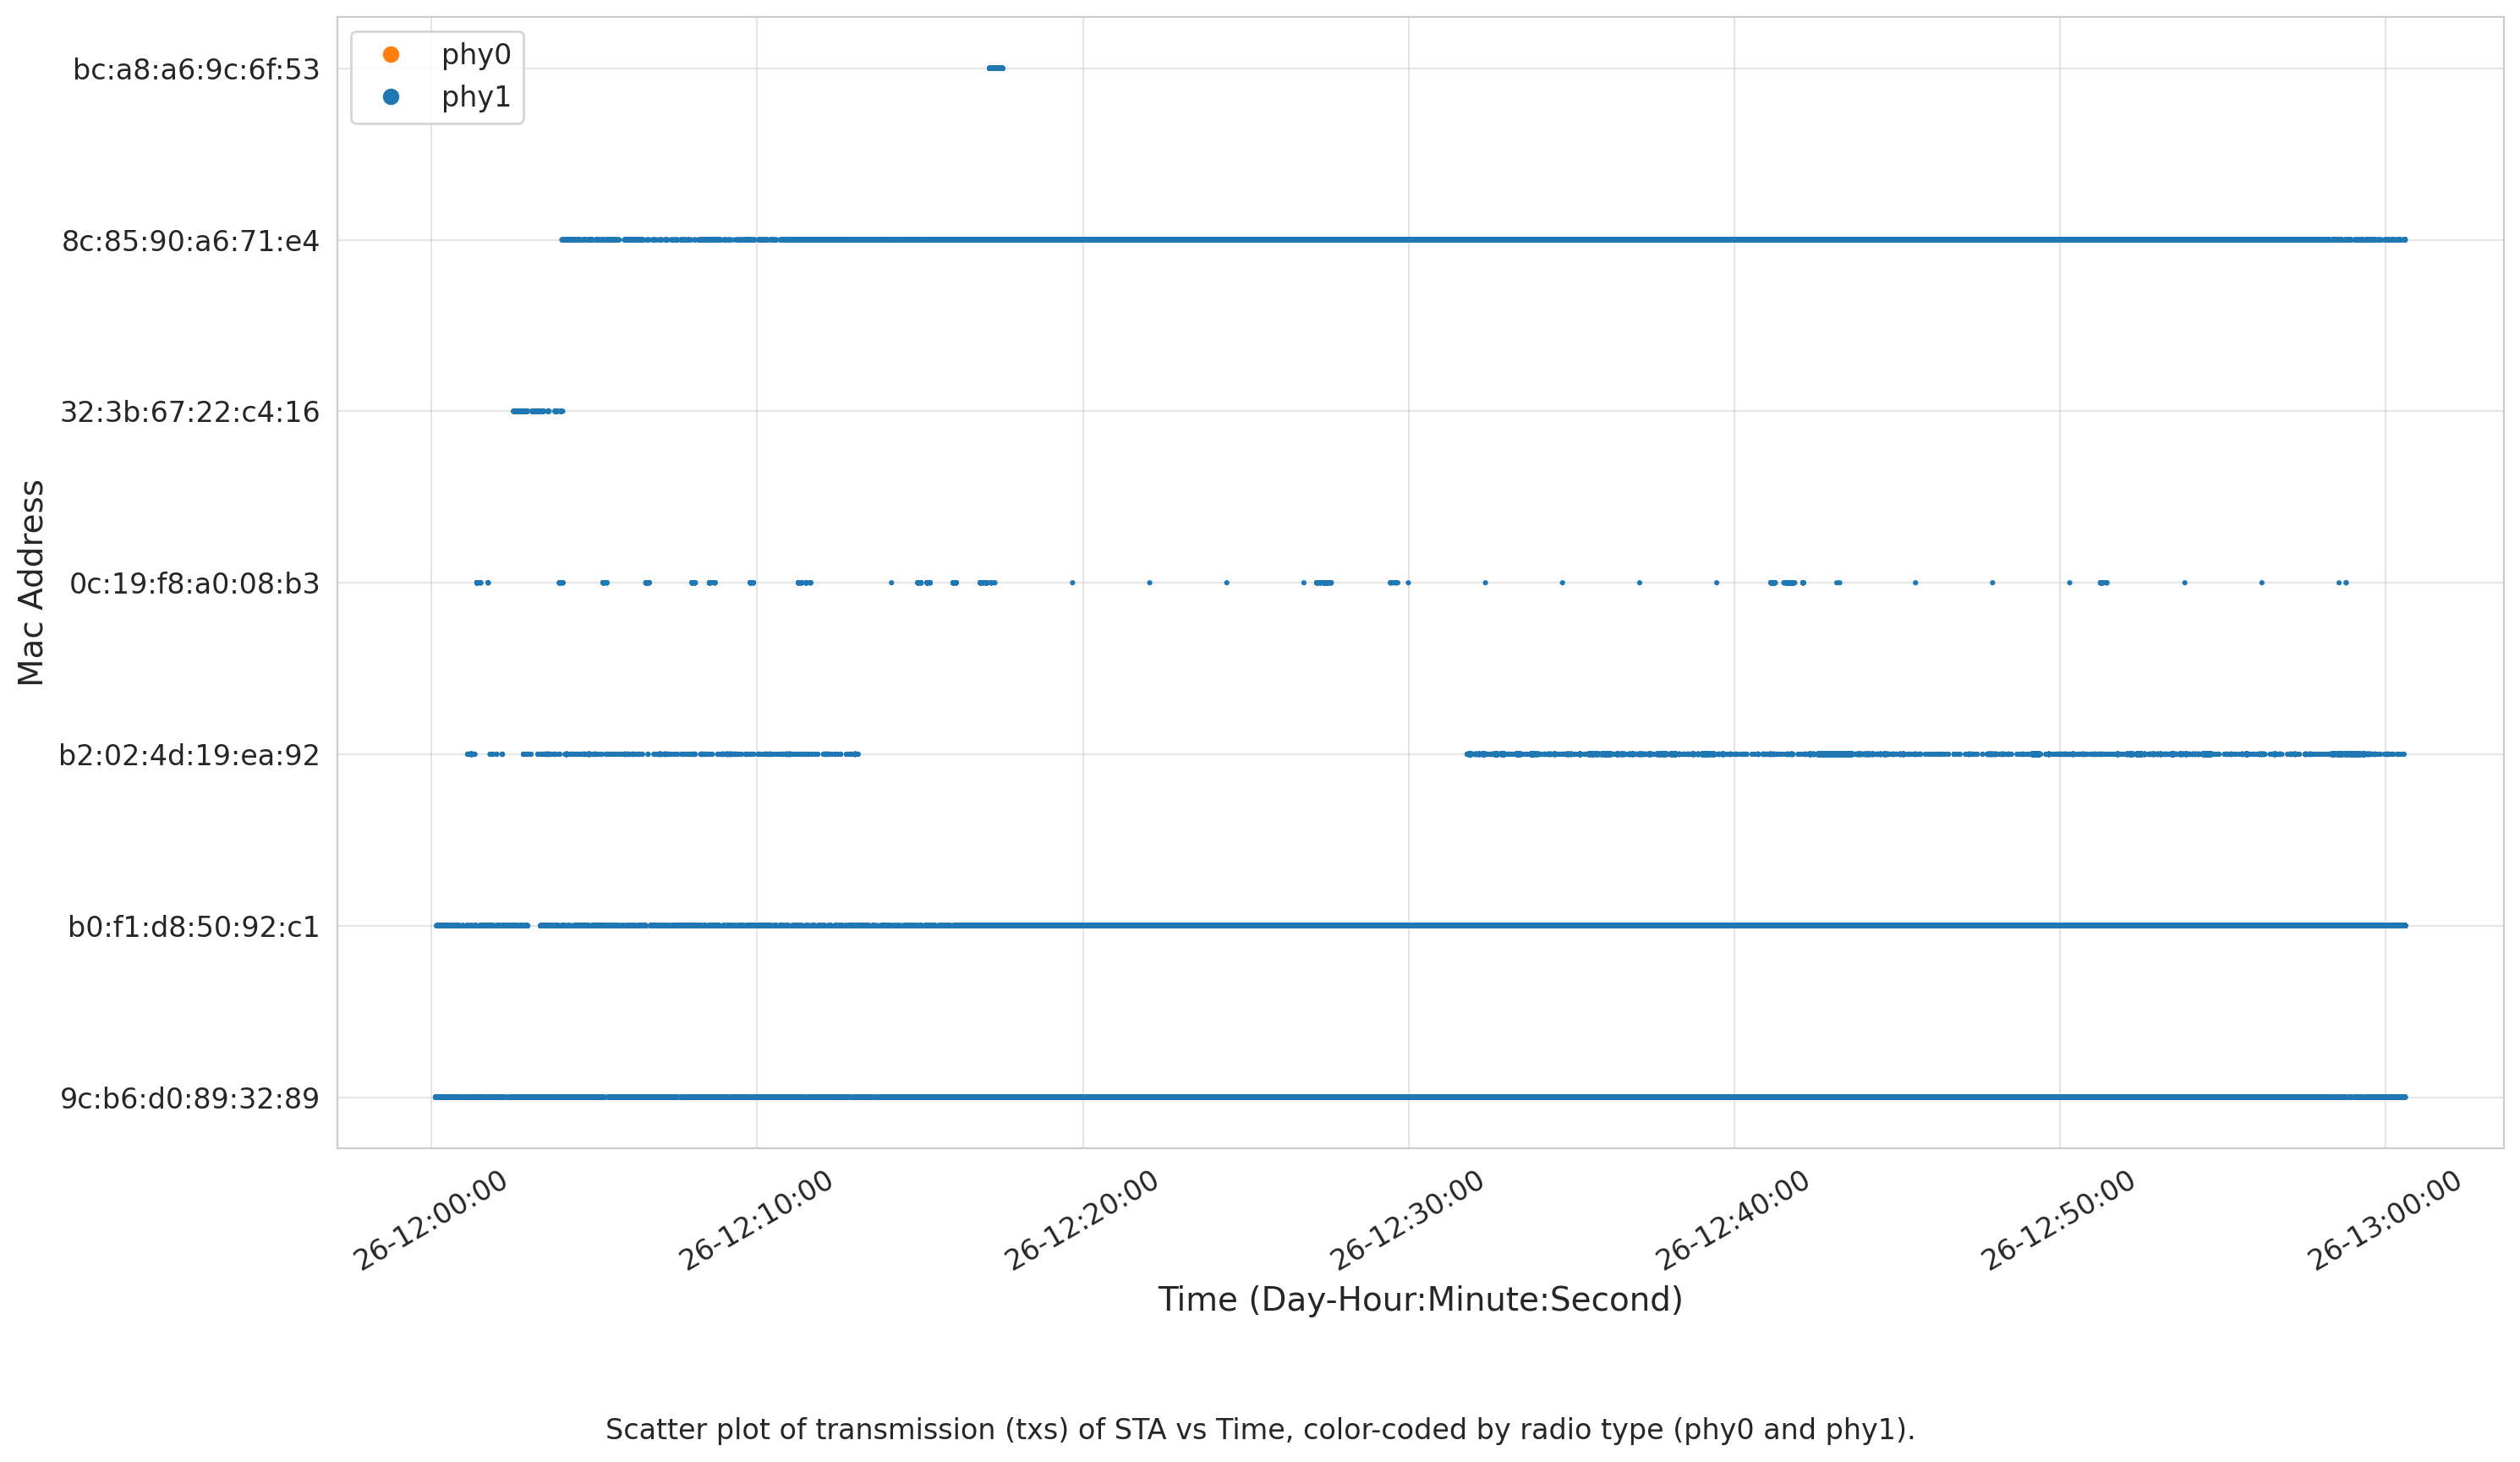
\includegraphics[width=1.45\textwidth, height=\textheight, keepaspectratio]{figures/plots/Scenario-1/G1-22.png}
\caption[Transmission of Stations Over Time]{Scenario-1: Transmission of Stations Over Time: All active stations in the channel are represented by their MAC addresses. The orange color indicates transmission via radio Phy0, while the blue color represents transmission via Phy1.}
  \label{fig:populationmap-1}
\end{figure}
\FloatBarrier 
\end{landscape}


\begin{landscape}
\begin{figure}[hbt!]
  \centering
  \includegraphics[width=1.45\textwidth, height=\textheight, keepaspectratio]{figures/plots/Scenario-1/G1-RSSI-b0:f1:d8:50:92:c1.png}
  \caption[Temporal Analysis of Signal Strength]{Scenario-1: Temporal Analysis of Signal Strength: Signal strength values in dBm over a course of time. Lower values indicate weaker signal strength.}
  \label{fig:rxs-1}
\end{figure}
\FloatBarrier 
\end{landscape}


\begin{figure}[hbt!]
  \centering
  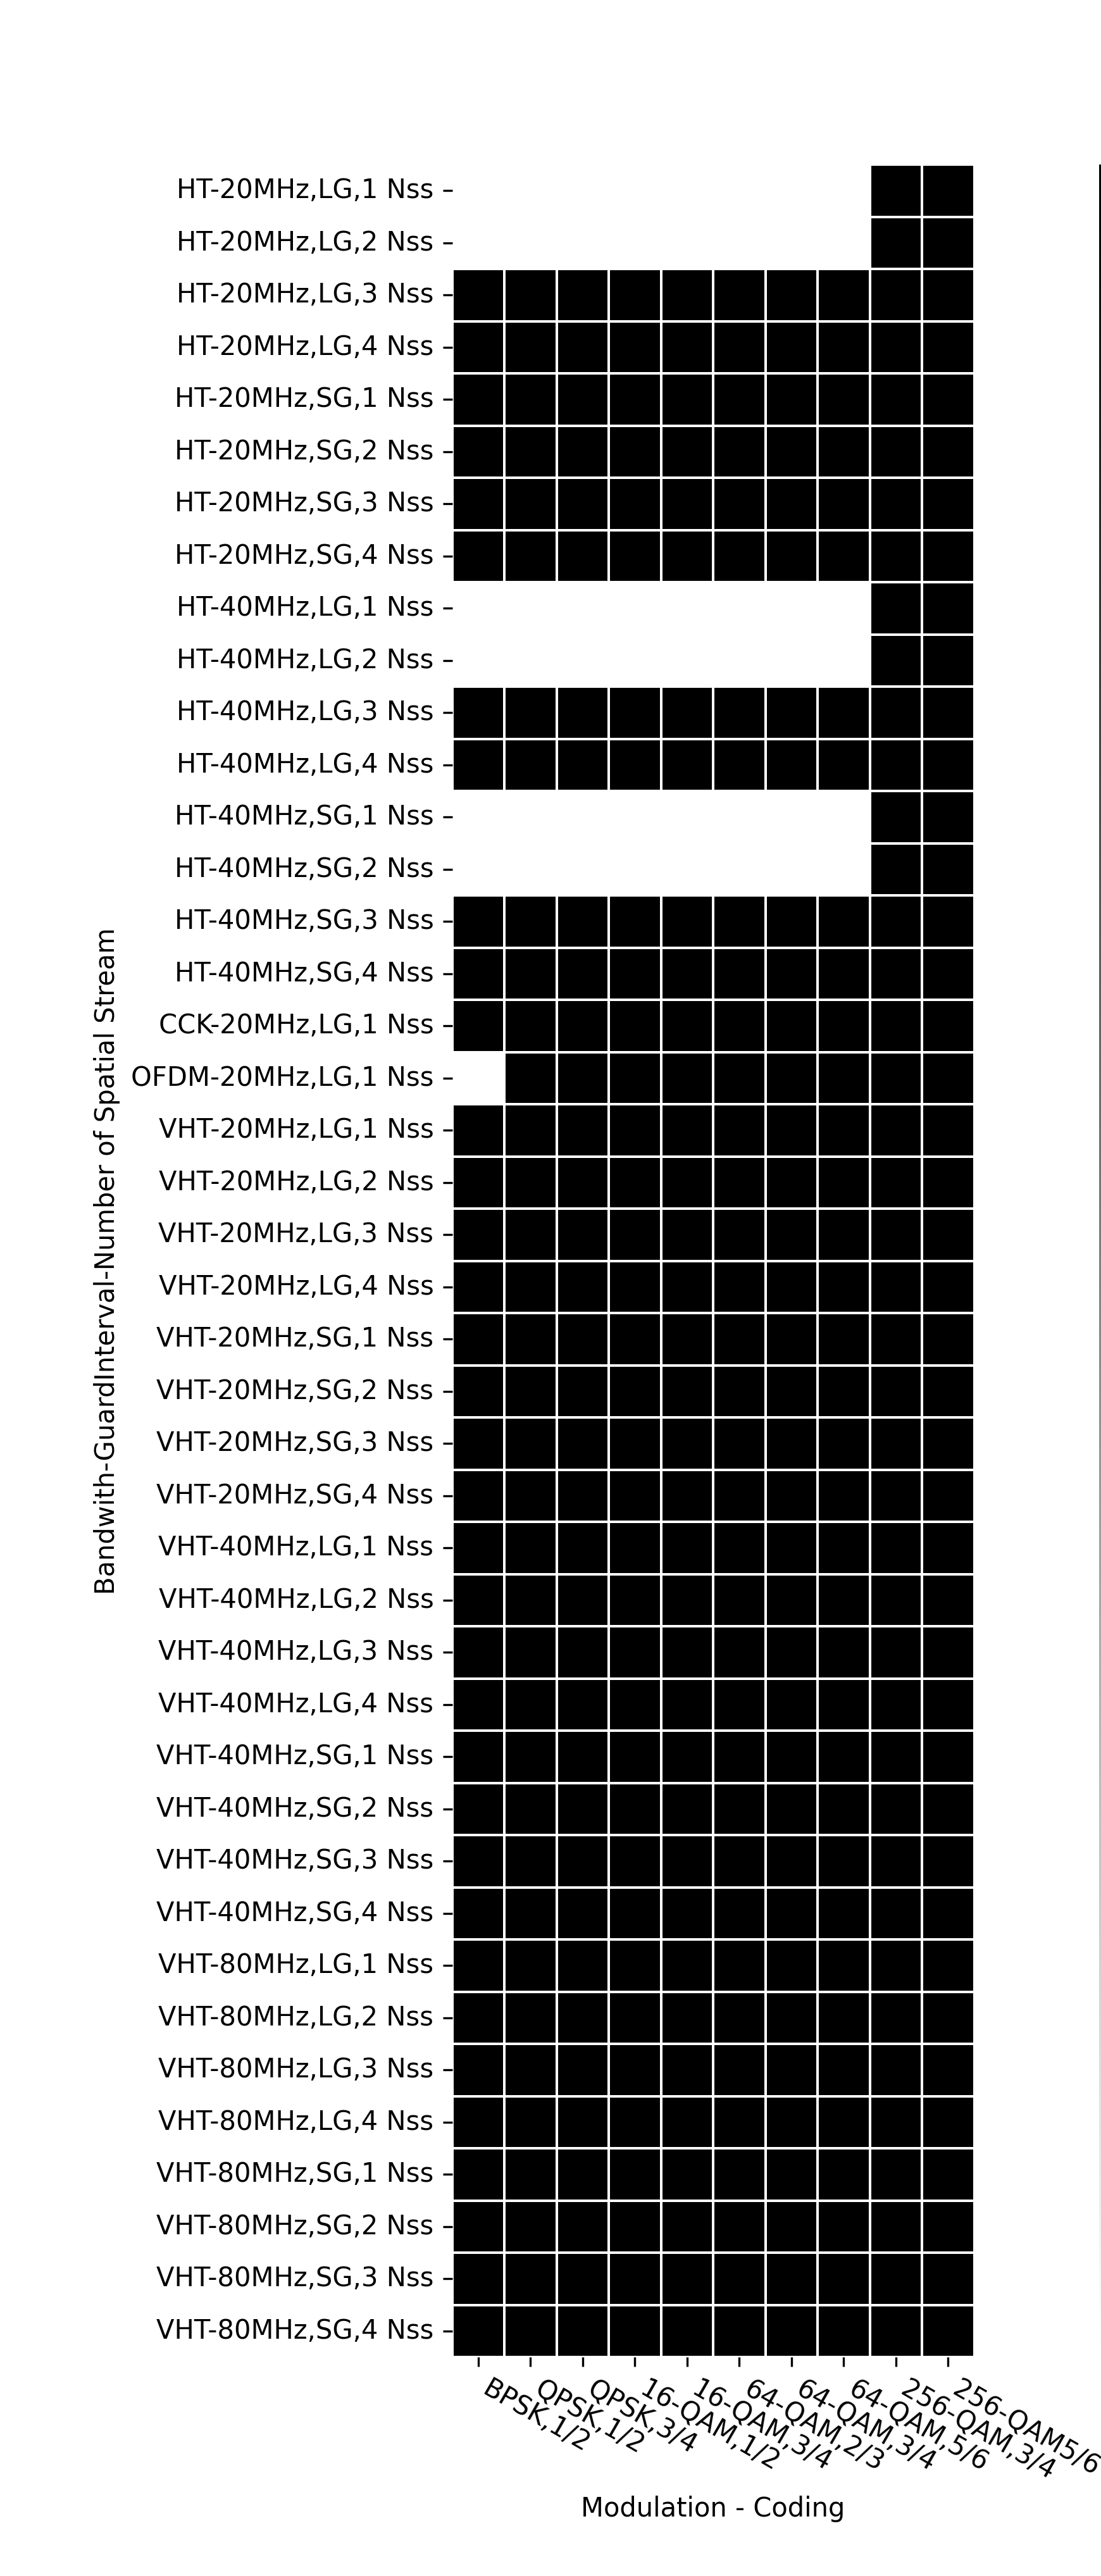
\includegraphics[width=0.5\textwidth]{figures/plots/Scenario-1/G1-invertmap-b0:f1:d8:50:92:c1-22-1652-351697.png}
  \caption[Available rates per station]{White squares represent the available rates for transmitting packets, while black squares indicate unavailable rates for the chip-set of station "b0:f1:d8:50:92:c1".}
  \label{fig:STA}
\end{figure}
\FloatBarrier 


\begin{figure}[hbt!]
  \centering
  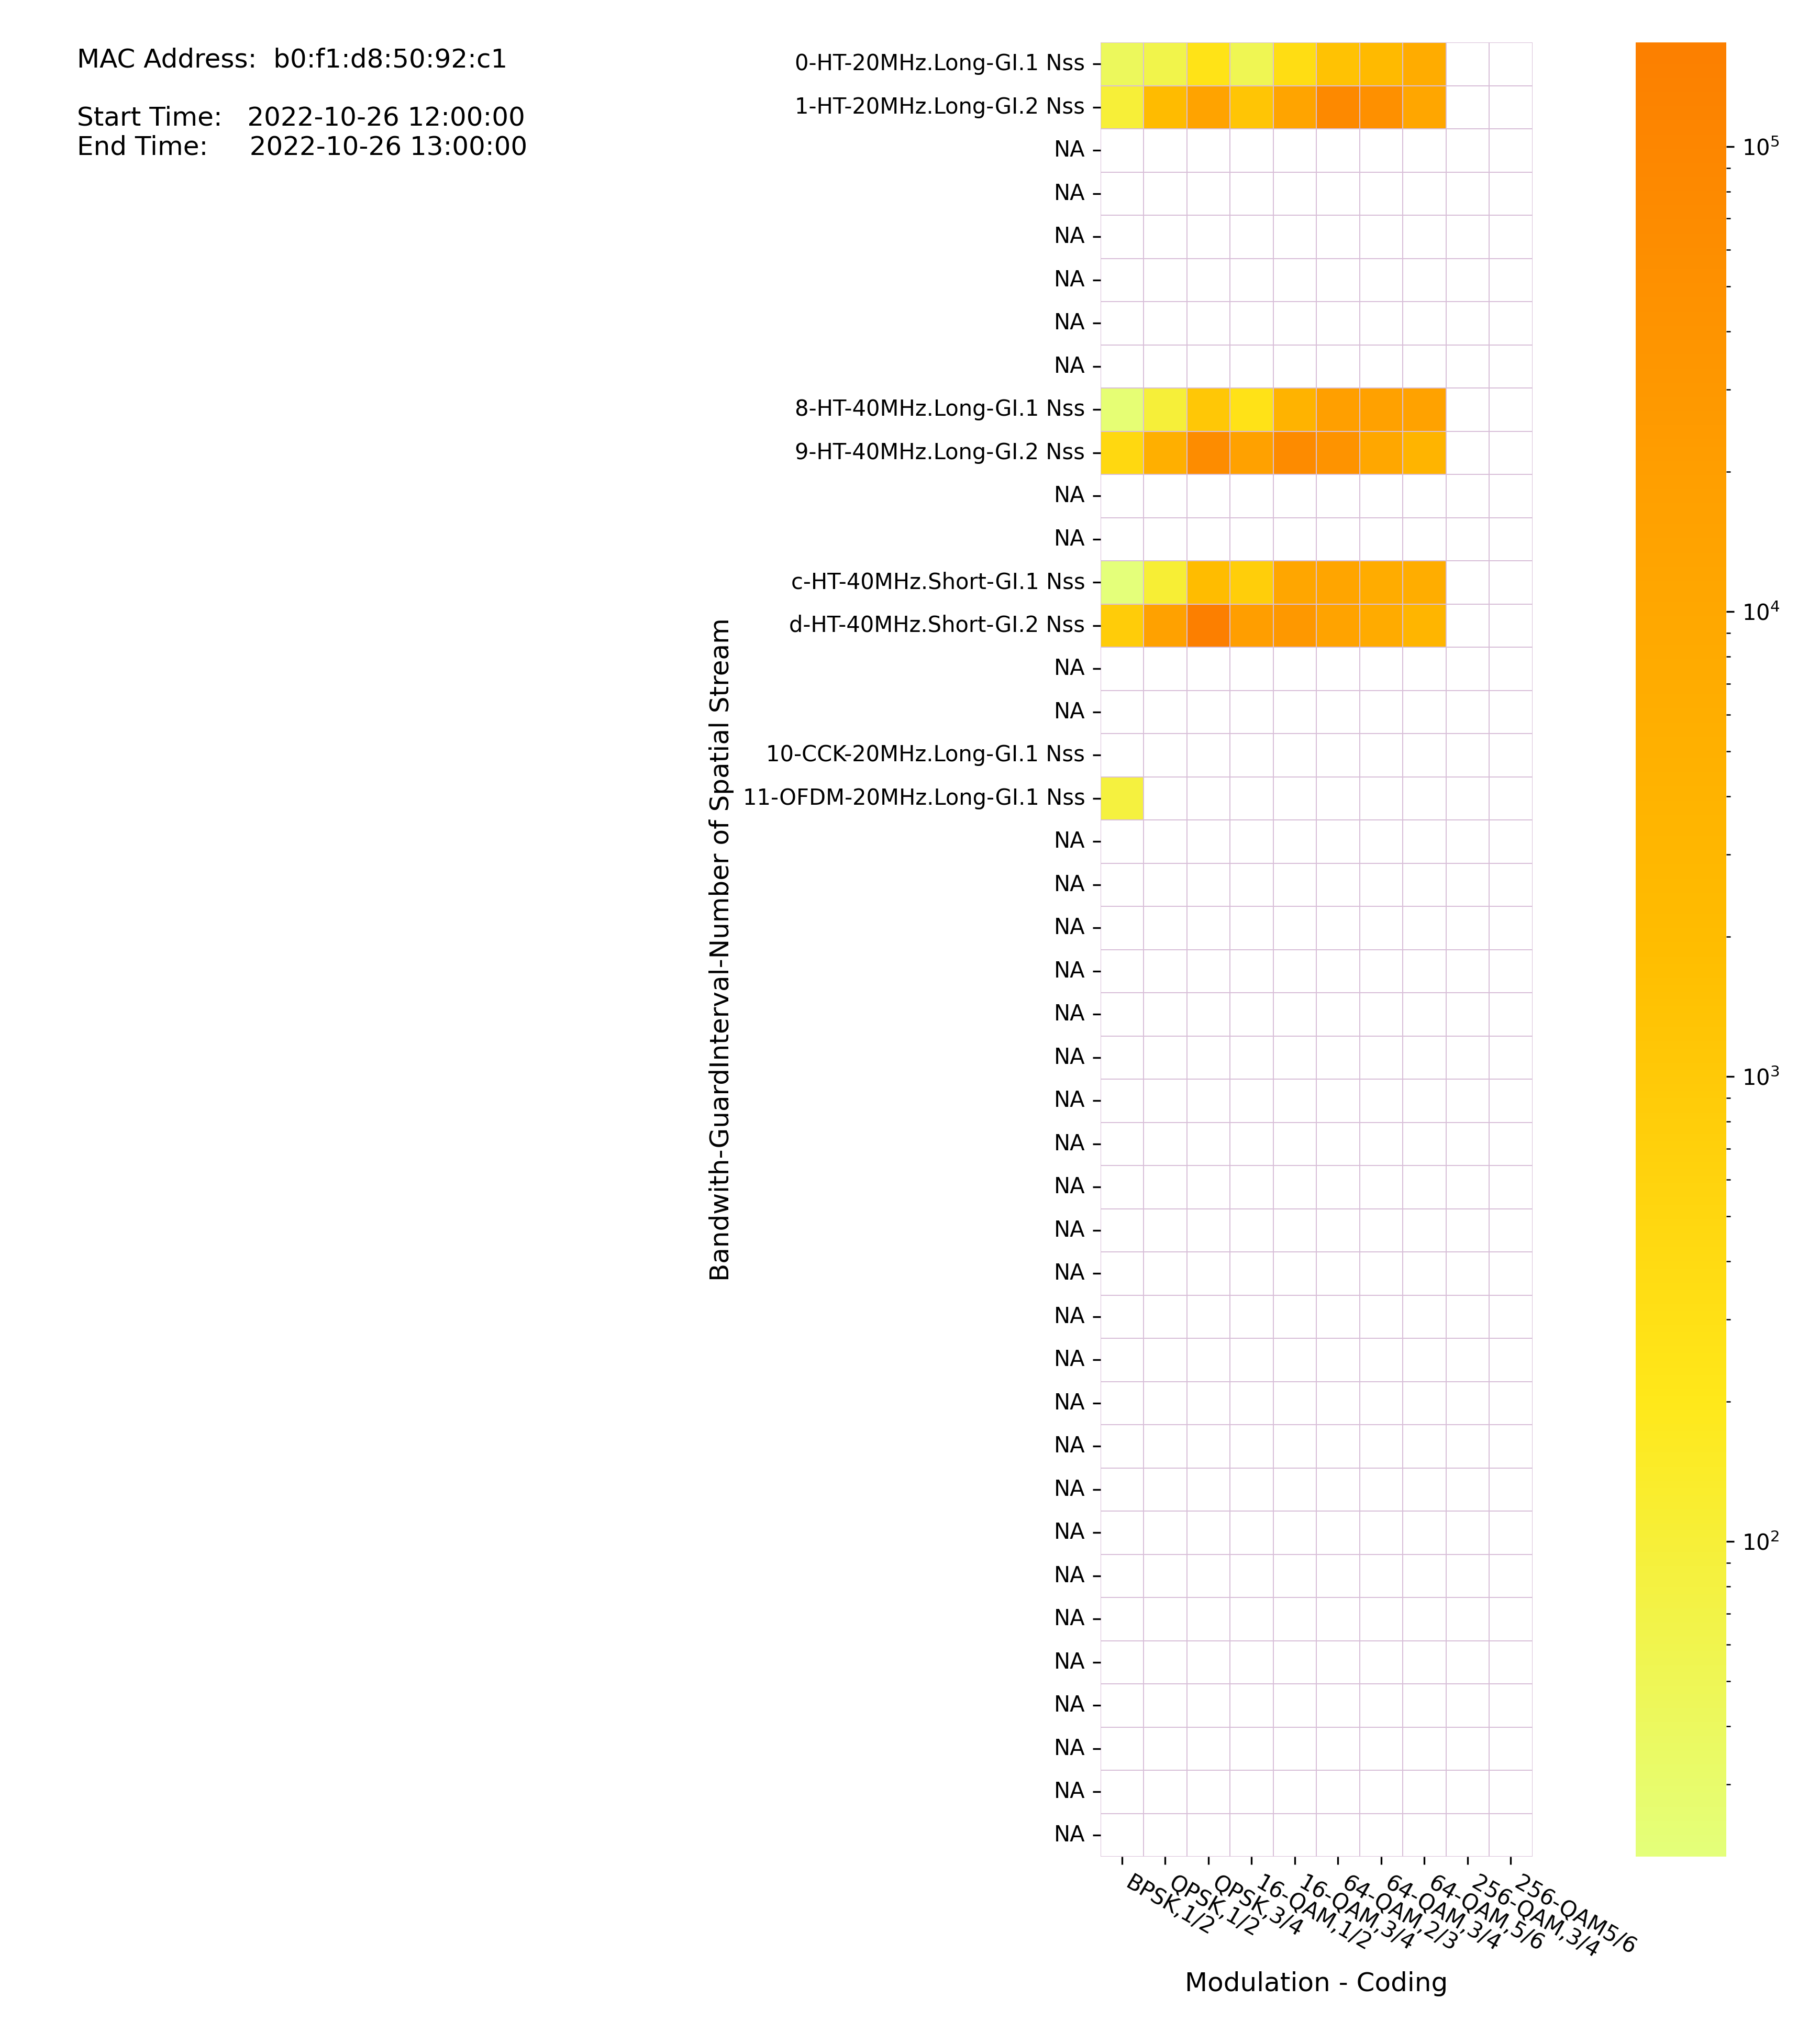
\includegraphics[width=\textwidth]{figures/plots/Scenario-1/G1-attemptmap-b0:f1:d8:50:92:c1-22-1652-351697.png}
  \caption[Transmission Status]{Scenario-1: Transmitted rates per rates group index over Modulation and Coding. The colorbar represents the number of transmitted packets (ACK and Non-Ack). The start and end times of observation, as well as the MAC address of the station, are indicated in the plot.}
  \label{fig:Attempt1}
\end{figure}
\FloatBarrier 


\begin{figure}[hbt!]
  \centering
  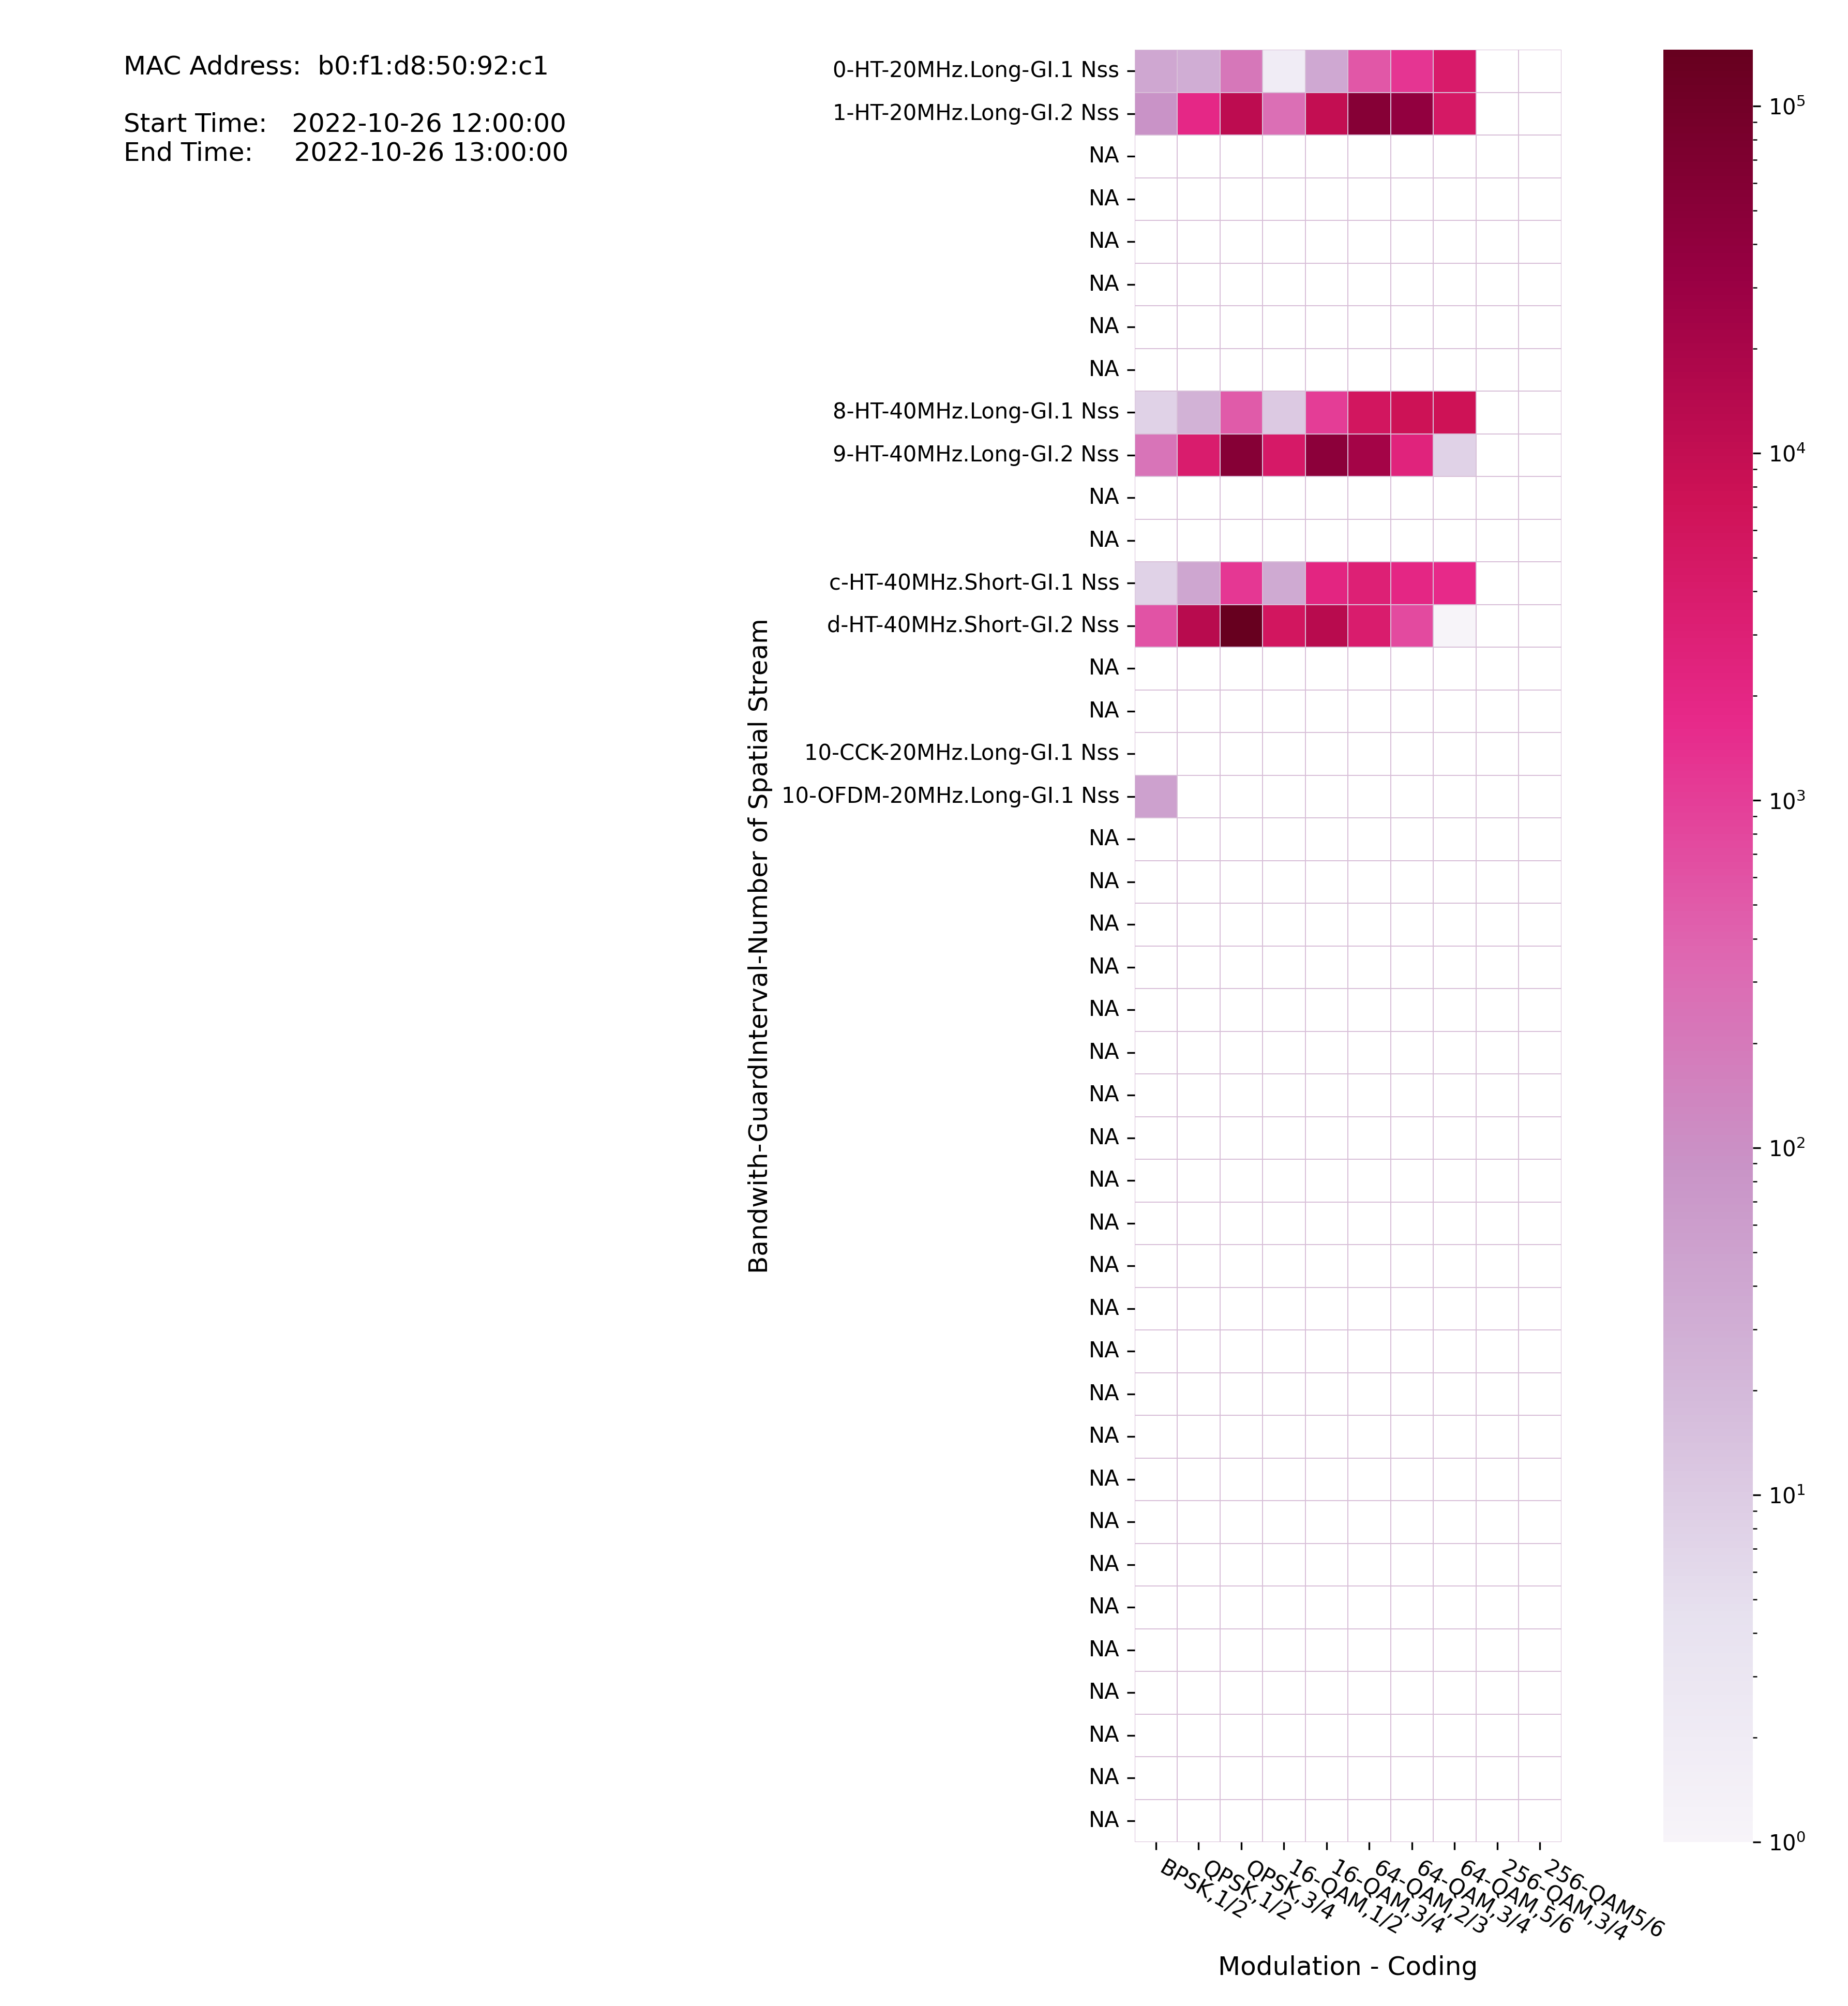
\includegraphics[width=\textwidth]{figures/plots/Scenario-1/G1-heatmap-b0:f1:d8:50:92:c1-22-1652-351697.png}
  \caption[Rate-Based Packet Success Analysis]{Scenario-1: Successfully transmitted rates per rates group index over Modulation and Coding. The colorbar represents the number of successfully transmitted packets (ACK). The start and end times of observation, as well as the MAC address of the station, are indicated in the plot.}
  \label{fig:Success-count1}
\end{figure}
\FloatBarrier 


\begin{figure}[hbt!]
  \centering
  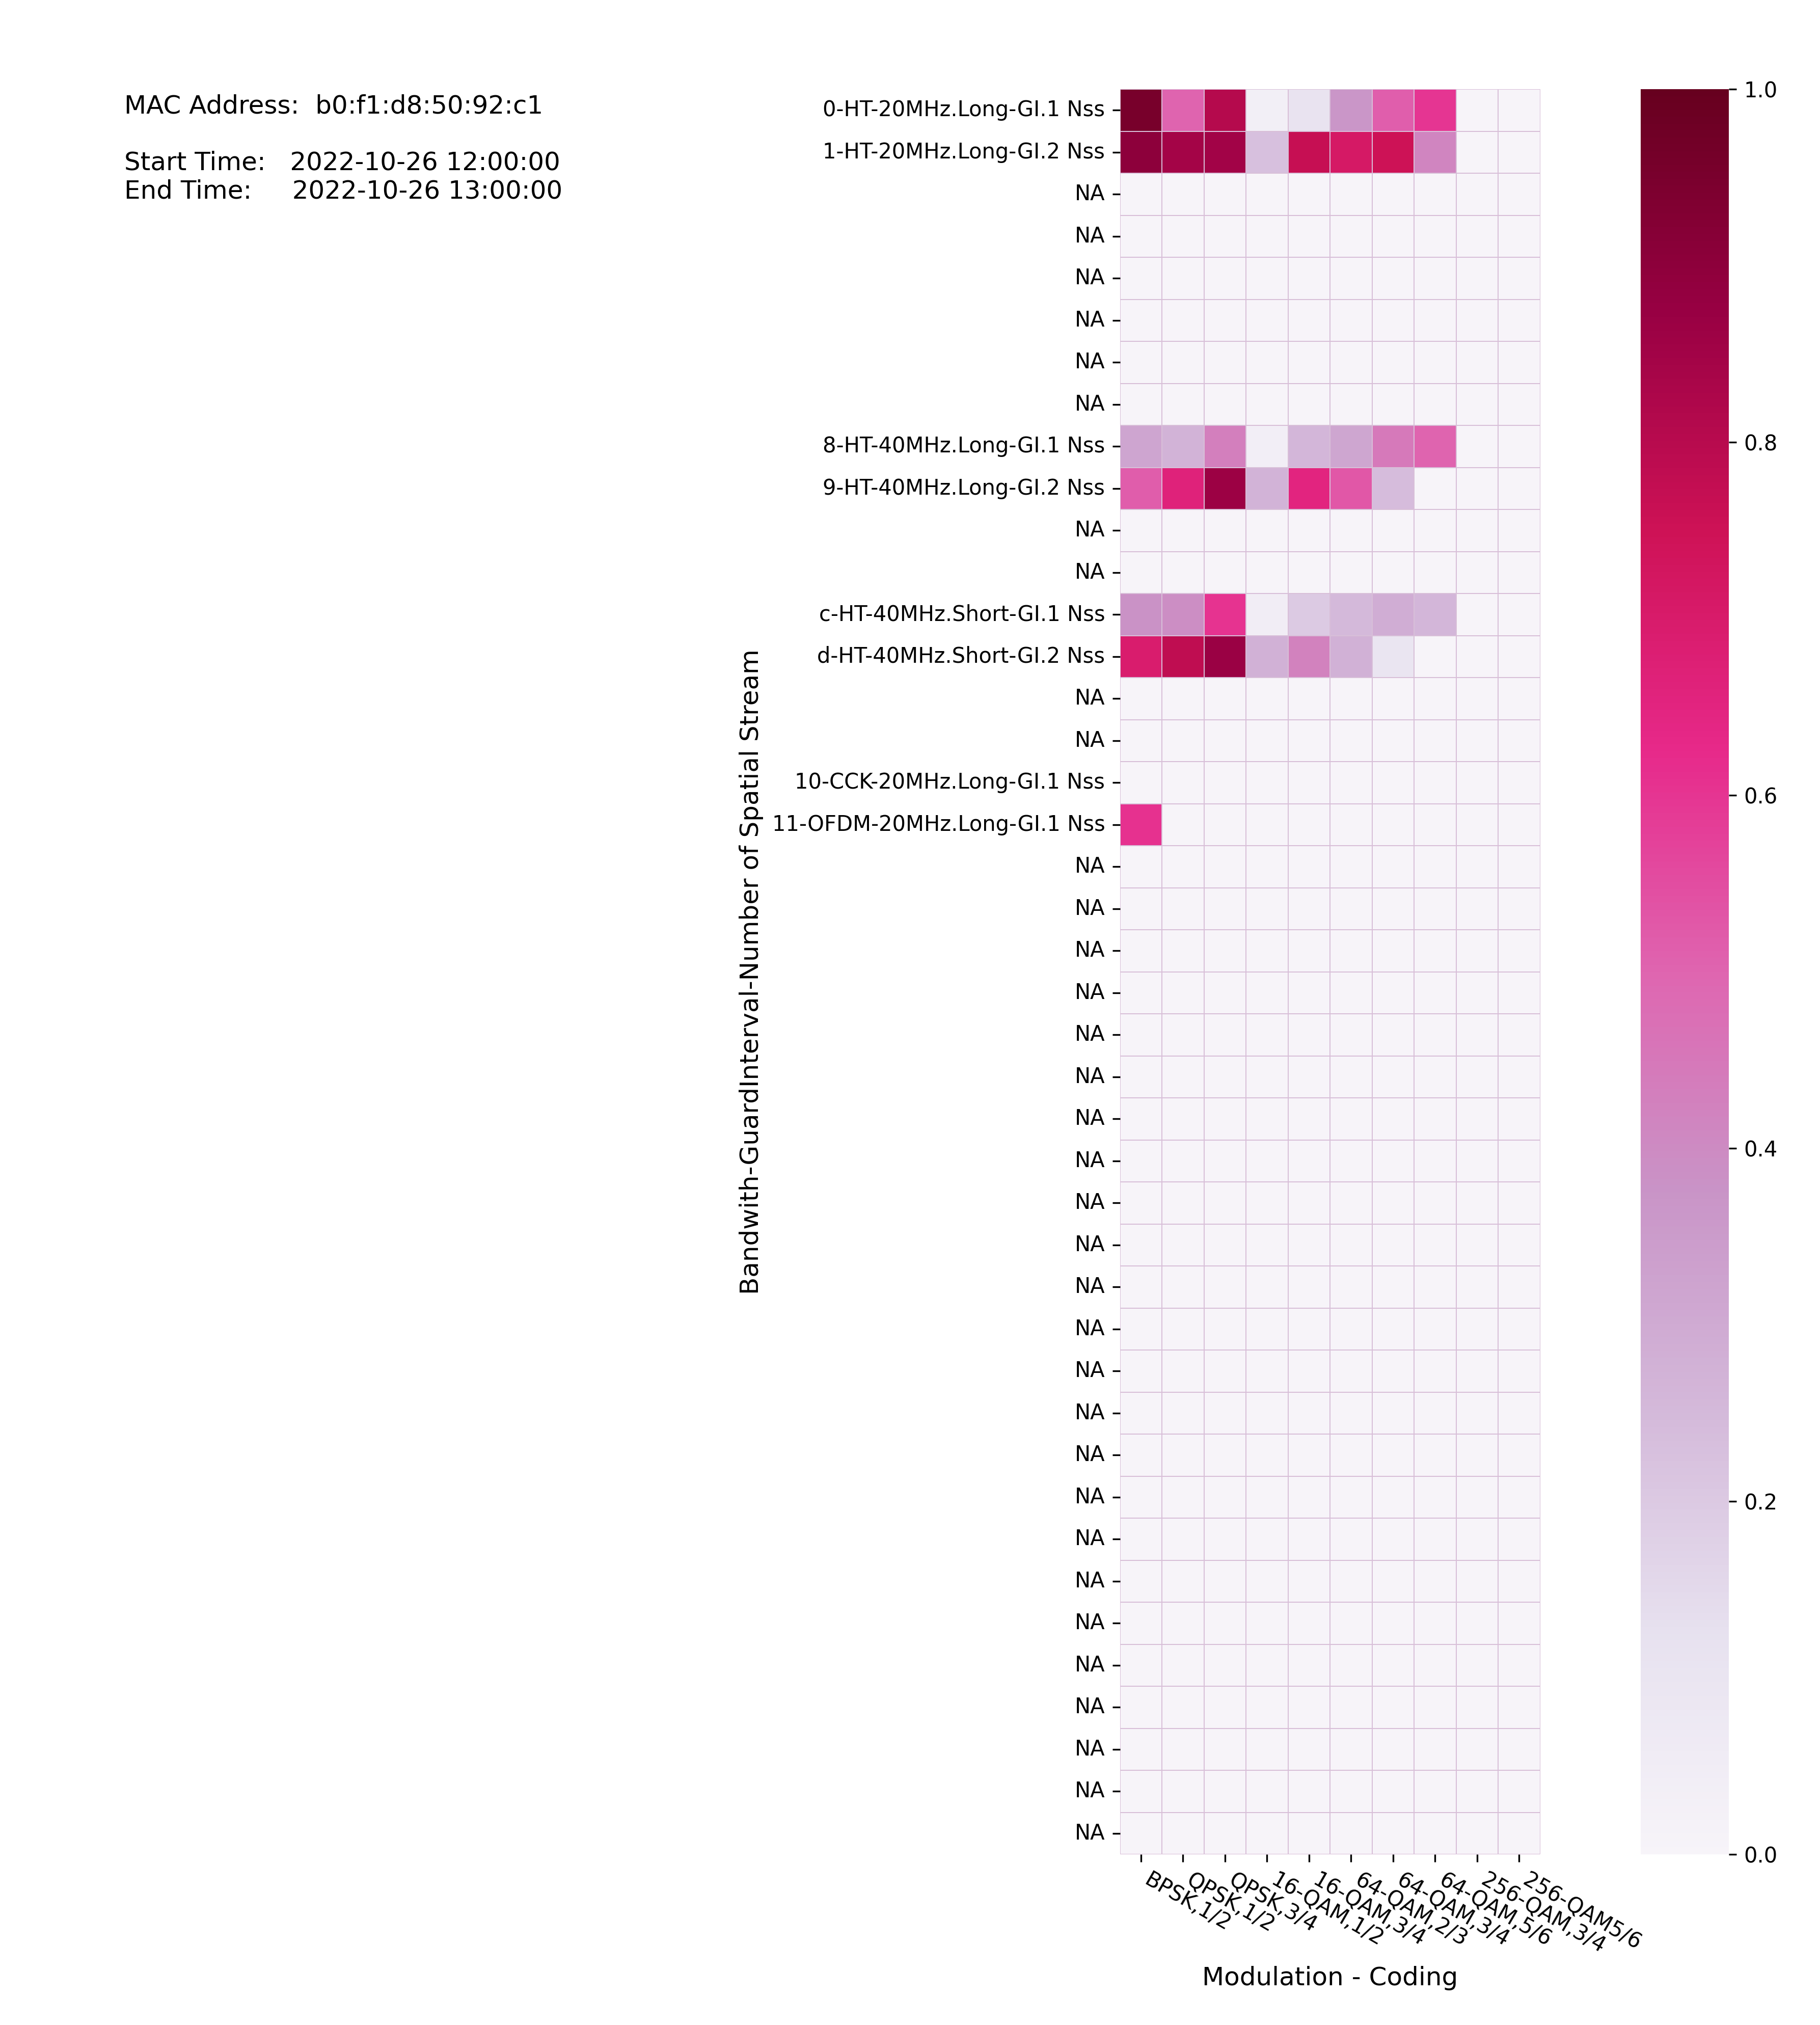
\includegraphics[width=\textwidth]{figures/plots/Scenario-1/G1-heatmap-p-b0:f1:d8:50:92:c1-22-1652-351697.png}
  \caption[Probability of Success for Rate-Based Transmission]{Scenario-1: Probability of successfully transmitted rates per rates group index over Modulation and Coding. The colorbar represents the probability scaled from 0 to 1.}
  \label{fig:Success-probability1}
\end{figure}
\FloatBarrier 

\begin{landscape}
\begin{figure}[hbt!]
  \centering
  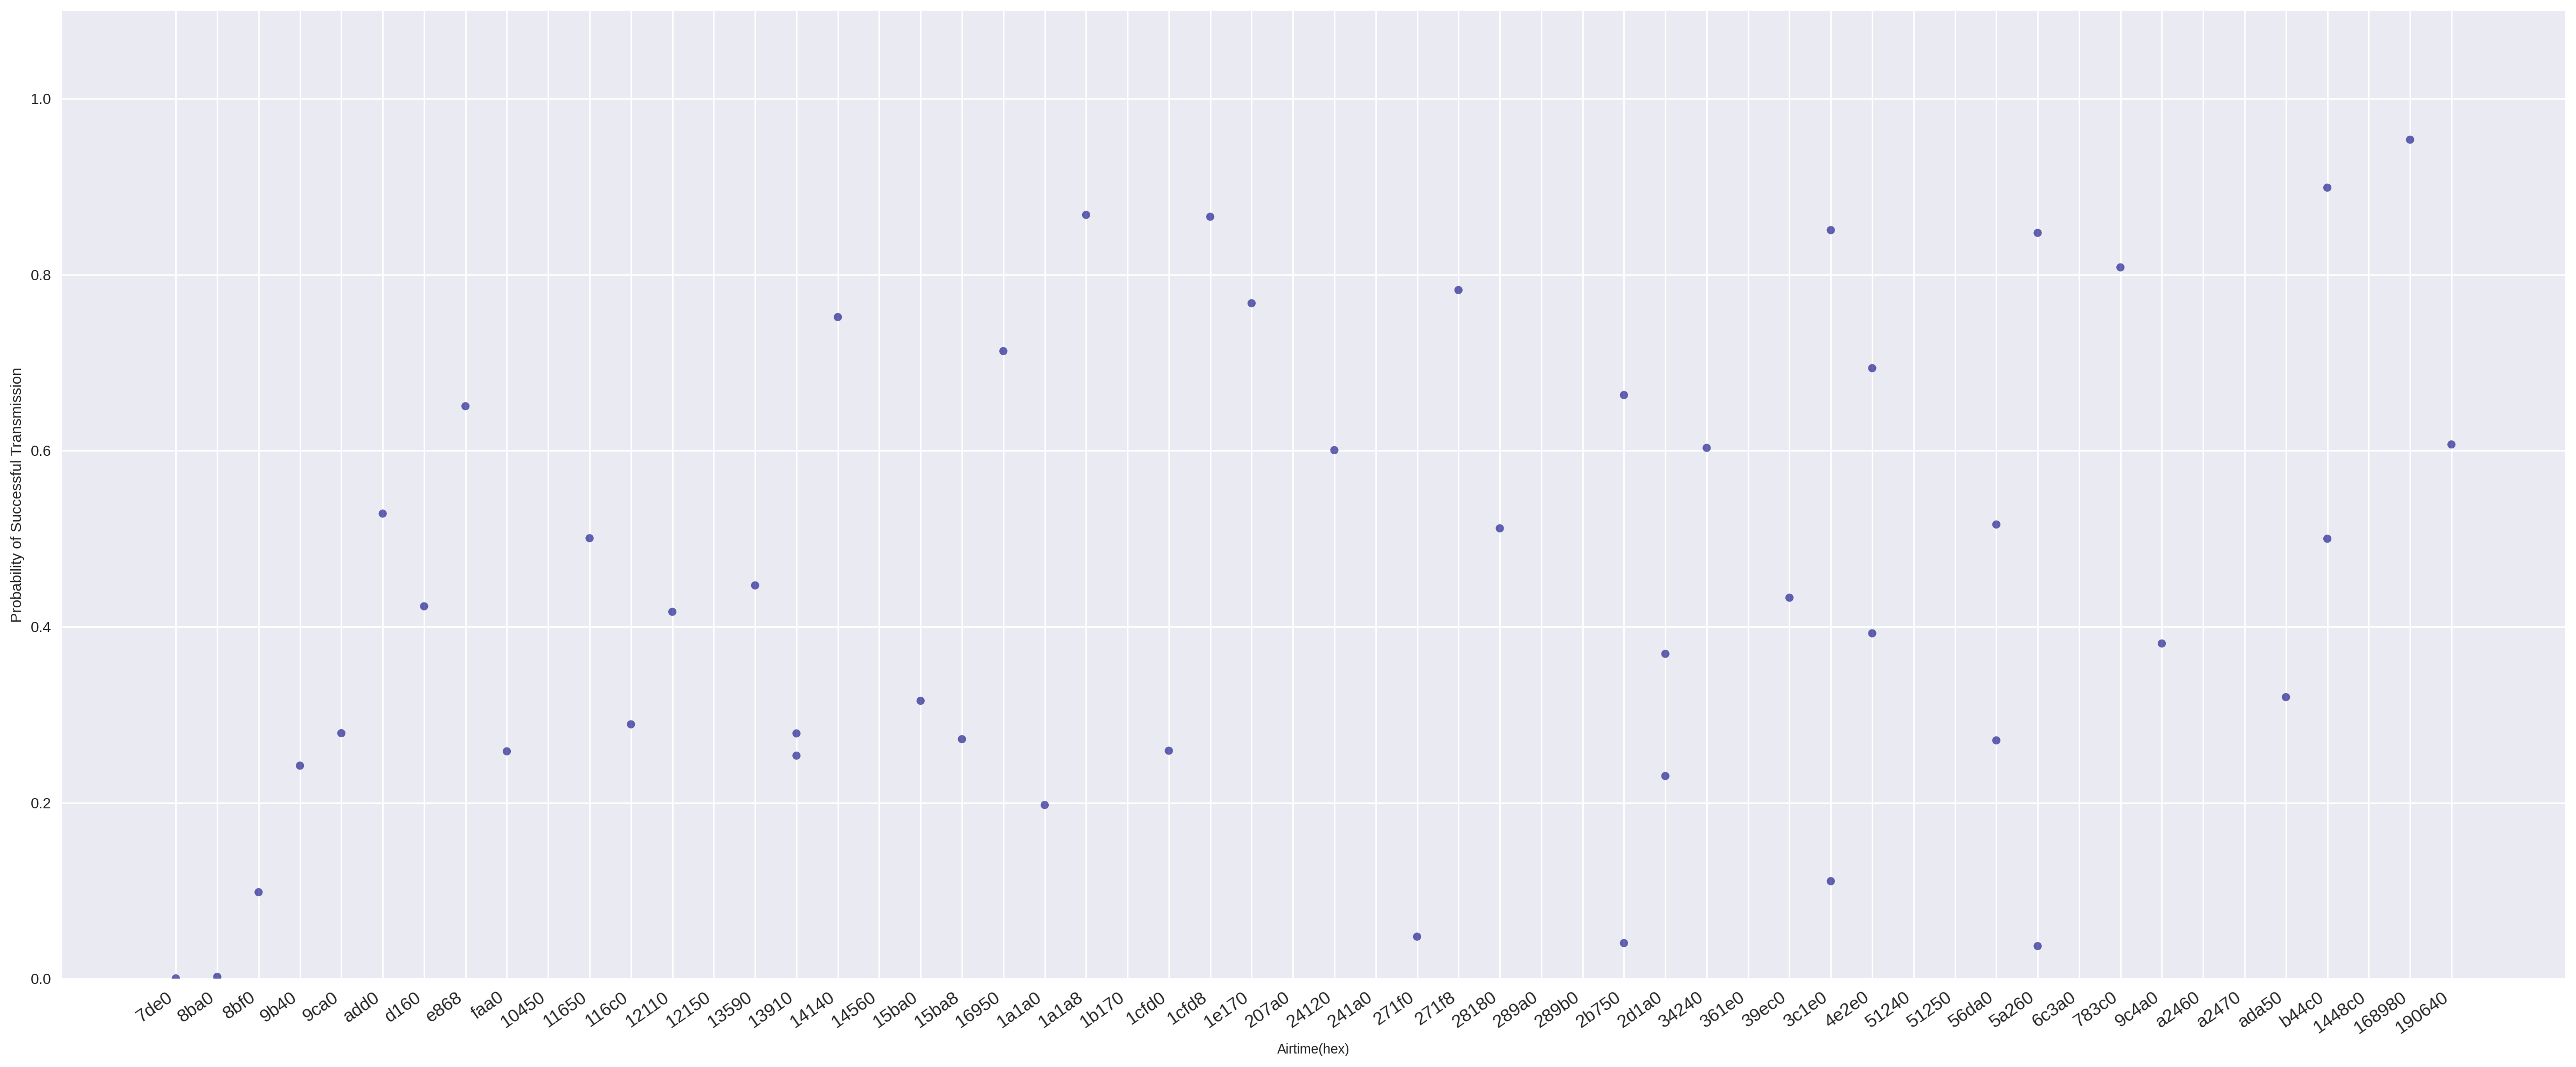
\includegraphics[width=1.45\textwidth, height=\textheight, keepaspectratio]{figures/plots/Scenario-1/G1-probability vs airtime-b0:f1:d8:50:92:c1-22-1652-351697.png}
  \caption[Airtime-Based Success Probability for Rate-Based Transmission]{Scenario-1: Airtime values in nanoseconds (hex notation) on the x-axis, and the probability of success on the y-axis.}
  \label{fig:Success-p-vs-airtime1}
\end{figure}
\FloatBarrier 
\end{landscape}

\begin{figure}[hbt!]
  \centering
  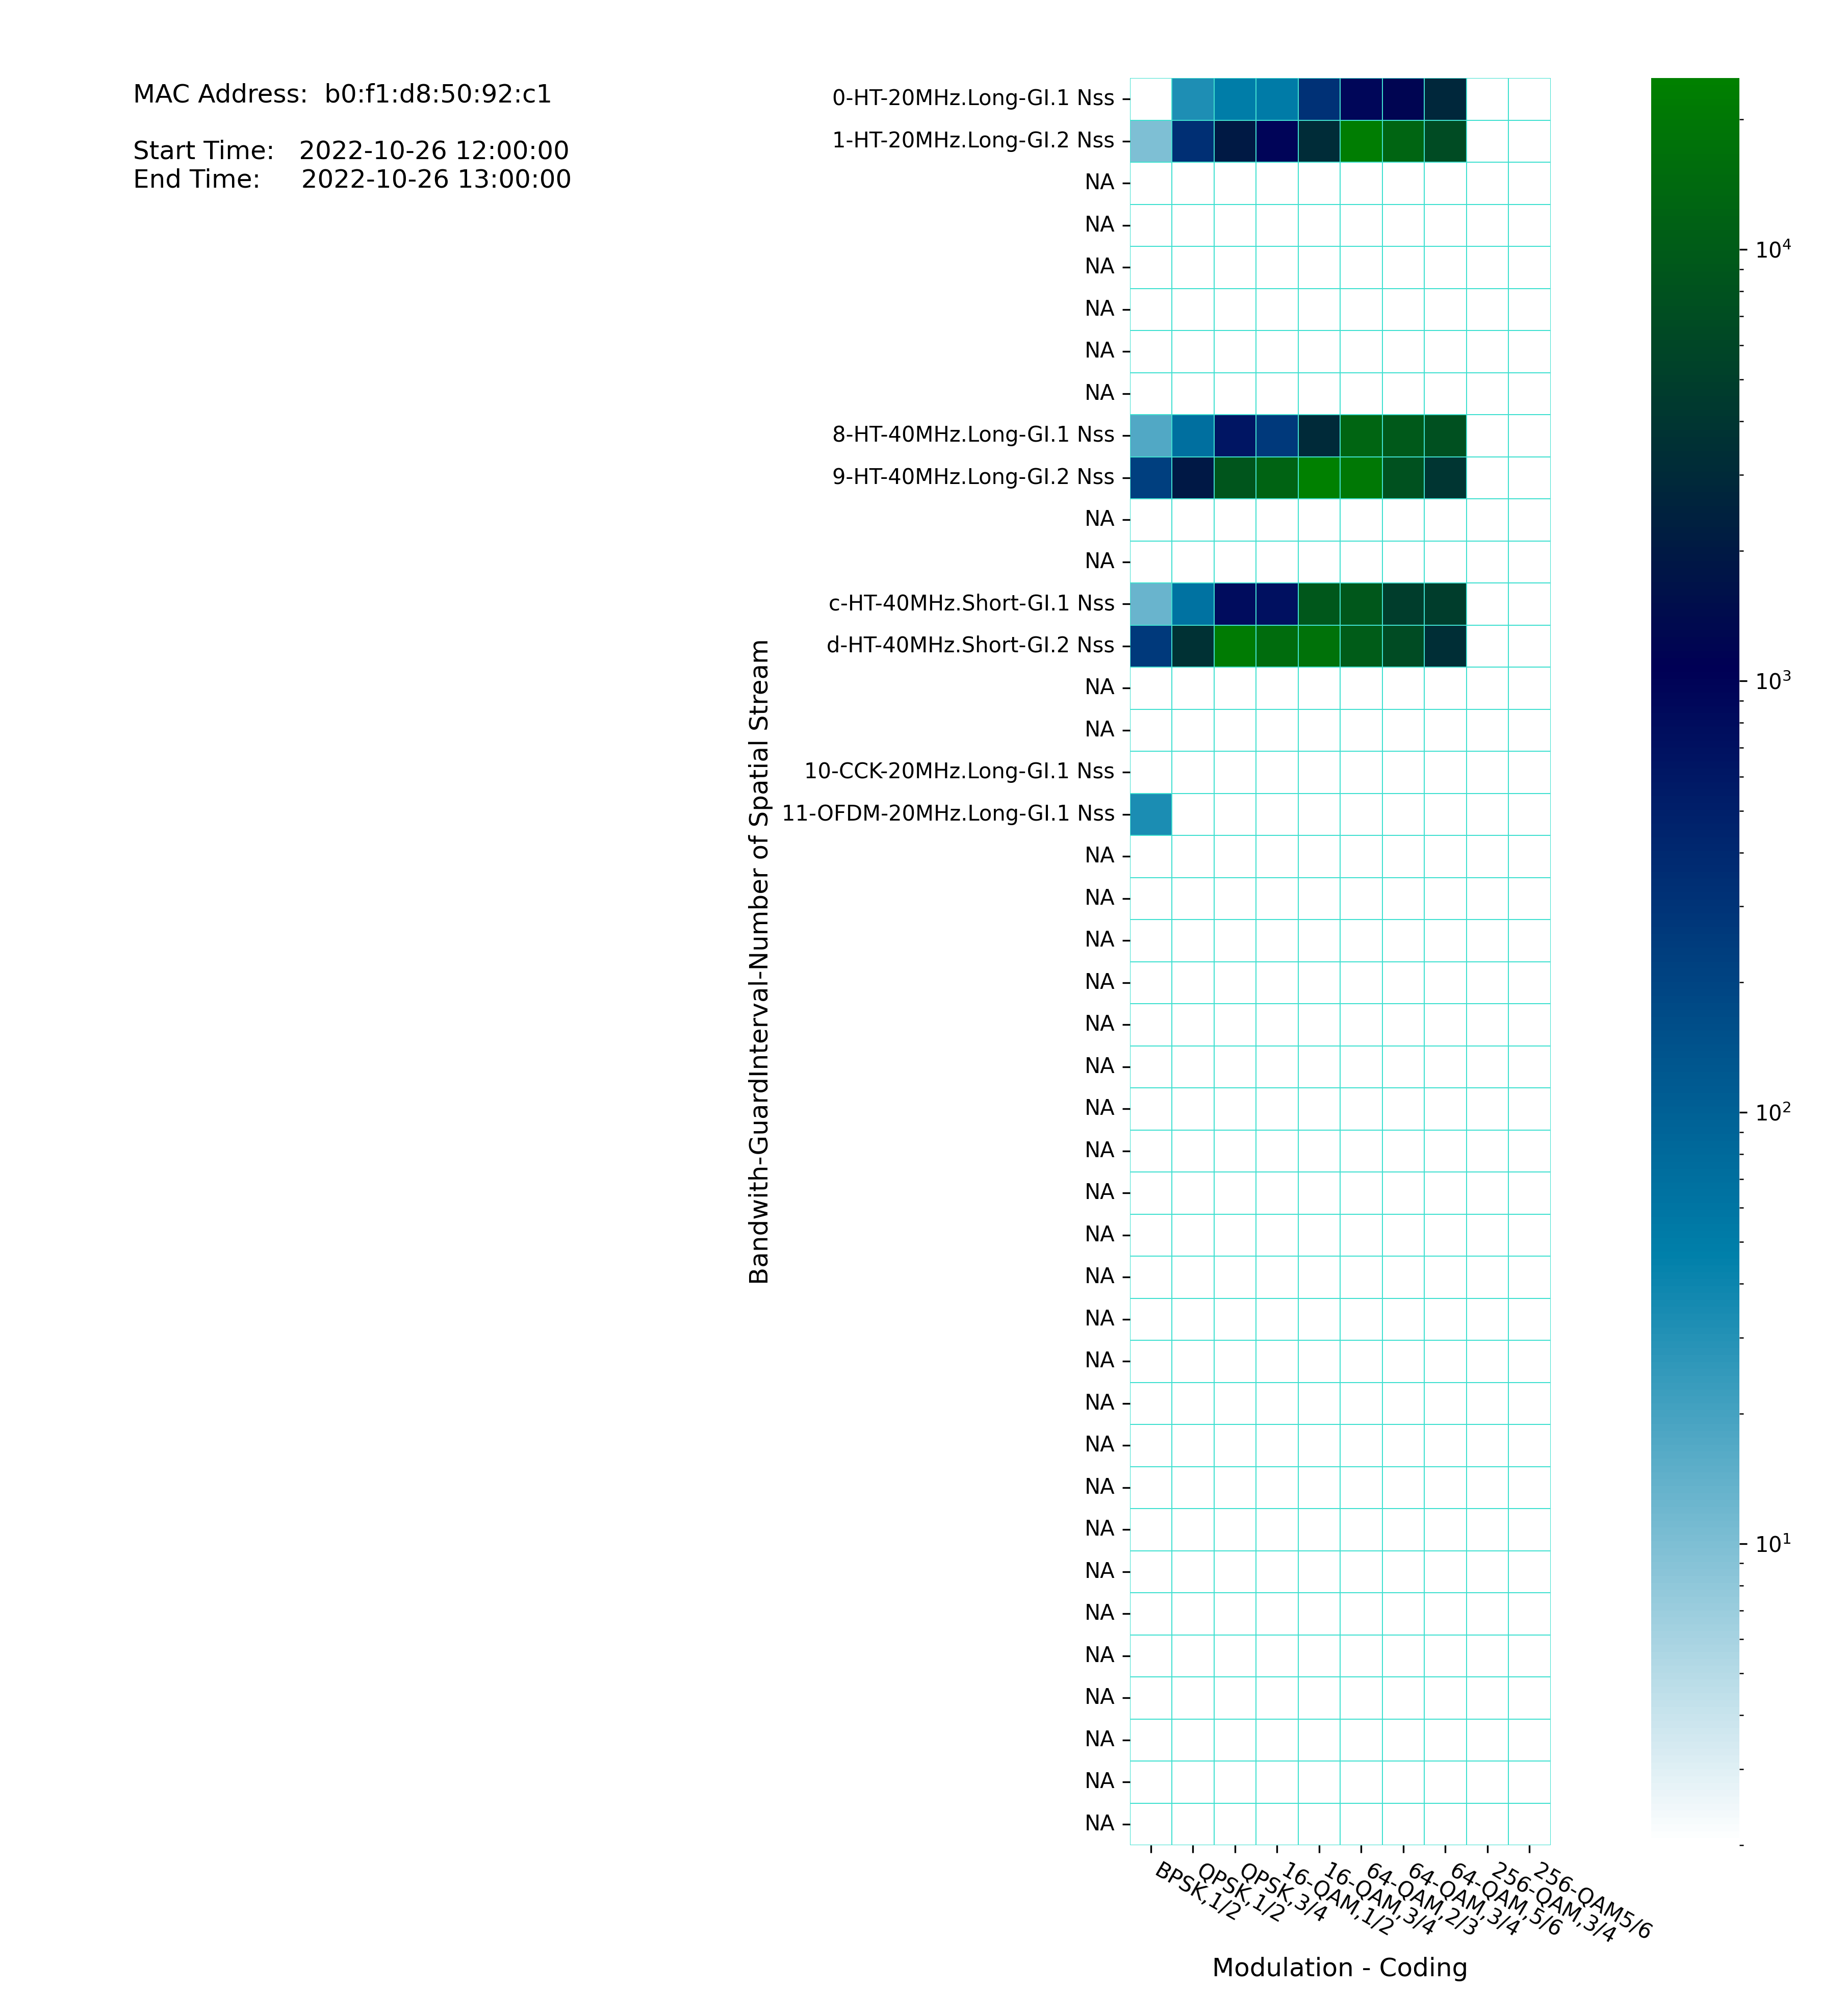
\includegraphics[width=\textwidth]{figures/plots/Scenario-1/G1-coldmap-b0:f1:d8:50:92:c1-22-1652-351697.png}
  \caption[Rate-Based Packet Failure Analysis]{Scenario-1: Failed transmitted rates per rates group index over Modulation and Coding. The colorbar represents the number of failed transmitted packets (Non-ACK). The start and end times of observation, as well as the MAC address of the station, are indicated in the plot.}
  \label{fig:Fail-count1}
\end{figure}
\FloatBarrier 

\begin{figure}[hbt!]
  \centering
  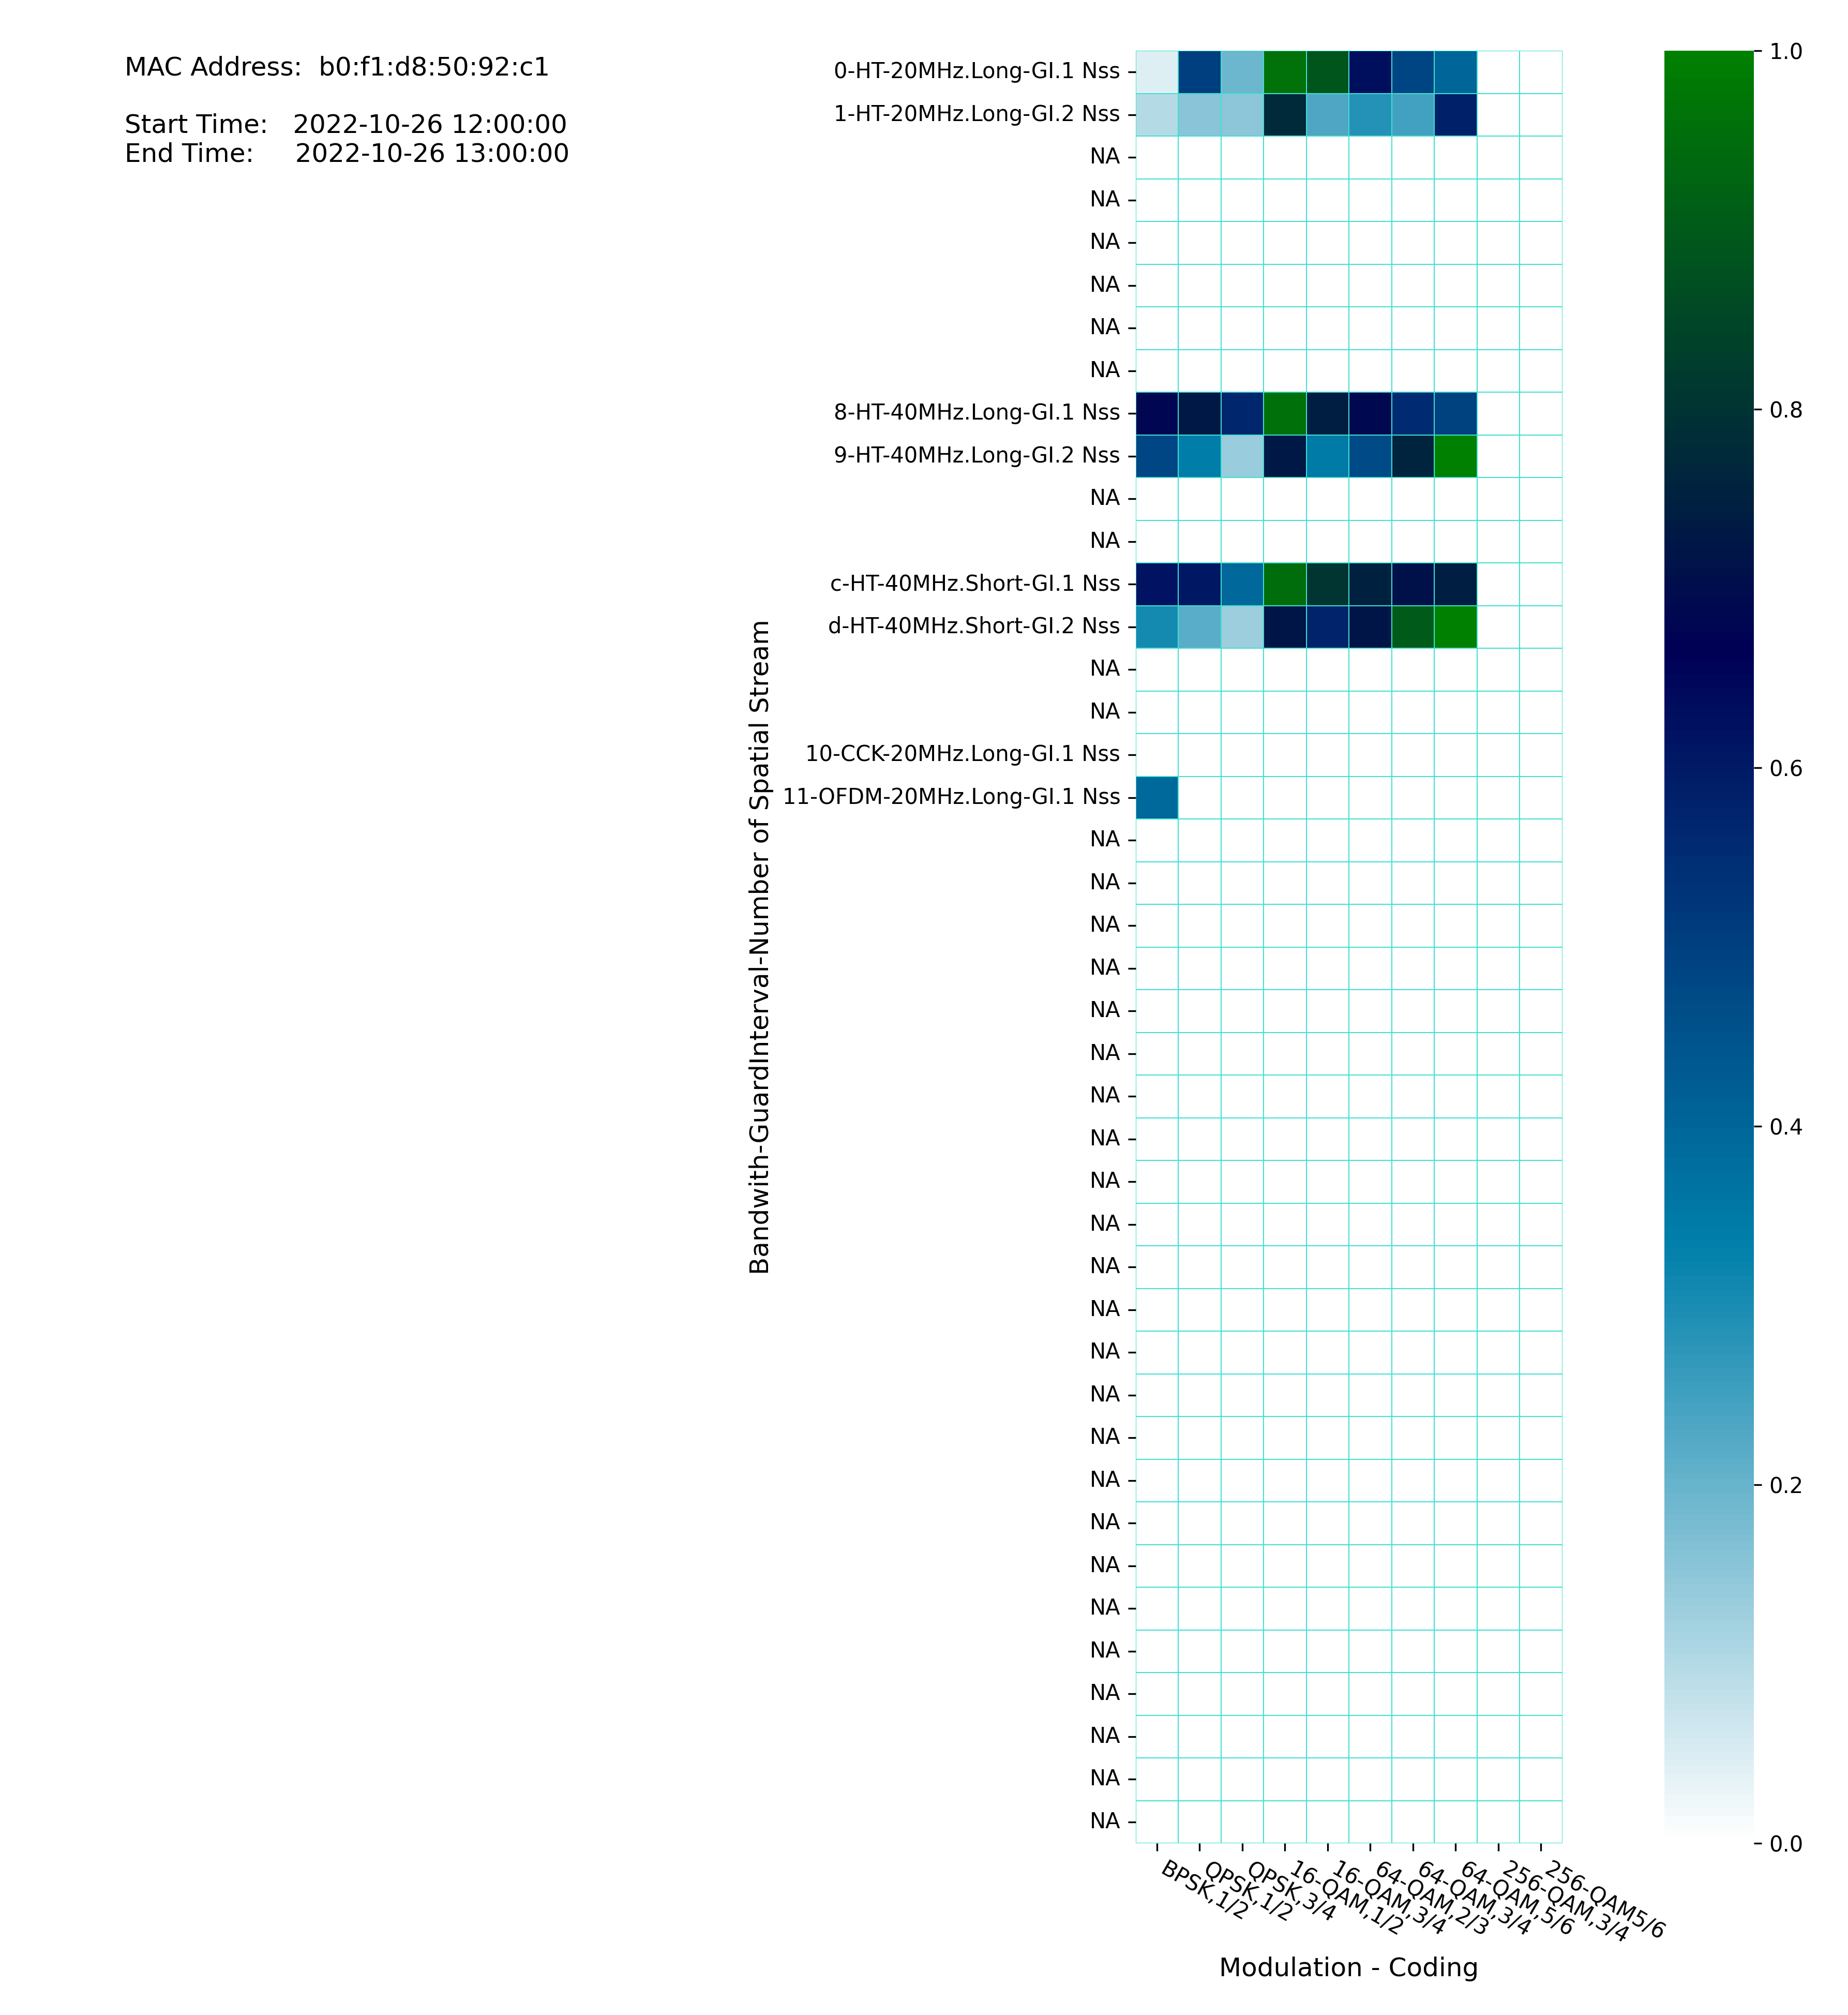
\includegraphics[width=\textwidth]{figures/plots/Scenario-1/G1-coldmap-p-b0:f1:d8:50:92:c1-22-1652-351697.png}
  \caption[Rate-Based Transmission Failure Analysis]{Scenario-1: Probability of failed transmitted rates per rates group index over Modulation and Coding. The colorbar represents the probability scaled from 0 to 1.}
  \label{fig:Fail-probability1}
\end{figure}
\FloatBarrier 

\begin{landscape}
\begin{figure}[hbt!]
  \centering
  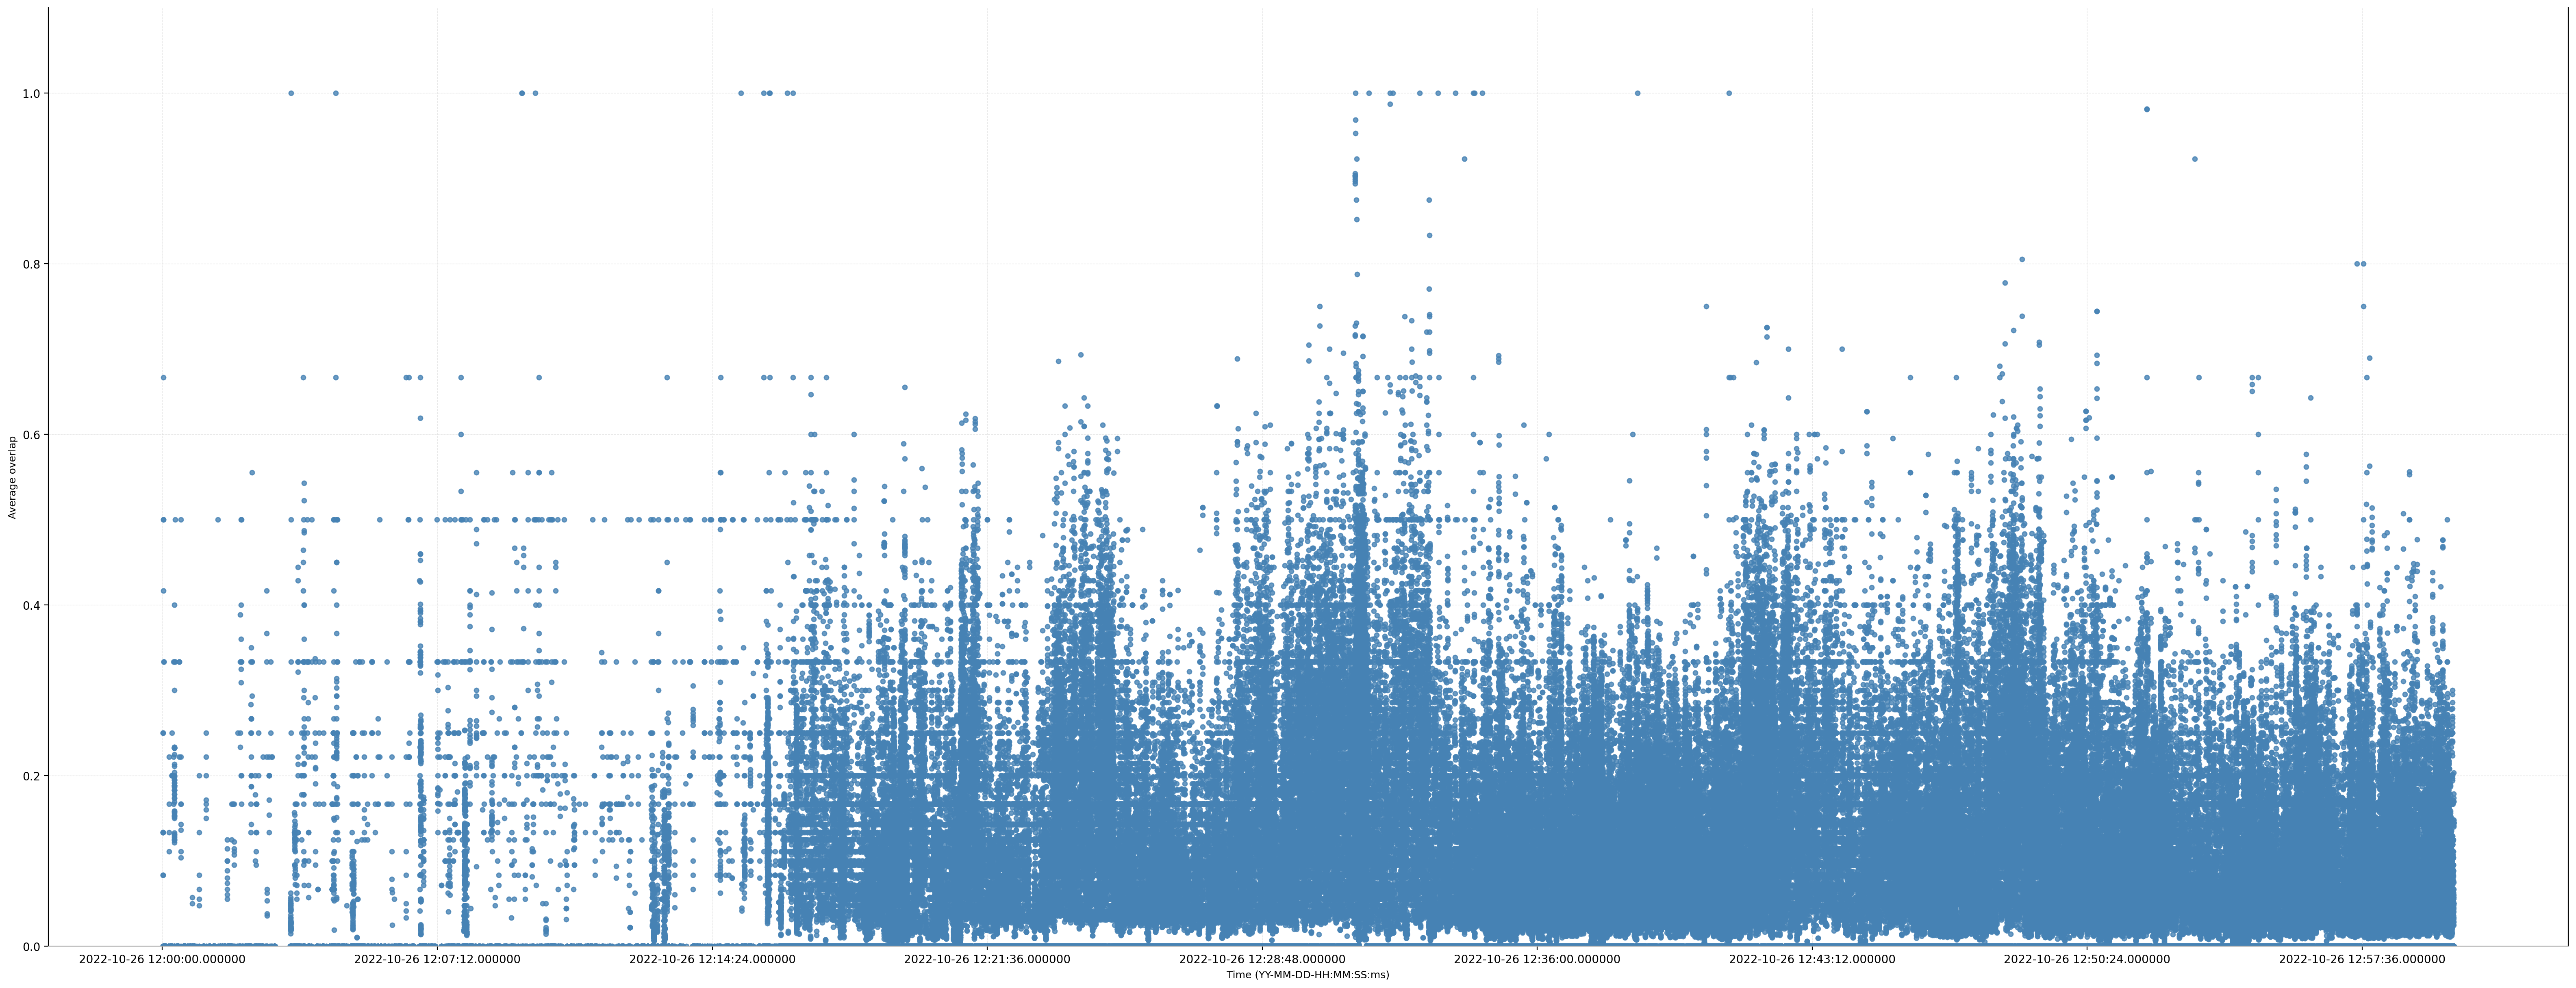
\includegraphics[width=1.45\textwidth, height=\textheight, keepaspectratio]{figures/plots/Scenario-1/G1-overlap-b0:f1:d8:50:92:c1-22-1652-351697-100ms.png}
  \caption[Overlap of Packet Success \& Failure with Rolling Time Average]{Scenario-1: Overlap values calculated using a rolling time window of 100ms. The x-axis represents the rolling timestamp values, while the y-axis shows the calculated overlap value. Further details on the calculation can be found in Section \ref{Overlap}.}
  \label{fig:overlap1}
\end{figure}
\FloatBarrier  
\end{landscape}

\begin{landscape}
\begin{figure}[hbt!]
  \centering
  \includegraphics[width=1.45\textwidth, height=\textheight, keepaspectratio]{figures/plots/Scenario-1/G1-MCS.vs.Time-heatprobabilitymap-b0:f1:d8:50:92:c1-22-1652-11652-100ms.png}
  \caption[Rate-Based Transmission Success Analysis with Rolling Time Averages]{Scenario-1: Success probability calculated using rolling time windows of 100ms. The x-axis represents the rolling timestamp values, while the y-axis shows the data rate followed by the specifications of each rate (Coding modulation - Bandwidth - Guard Interval - Number of spatial streams). The provided data represents a 15-minute timeline of Scenario-1.}
  \label{fig:Rolling-Success1}
\end{figure}
\FloatBarrier 
\end{landscape}


\begin{landscape}
\begin{figure}[hbt!]
  \centering
  \includegraphics[width=1.45\textwidth, height=\textheight, keepaspectratio]{figures/plots/Scenario-1/G1-MCS.vs.Time-coldprobabilitymap-b0:f1:d8:50:92:c1-22-1652-11652-100ms.png}
  \caption[Rate-Based Transmission Failure Analysis with Rolling Time Averages]{Scenario-1: Failed probability calculated using a rolling time windows of 100ms. The x-axis represents the rolling timestamp values, while the y-axis shows the data rate followed by the specifications of each rate (Coding modulation - Bandwidth - Guard Interval - Number of spatial streams). The provided data represents a 15-minute timeline of Scenario-1.}
  \label{fig:Rolling-Fail1}
\end{figure}
\FloatBarrier 
\end{landscape}




\subsection{Scenario-2 }
\label{sec:Analysis and Optimization:Performance Evaluation:Scenario2}
In this scenario, the channel exhibited a non-busy state, as presented in Figure~\ref{fig:populationmap-2}. The observation spanned an hour on October 26th, 2022, between 15:00 to 16:00 and focused on two stations utilizing the same radio~(phy~1). The full observation over network traffic shows the presence of station "b0:f1:d8:50:92:c1"\cite{SNCX_internal_note} which is the target device for all the plots in scenario-2.

The corresponding signal strength value plot in Figure~\ref{fig:rxs-2} illustrates consistently stable transmission power, surpassing 60~dBm, which can be an indicator for the station to have close stable distance to AP during this time, as well as the proof for station to be environmentally static and stable.

The number of attempted packets, as evidenced by Figure~\ref{fig:Attempt2}, is lower compared to Scenario-1~\ref{sec:Analysis and Optimization:Performance Evaluation:Scenario1}, indicating that only 7 rates were traversed in general with lower number of transmission (the colorbar gives the exact number of transmission for each tried rates), it is valuable to additionally mention that, the low network traffic is also observable in \ref{sec:data_set}, which demonstrates our observation as to why Minstrel-HT is not searching for different rates and why it is not exploring the entire rate space for an alternative rates. Minstrel-HT is keeping the rates which give the high performance outcome, due to low stream of traffic, the algorithm is not probing(sampling) that many jump rates\ref{sec:intro:minstrelht:probing}, let's keep in mind the period of updating sampling queue is 50~Hz (20~milliseconds), and low traffic prevents the chance that so many rates from queue have chance to be probed. considering all the evidences, the low exploration of rates is reasonable in this context.

In the following, figure~\ref{fig:Success-count2}, the number of acknowledged packet per each rate is observable. The rate within group~9 demonstrated remarkably high successful acknowledged transmissions along with high success probabilities, as depicted in Figure~\ref{fig:Success-probability2}. By evaluating success probability ~\ref{fig:Success-probability2} and success packet count ~\ref{fig:Success-count2} it is apparent in stable channel scenario, faster Modulations with more spatial streams and 40 MHz bandwidth have higher chance to be chosen by Minstrel-HT. The successful probability for rates within group~9 is higher than group~d, engaging to one to one comparison of rates group;

Group 9: Hight troughput- 40 MHz Badwidth - Long Guard Interval -2 spatial stream\\
Group d: Hight troughput- 40 MHz Badwidth - short Guard Interval -2 spatial stream\\
In this scenario,a longer guard interval exhibits a higher higher probability of success. Furthermore, Figure~\ref{fig:Success-p-vs-airtime2} highlights that the fastest rates, characterized by lower airtimes, achieve exceptionally high success probabilities. In detail, the plot of successful rates selected by algorithm over time in~\ref{fig:Rolling-Success2} shows the preference of rate selection by Minstrel-HT. As mentioned earlier, a stable channel is observable in this plot, where the probability of selected rates remains generally stable over time and exceeds 80~percent success rate. This is in contrast to scenario-1 (Section~\ref{sec:Analysis and Optimization:Performance Evaluation:Scenario1}), as shown in Figure~\ref{fig:Rolling-Success1}, where such a stable rate selection is not evident due to channel instability and other discussed aspects~\ref{sec:Analysis and Optimization:Performance Evaluation:Scenario1}.

The plots~\ref{fig:Fail-count2} and~\ref{fig:Fail-probability2} are complement sets to the corresponding successful values as it's observable. The most successful rates scored lowest failure values.

Moving to overlap plot, due to the reduced number of packet transmissions, the overlap depicted in Figure~\ref{fig:overlap2} demonstrates higher values. This occurrence can be correlated to a higher likelihood of encountering both successful and failed attempts within the same rate. Therefore, for further investigations on the overlap between successful and failed rates, it is crucial to consider and evaluate the quantity of packet transmissions as a key factor and as mentioned in section-2, this area can be in the scope of future research to find the best time interval for statistical updates for rates slection in Minstrel-HT,considering the channel traffic.



\begin{landscape}
\begin{figure}[hbt!]
  \centering
  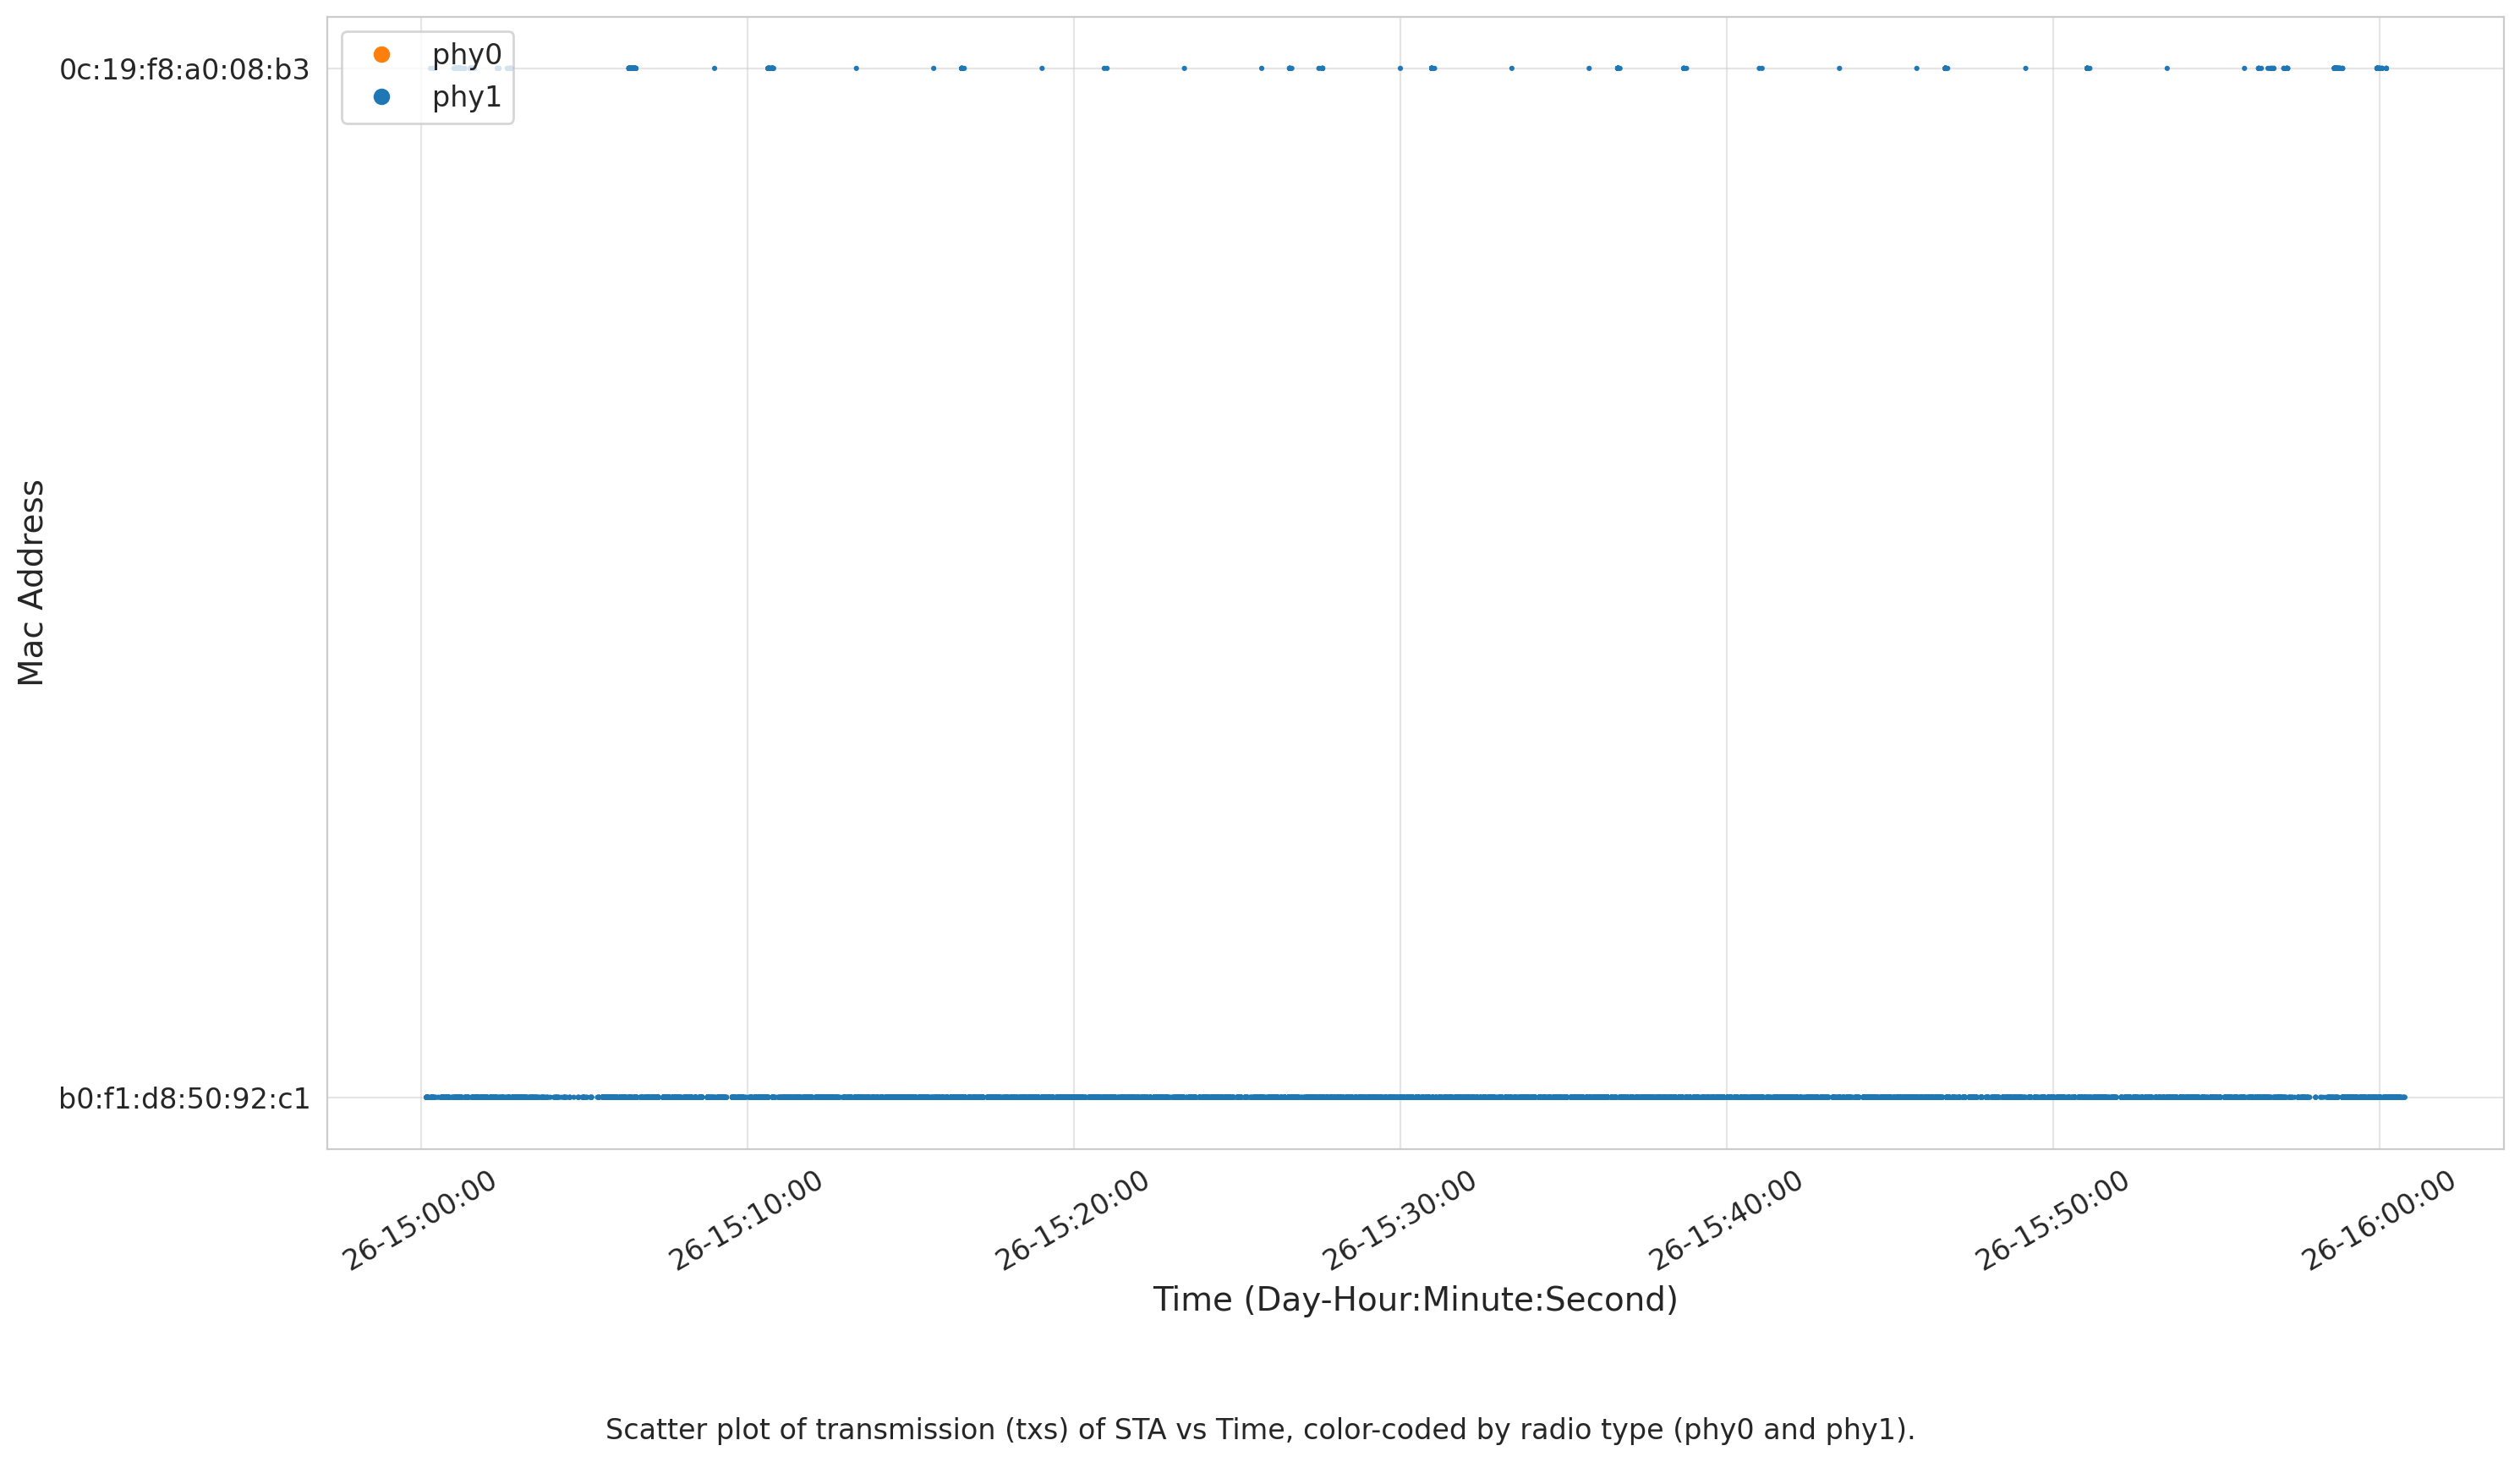
\includegraphics[width=1.45\textwidth, height=\textheight, keepaspectratio]{figures/plots/Scenario-2/G2-22.png}
  \caption[Transmission of stations Over Time]{Scenario-2: Transmission of Stations Over Time: All active stations in the channel are represented by their MAC addresses. The orange color indicates transmission via radio Phy0, while the blue color represents transmission via Phy1.}
  \label{fig:populationmap-2}
\end{figure}
\FloatBarrier 
\end{landscape}

\begin{landscape}
\begin{figure}[hbt!]
  \centering
  \includegraphics[width=1.45\textwidth, height=\textheight, keepaspectratio]{figures/plots/Scenario-2/G2-RSSI-b0:f1:d8:50:92:c1.png}
  \caption[Temporal Analysis of Signal Strength]{Scenario-2: Temporal Analysis of Signal Strength: Signal strength values in dBm over a course of time. Lower values indicate weaker signal strength.}
  \label{fig:rxs-2}
\end{figure}
\FloatBarrier 
\end{landscape}


\begin{figure}[hbt!]
  \centering
  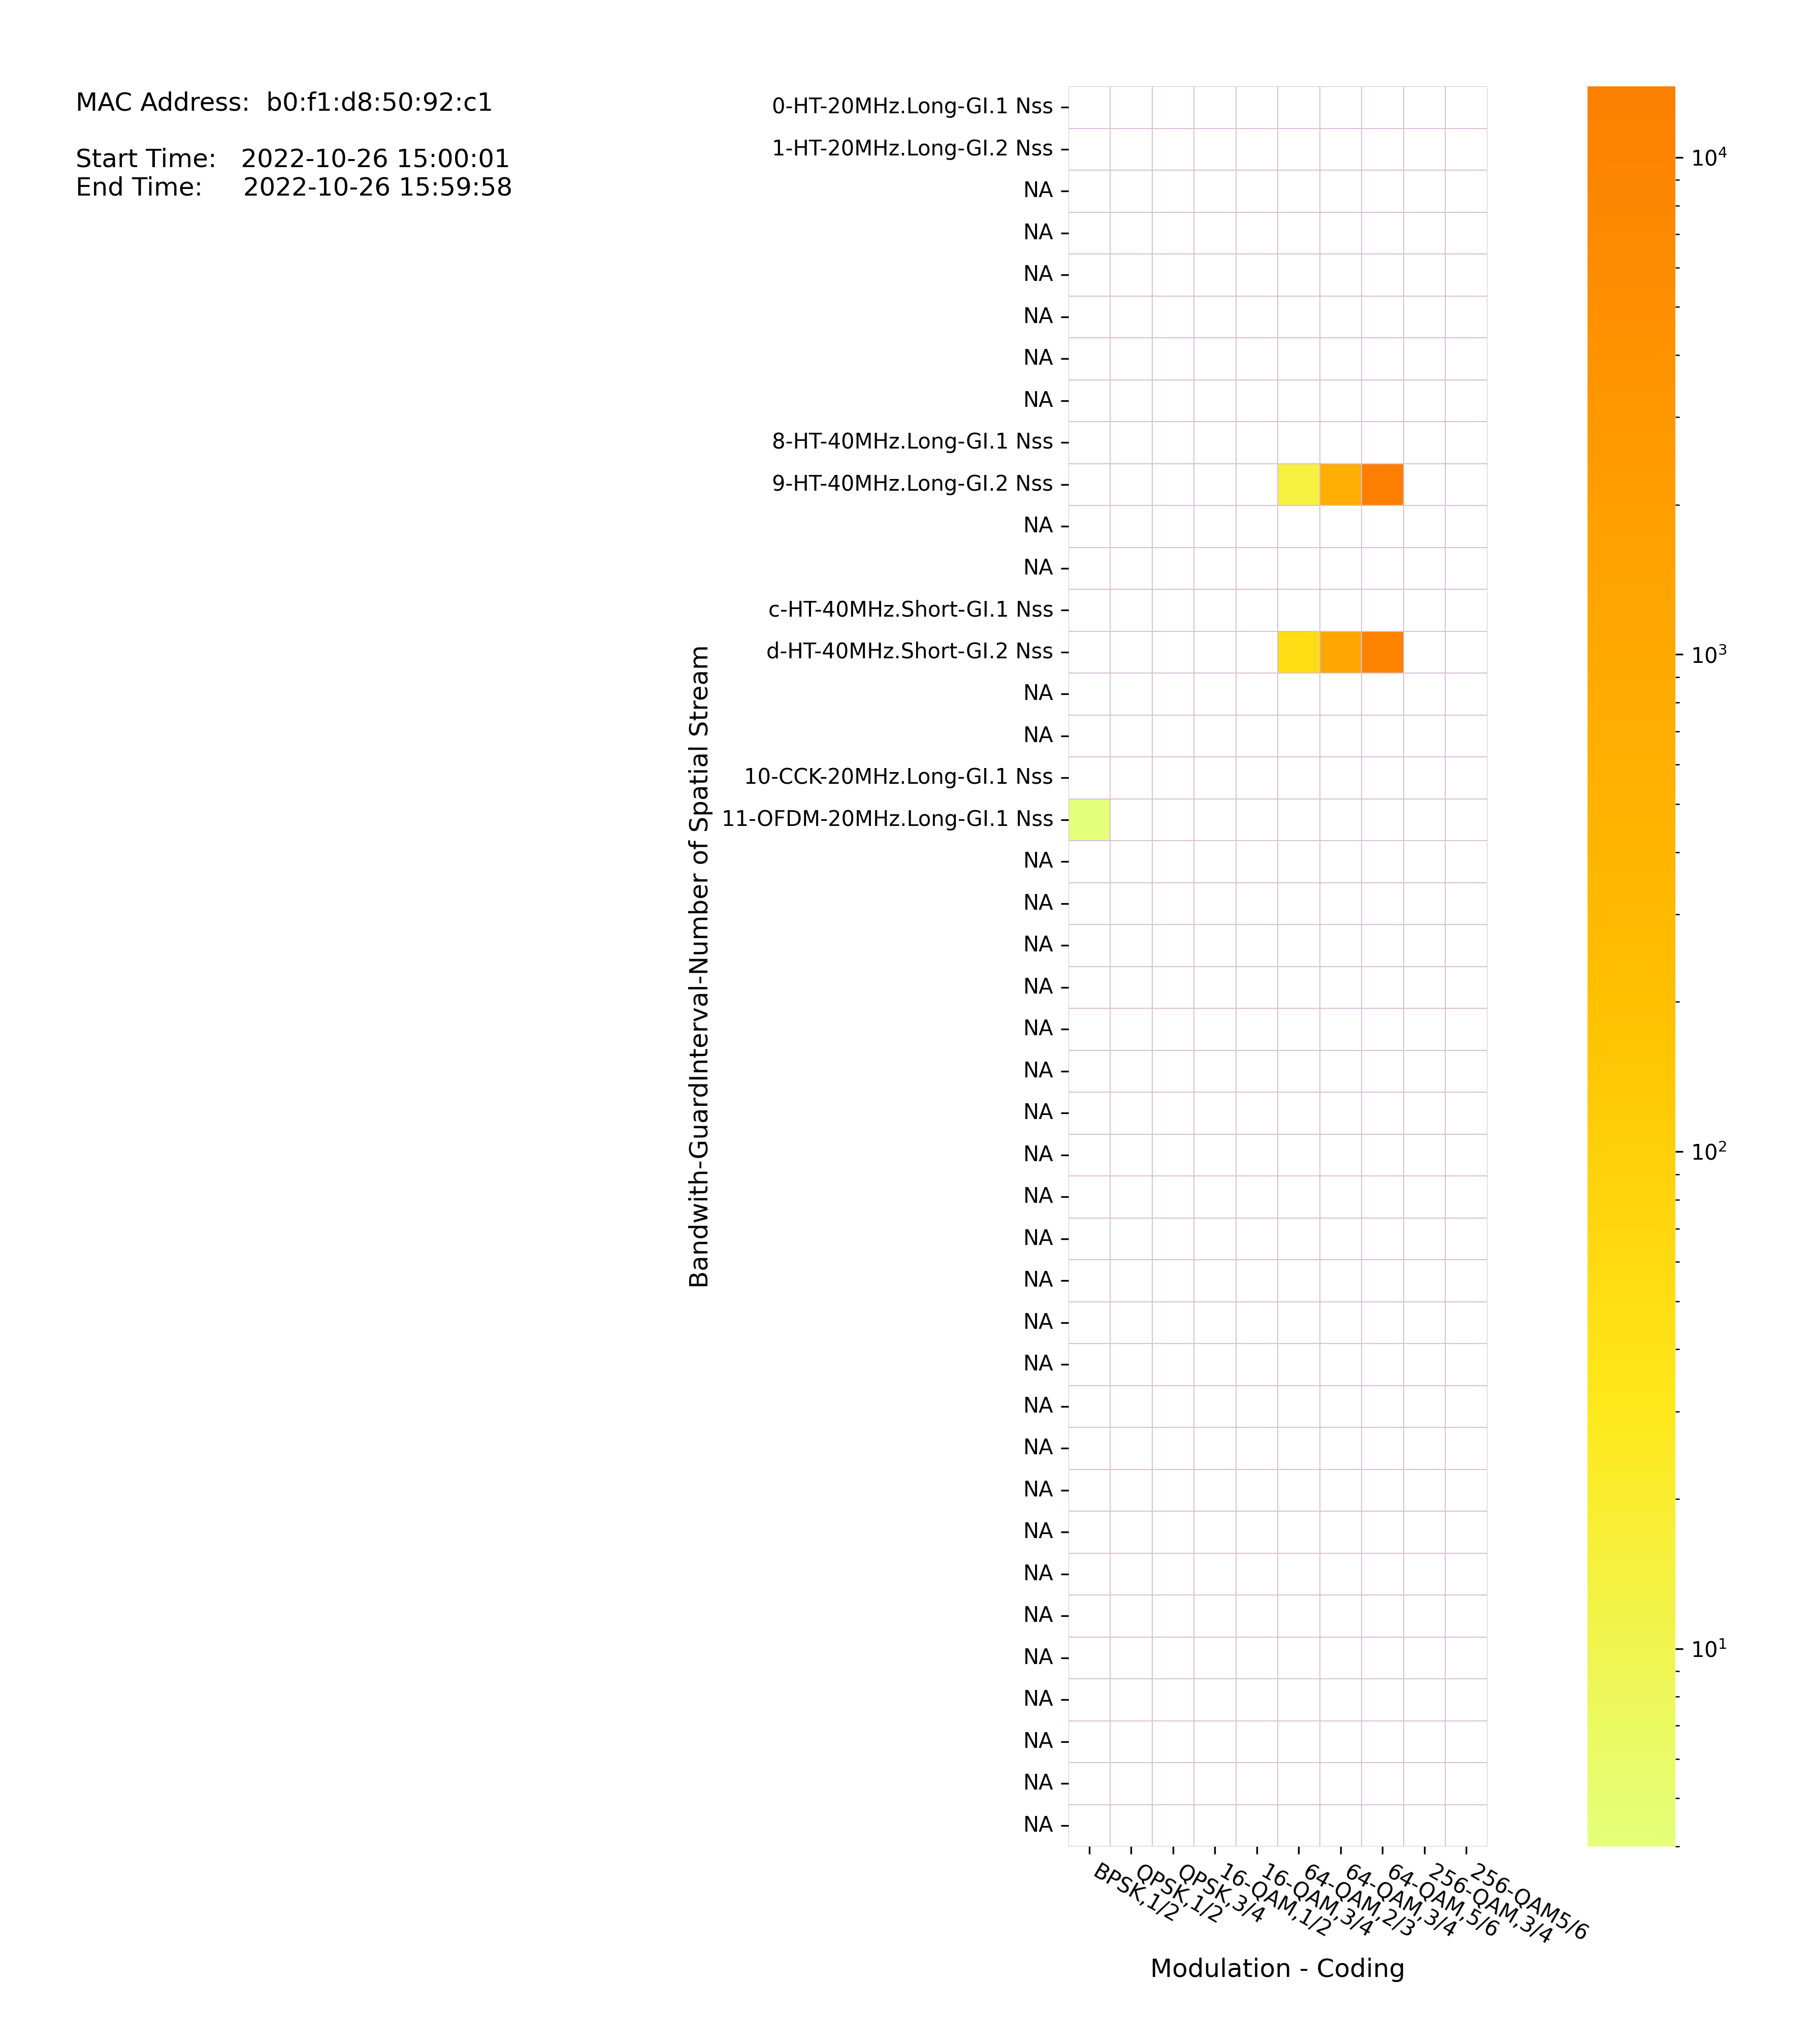
\includegraphics[width=\textwidth]{figures/plots/Scenario-2/G2-attemptmap-b0:f1:d8:50:92:c1-22-431070-450182.png}
  \caption[Transmission Status]{Scenario-2: Transmitted rates per rates group index over Modulation and Coding. The colorbar represents the number of transmitted packets (ACK and Non-Ack). The start and end times of observation, as well as the MAC address of the station, are indicated in the plot.}
  \label{fig:Attempt2}
\end{figure}
\FloatBarrier 


\begin{figure}[hbt!]
  \centering
  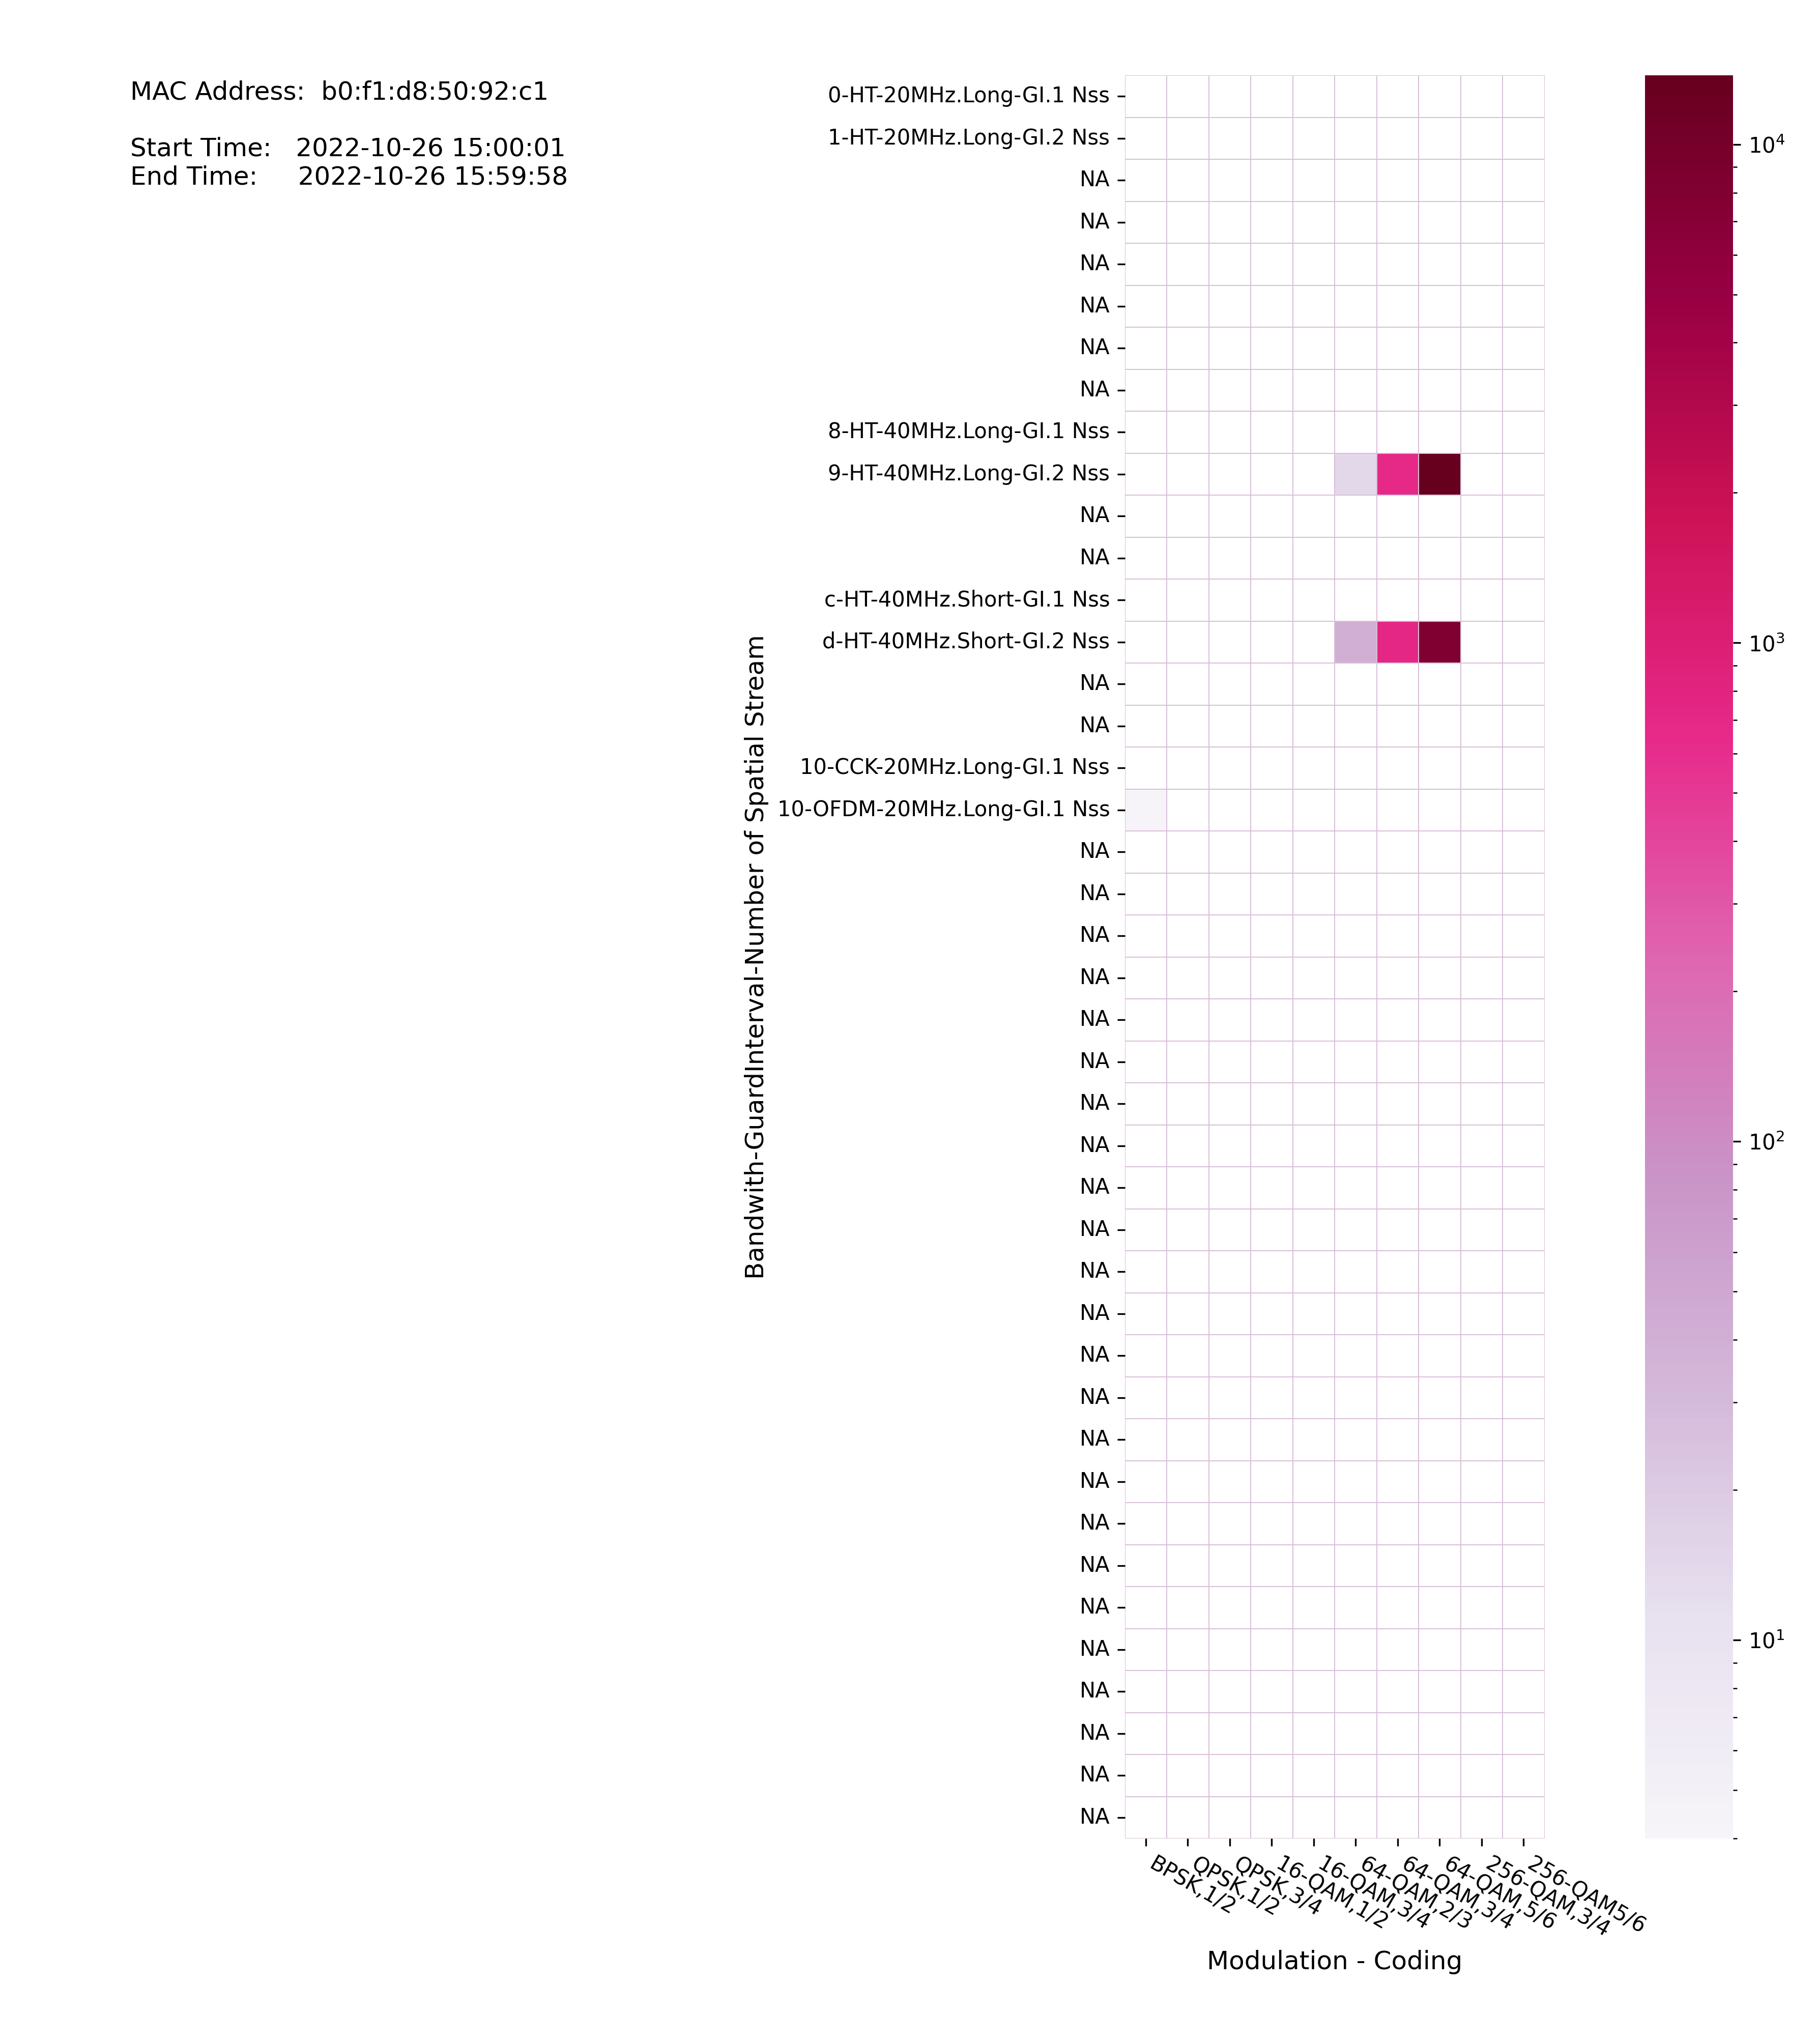
\includegraphics[width=\textwidth]{figures/plots/Scenario-2/G2-heatmap-b0:f1:d8:50:92:c1-22-431070-450182.png}
  \caption[Rate-Based Packet Success Analysis]{Scenario-2: Successfully transmitted rates per rates group index over Modulation and Coding. The colorbar represents the number of successfully transmitted packets (ACK). The start and end times of observation, as well as the MAC address of the station, are indicated in the plot.}
  \label{fig:Success-count2}
\end{figure}
\FloatBarrier 


\begin{figure}[hbt!]
  \centering
  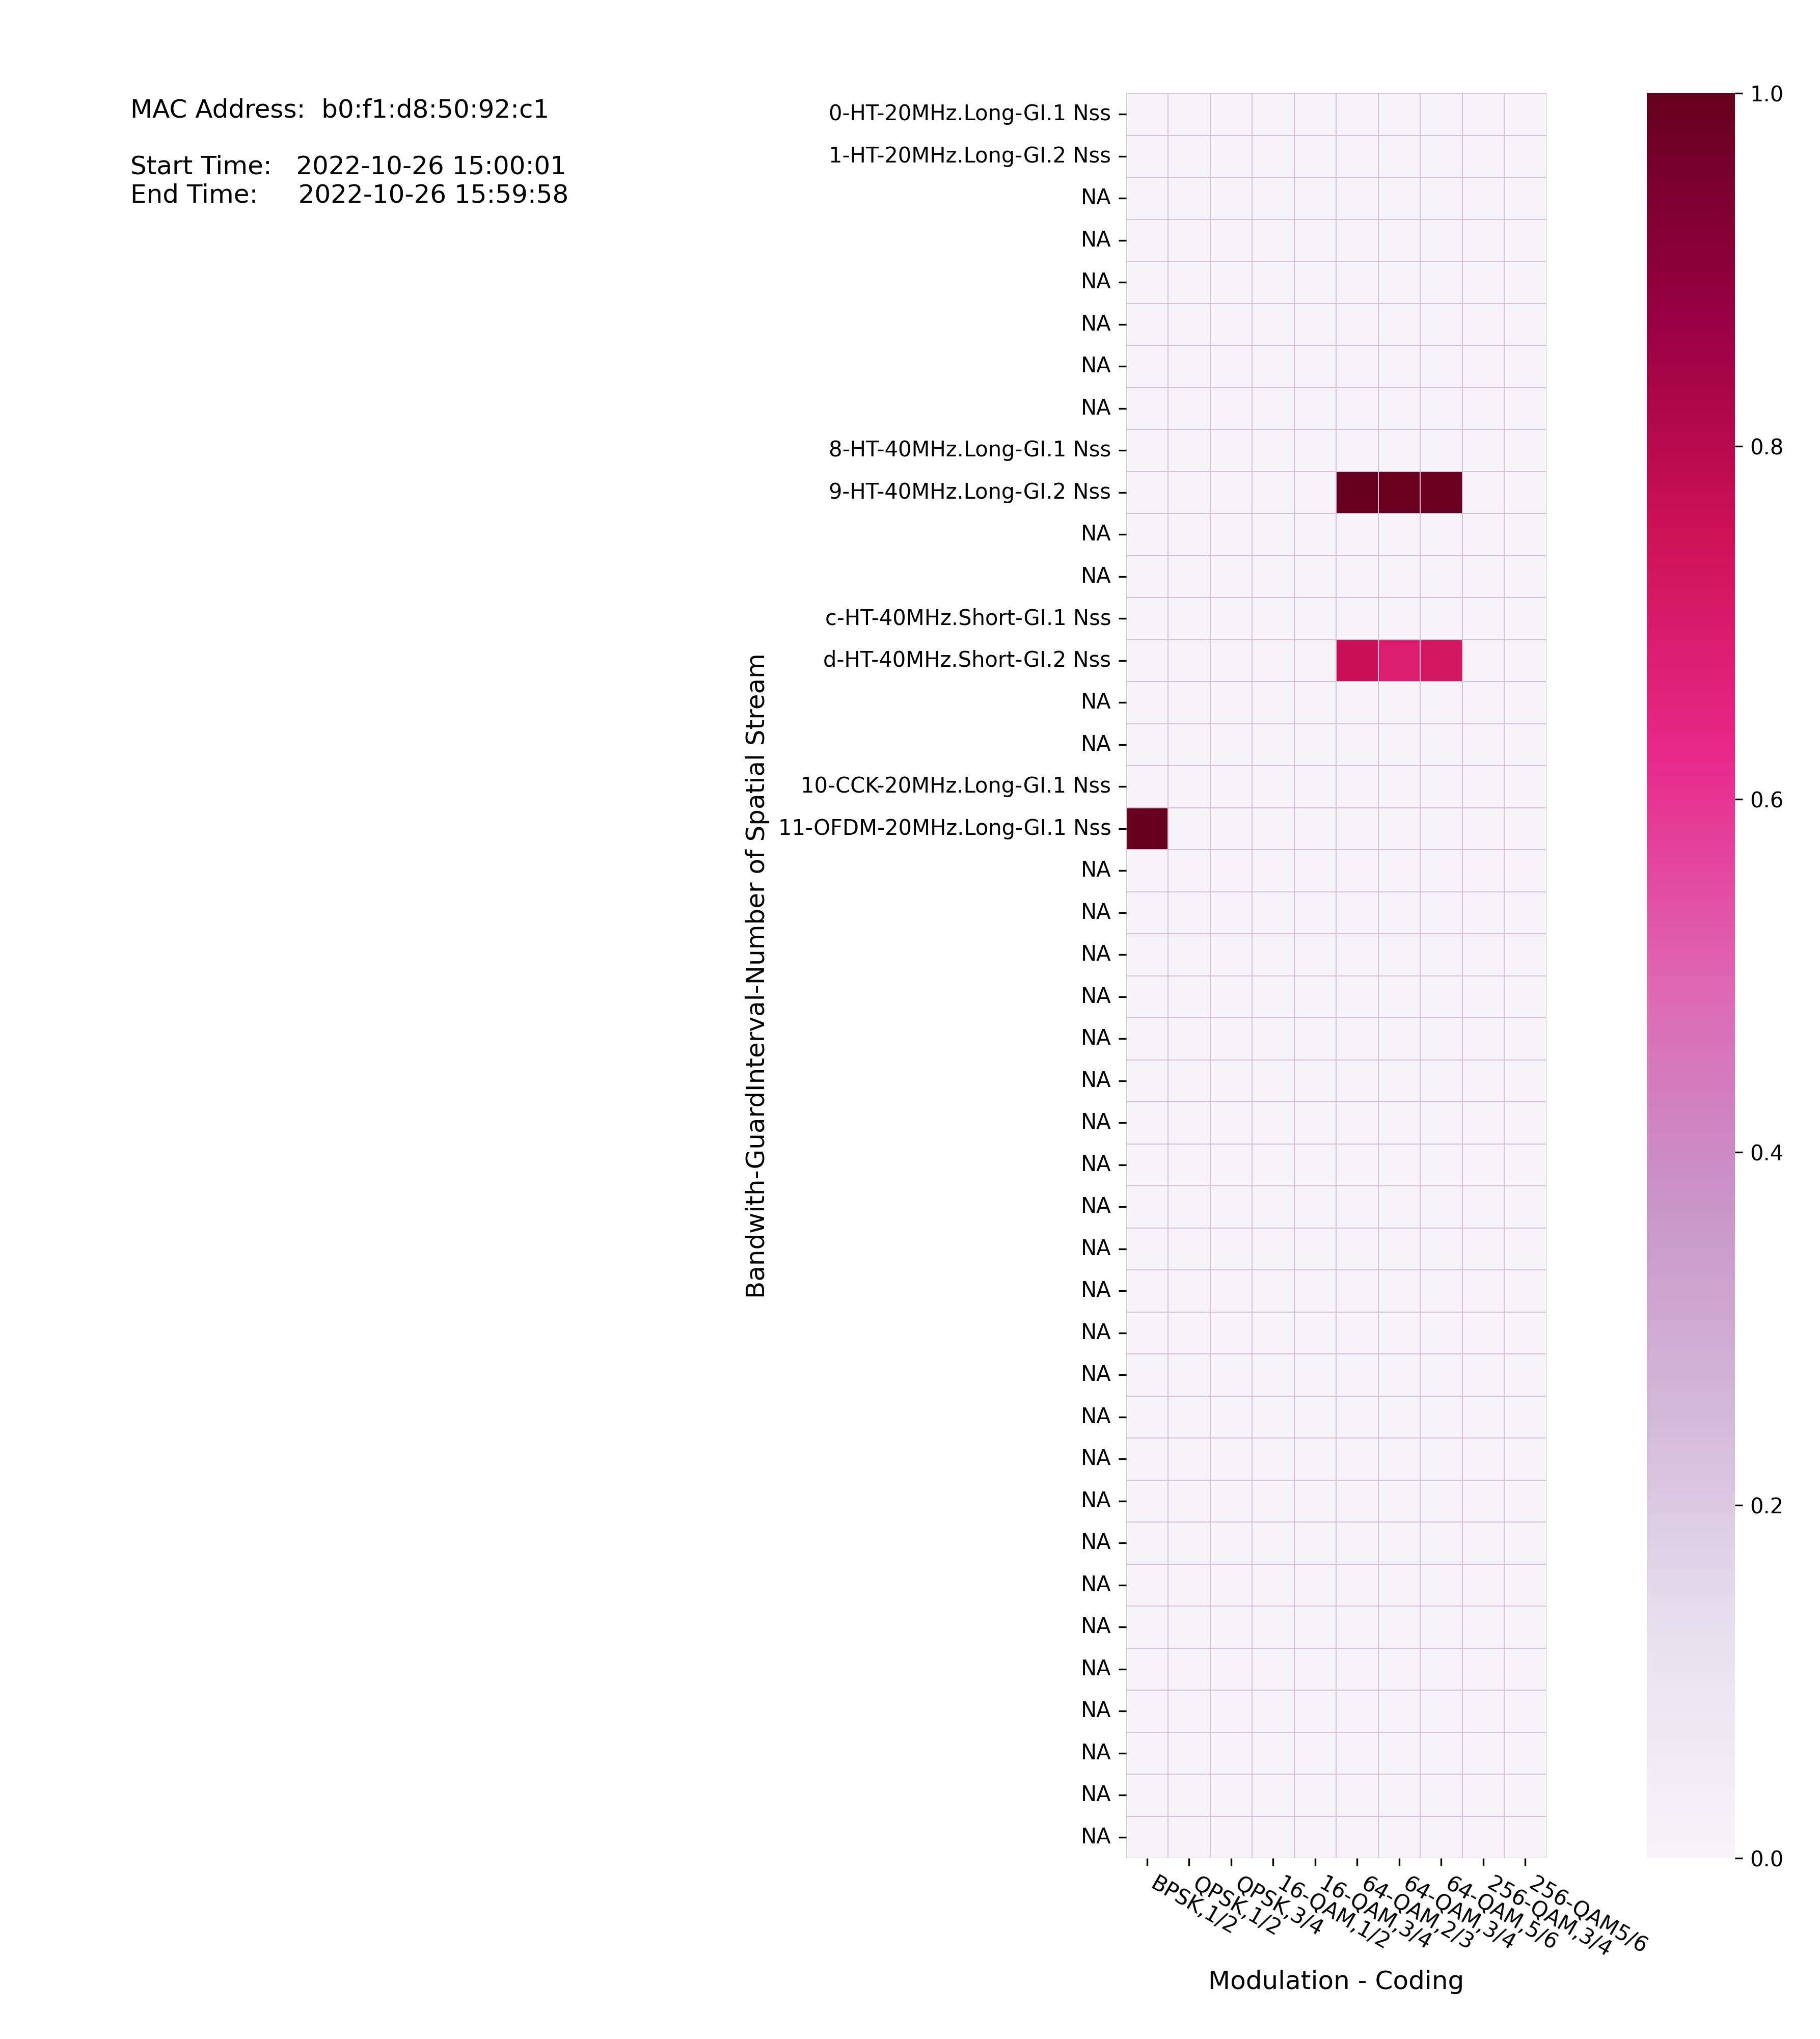
\includegraphics[width=\textwidth]{figures/plots/Scenario-2/G2-heatmap-p-b0:f1:d8:50:92:c1-22-431070-450182.png}
  \caption[Probability of Success for Rate-Based Transmission]{Scenario-2: Probability of successfully transmitted rates per rates group index over Modulation and Coding. The colorbar represents the probability scaled from 0 to 1.}
  \label{fig:Success-probability2}
\end{figure}
\FloatBarrier 

\begin{landscape}
\begin{figure}[hbt!]
  \centering
  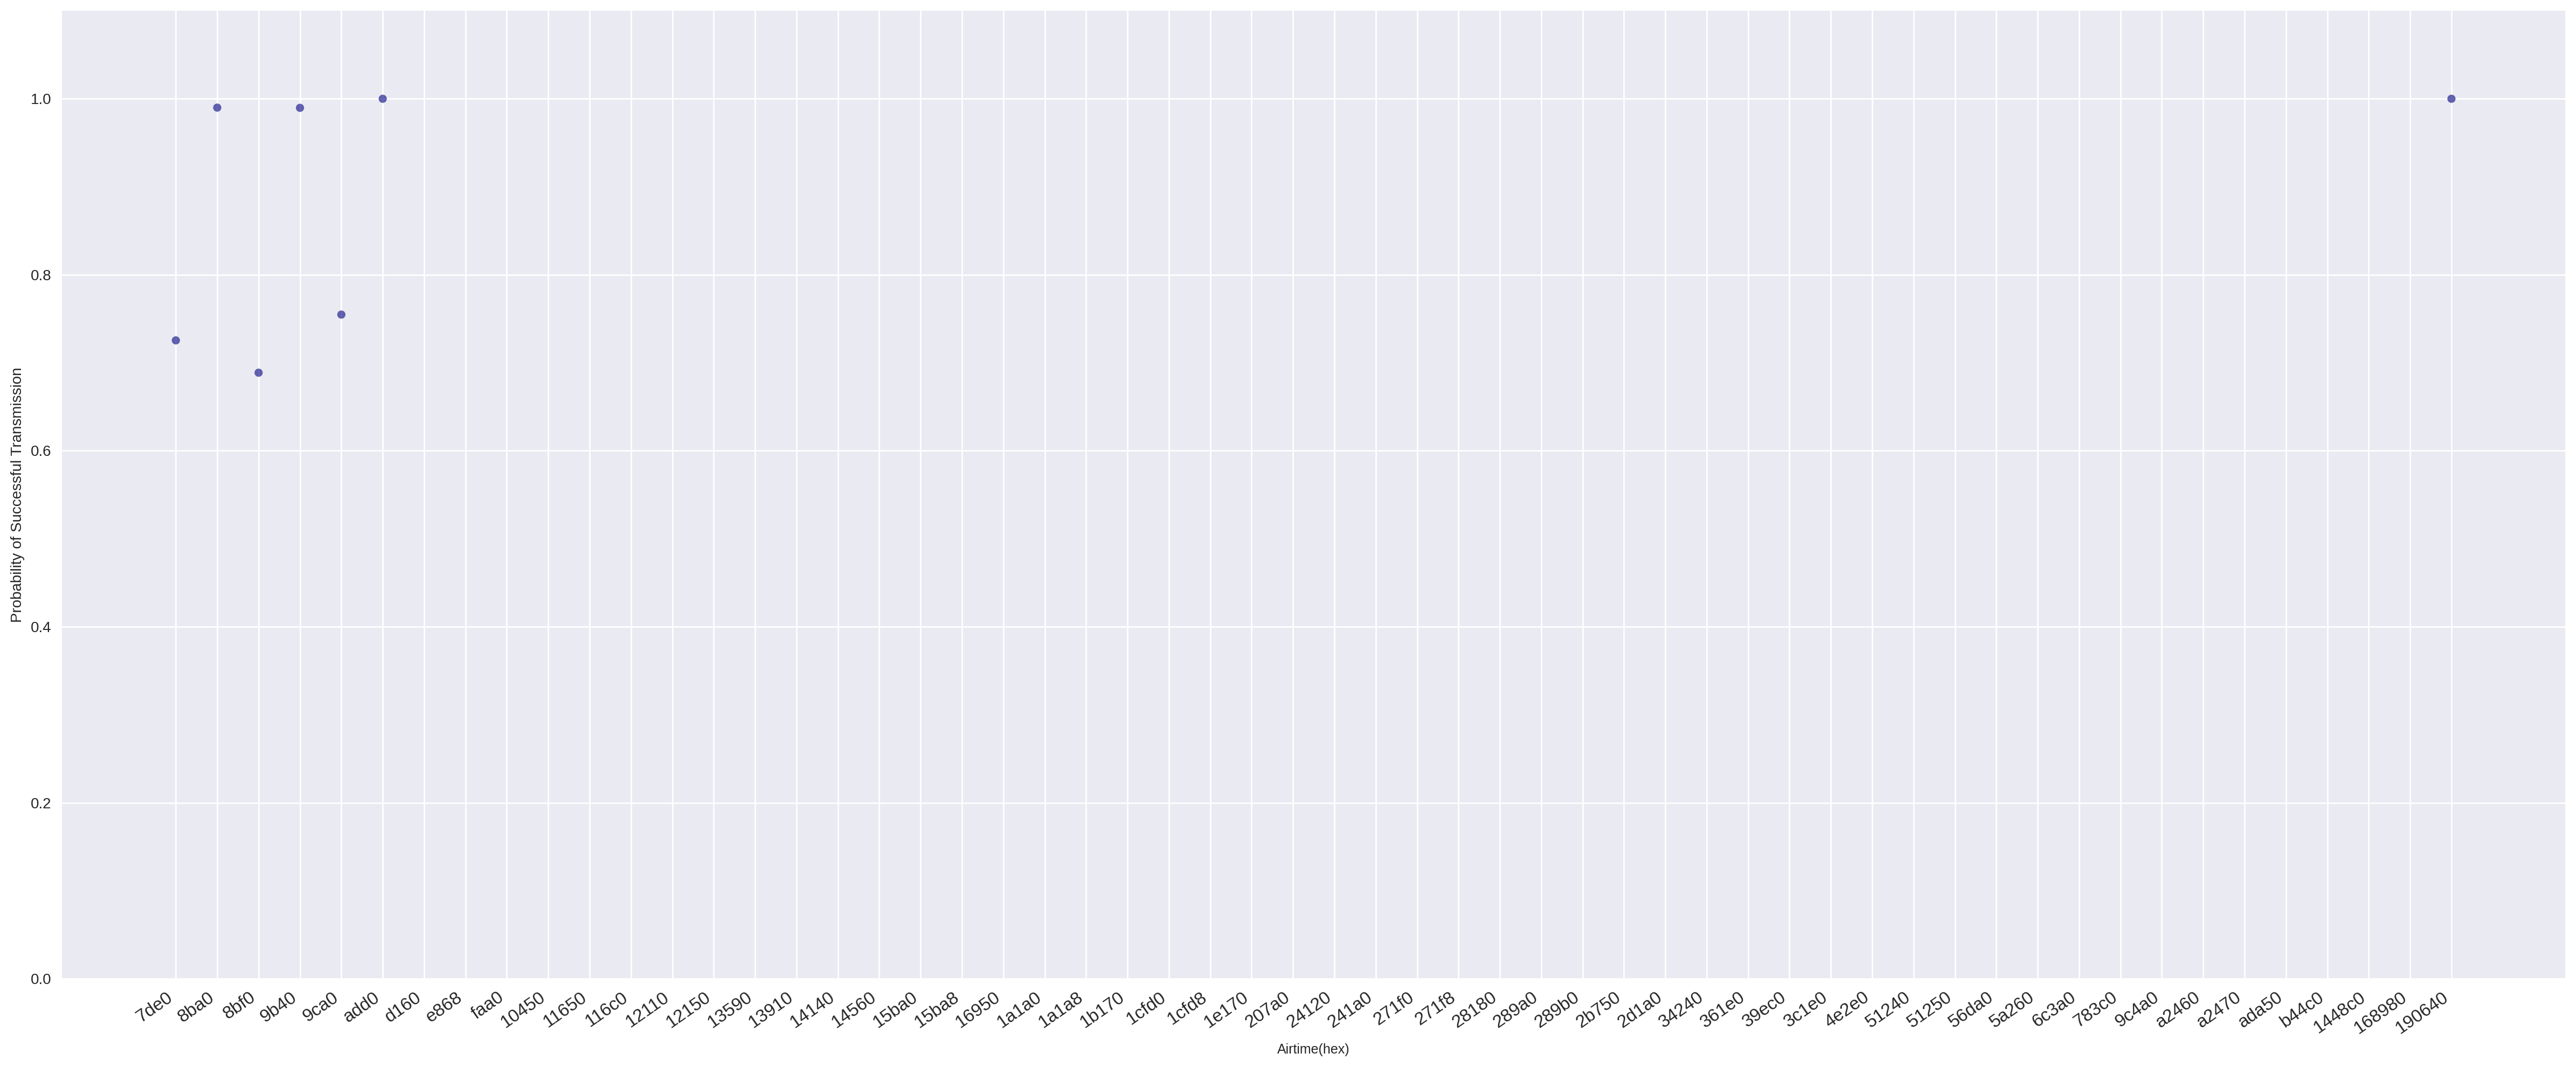
\includegraphics[width=1.45\textwidth, height=\textheight, keepaspectratio]{figures/plots/Scenario-2/G2-probability vs airtime-b0:f1:d8:50:92:c1-22-431070-450182.png}
  \caption[Airtime-Based Success Probability for Rate-Based Transmission]{Scenario-2: Airtime values in nanoseconds (hex notation) on the x-axis, and the probability of success on the y-axis.}
  \label{fig:Success-p-vs-airtime2}
\end{figure}
\FloatBarrier 
\end{landscape}

\begin{landscape}
\begin{figure}[hbt!]
  \centering
  \includegraphics[width=1.45\textwidth, height=\textheight, keepaspectratio]{figures/plots/Scenario-2/G2-MCS.vs.Time-heatprobabilitymap-b0:f1:d8:50:92:c1-22-431070-450182-100ms.png}
  \caption[Rate-Based Transmission Success Analysis with Rolling Time Averages]{Scenario-2: Success probability calculated using rolling time windows of 100ms. The x-axis represents the rolling timestamp values, while the y-axis shows the data rate followed by the specifications of each rate (Coding modulation - Bandwidth - Guard Interval - Number of spatial streams). The provided data represents a 15-minute timeline of Scenario-1.}
  \label{fig:Rolling-Success2}
\end{figure}
\FloatBarrier 
\end{landscape}

\begin{figure}[hbt!]
  \centering
  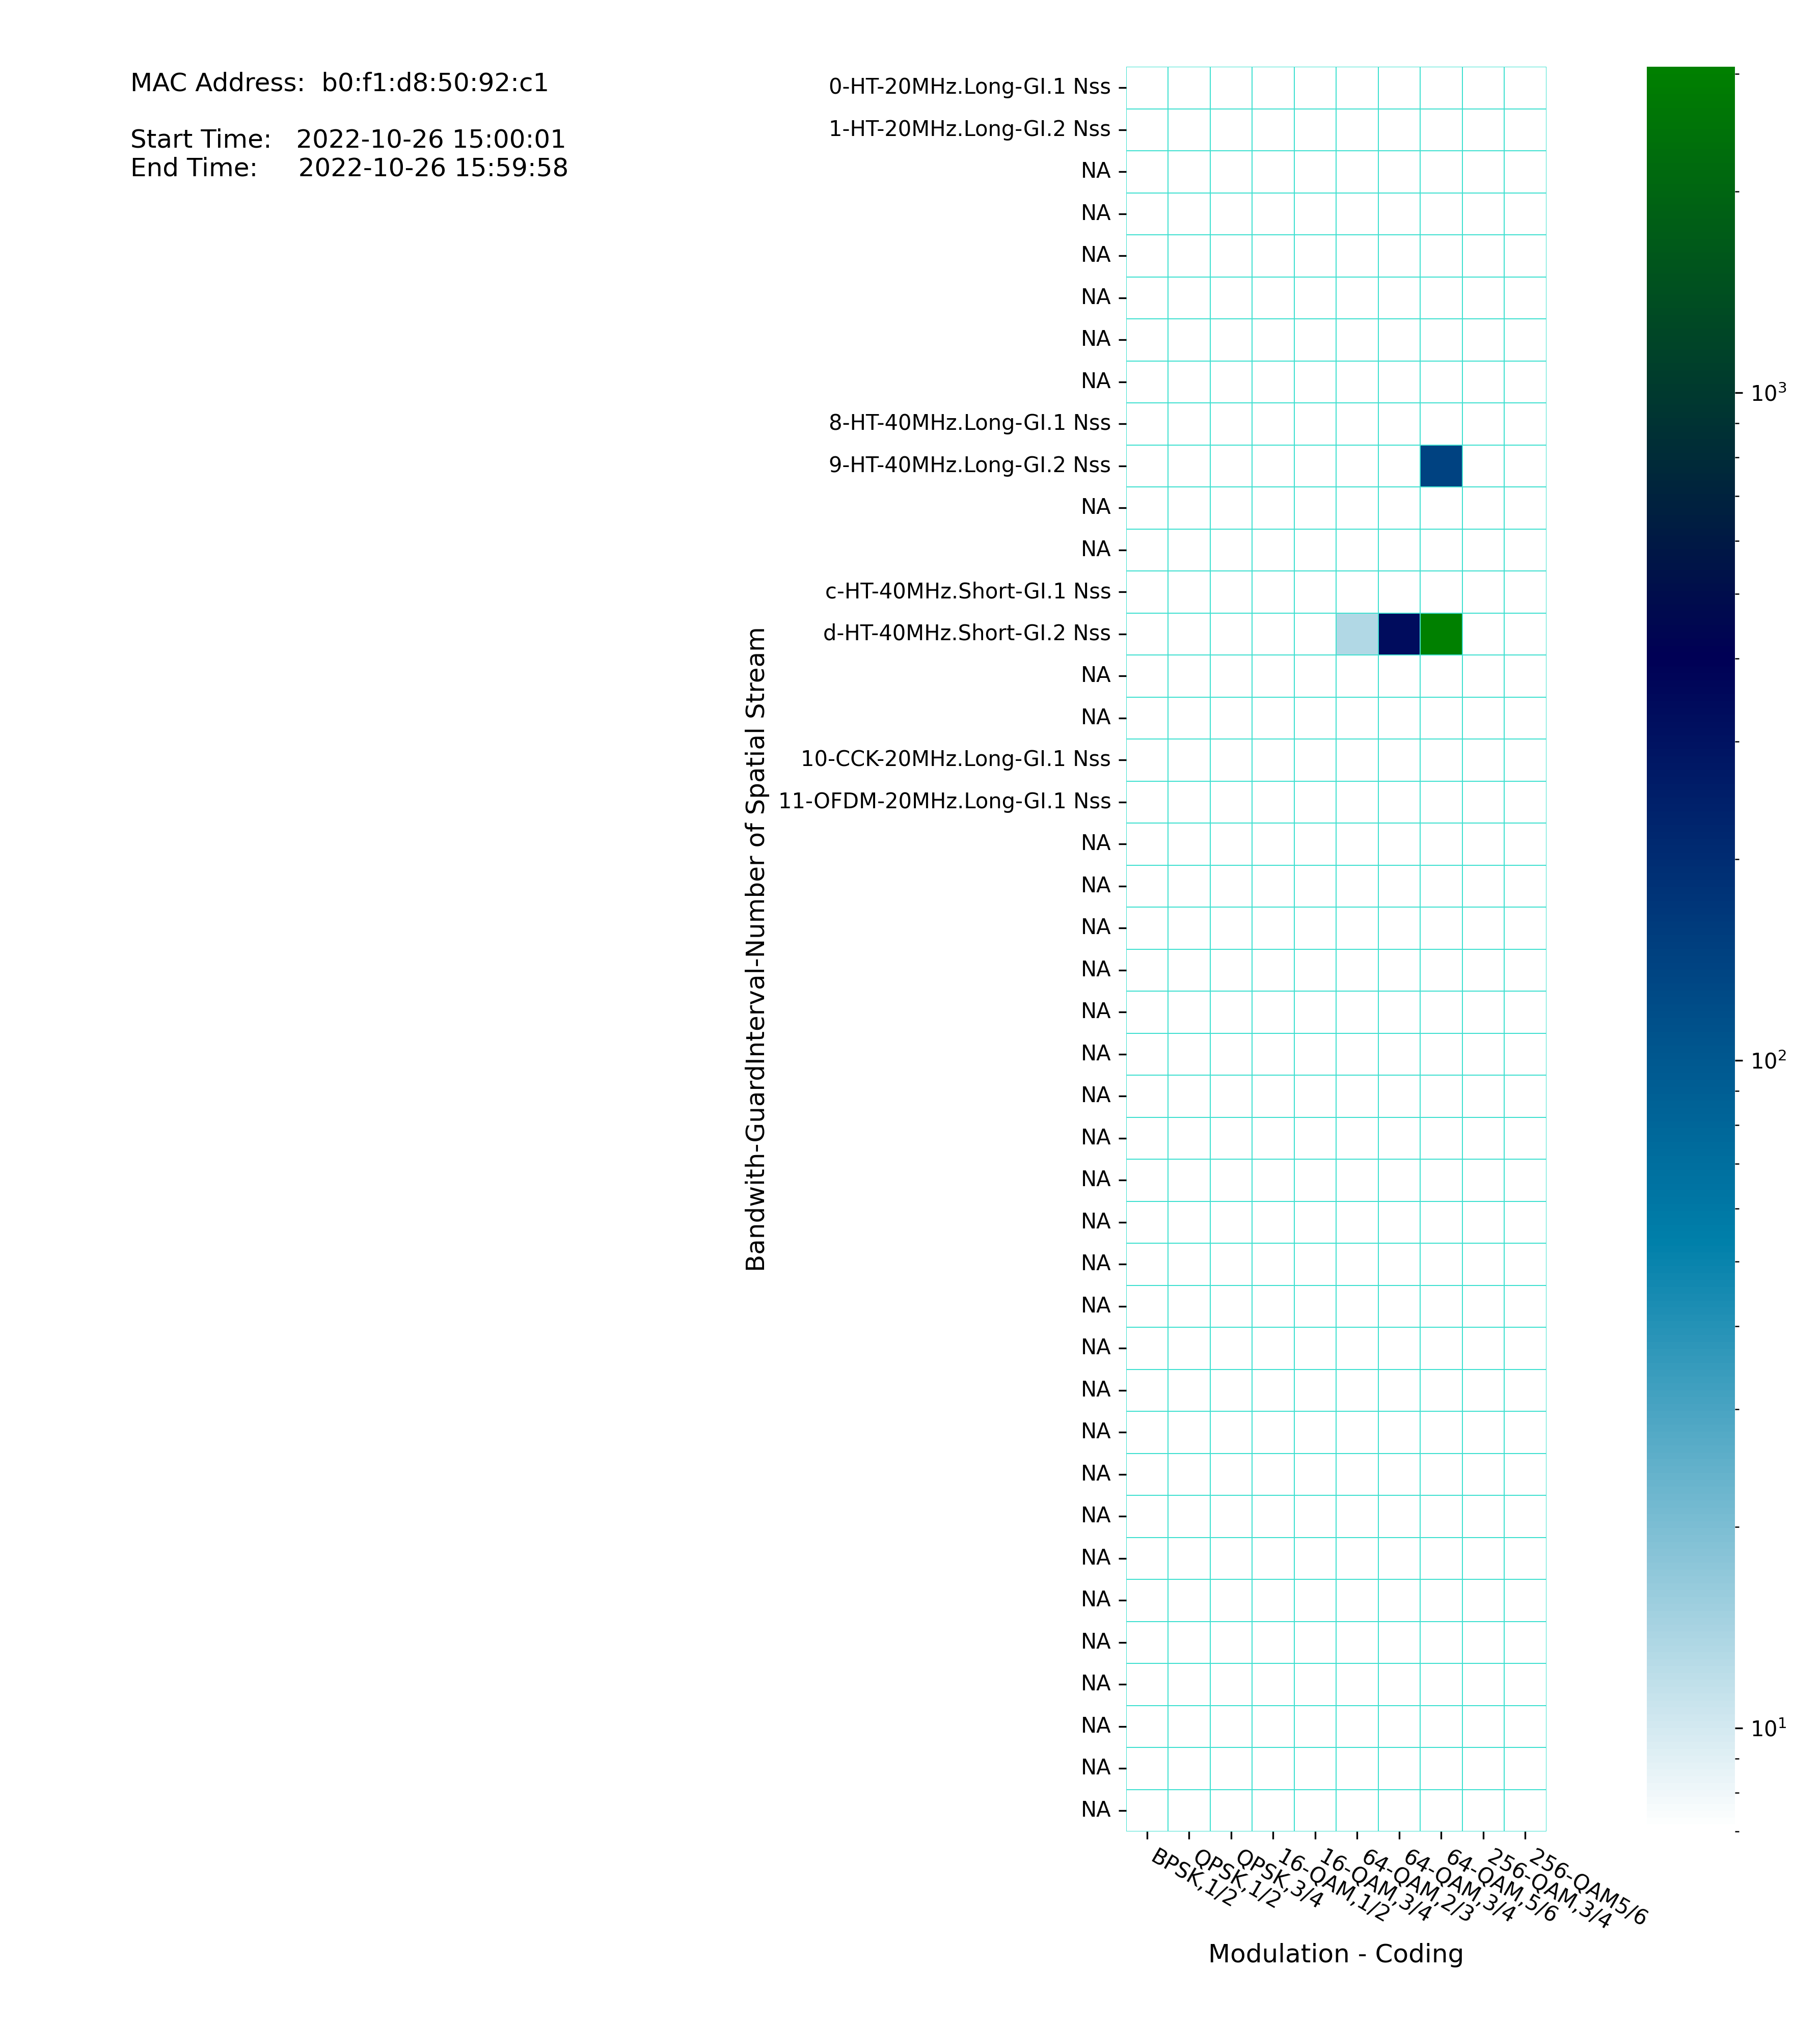
\includegraphics[width=\textwidth]{figures/plots/Scenario-2/G2-coldmap-b0:f1:d8:50:92:c1-22-431070-450182.png}
  \caption[Rate-Based Packet Failure Analysis]{Scenario-2: Failed transmitted rates per rates group index over Modulation and Coding. The colorbar represents the number of failed transmitted packets (Non-ACK). The start and end times of observation, as well as the MAC address of the station, are indicated in the plot.}
  \label{fig:Fail-count2}
\end{figure}
\FloatBarrier 

\begin{figure}[hbt!]
  \centering
  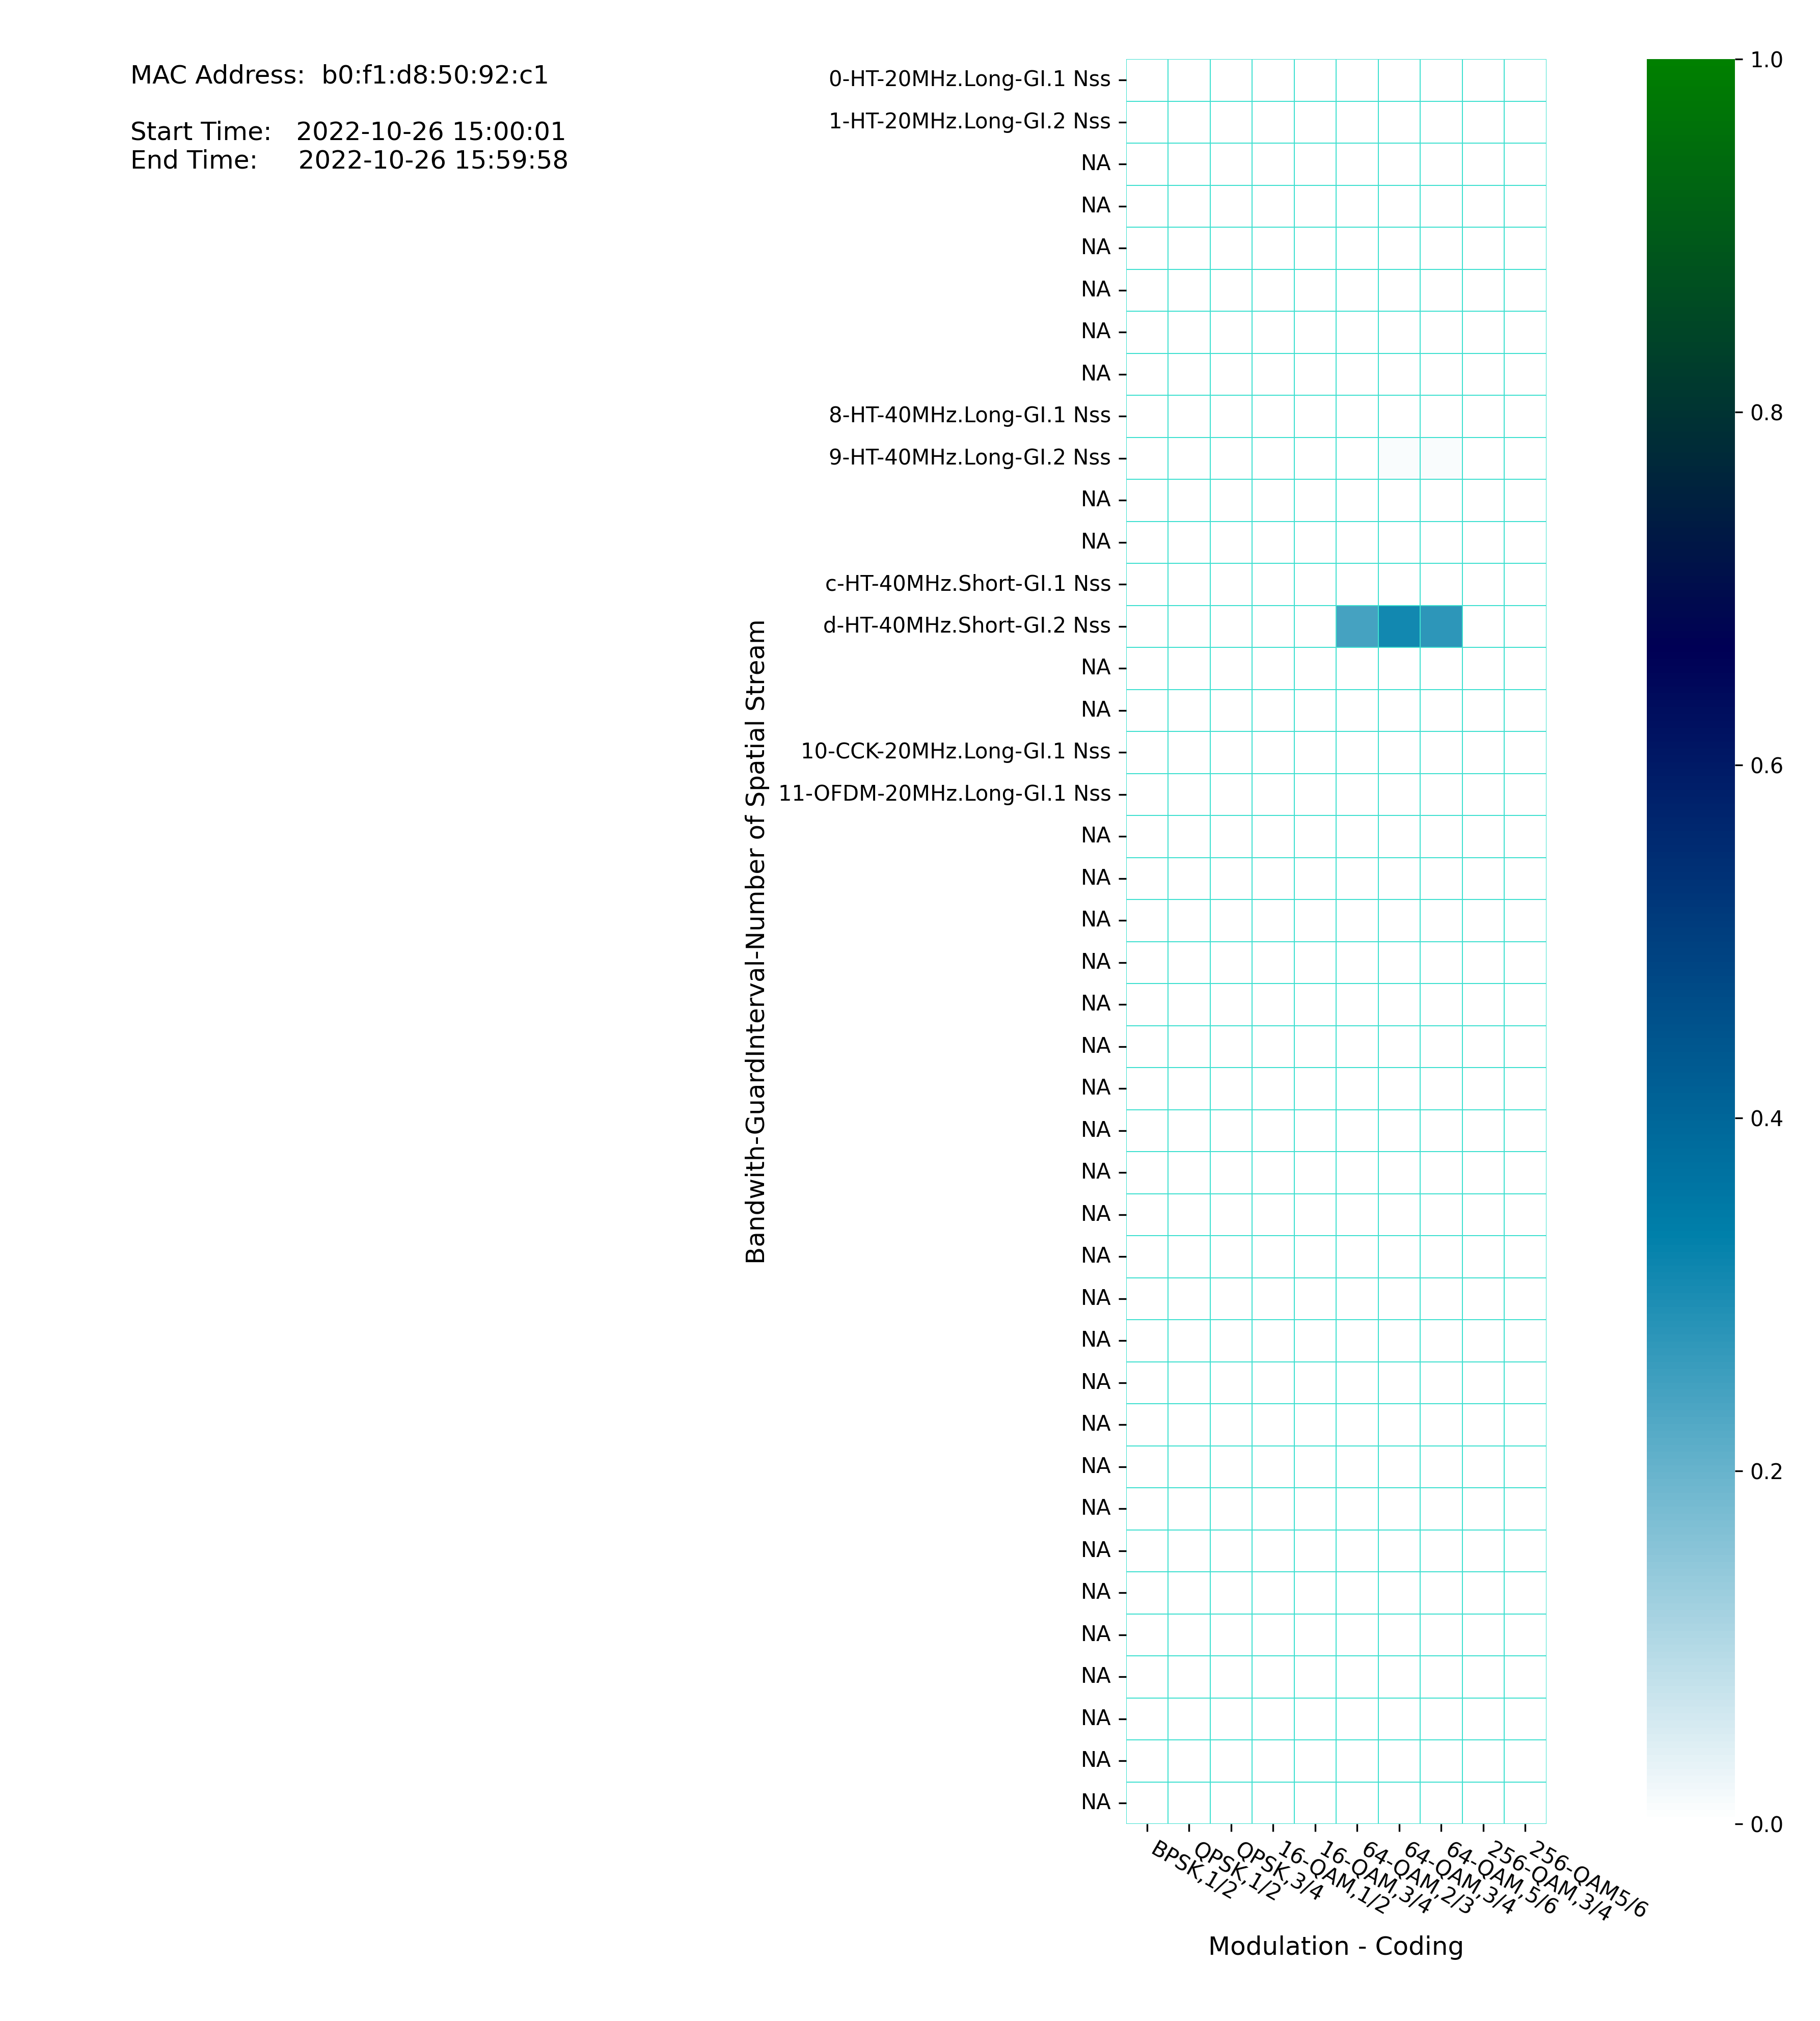
\includegraphics[width=\textwidth]{figures/plots/Scenario-2/G2-coldmap-p-b0:f1:d8:50:92:c1-22-431070-450182.png}
  \caption[Rate-Based Transmission Failure Analysis]{Scenario-2: Probability of failed transmitted rates per rates group index over Modulation and Coding. The colorbar represents the probability scaled from 0 to 1.}
  \label{fig:Fail-probability2}
\end{figure}
\FloatBarrier 

\begin{landscape}
\begin{figure}[hbt!]
  \centering
  \includegraphics[width=1.45\textwidth, height=\textheight, keepaspectratio]{figures/plots/Scenario-2/G2-MCS.vs.Time-coldprobabilitymap-b0:f1:d8:50:92:c1-22-431070-450182-100ms.png}  
  \caption[Rate-Based Transmission Failure Analysis with Rolling Time Averages]{Scenario-2: Failed probability calculated using a rolling time windows of 100ms. The x-axis represents the rolling timestamp values, while the y-axis shows the data rate followed by the specifications of each rate (Coding modulation - Bandwidth - Guard Interval - Number of spatial streams). The provided data represents a 15-minute timeline of Scenario-1.}
  \label{fig:Rolling-Fail2}
\end{figure}
\FloatBarrier 
\end{landscape}


\begin{landscape}
\begin{figure}[hbt!]
  \raggedright
  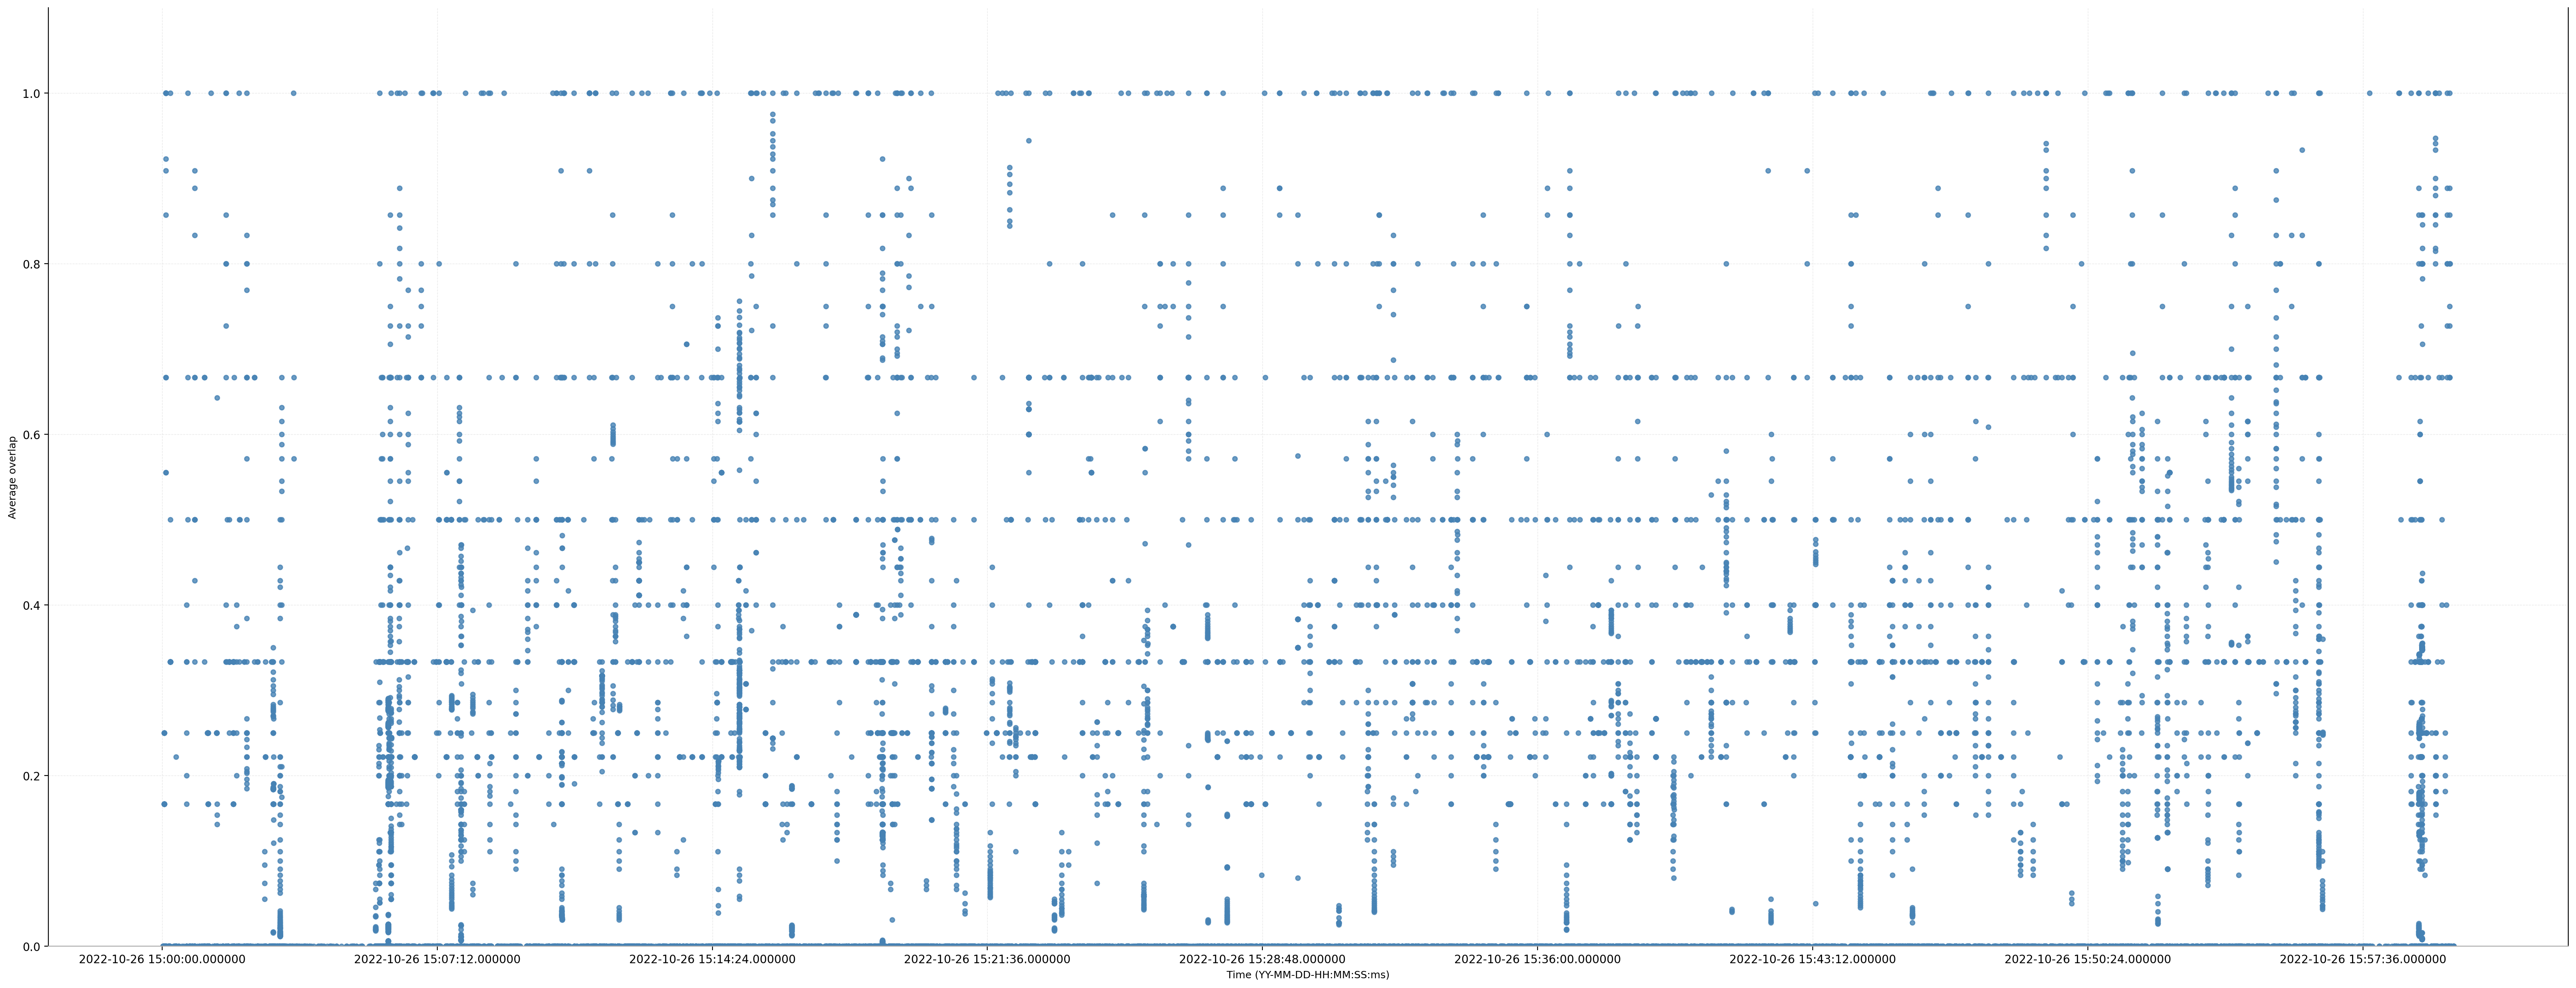
\includegraphics[width=1.45\textwidth, height=\textheight, keepaspectratio]{figures/plots/Scenario-2/G2-overlap.png}
  \caption[Overlap of Packet Success \& Failure with Rolling Time Average]{Scenario-2: Overlap values calculated using a rolling time window of 100ms. The x-axis represents the rolling timestamp values, while the y-axis shows the calculated overlap value. Further details on the calculation can be found in Section \ref{Overlap}.}
  \label{fig:overlap2}
\end{figure}
\FloatBarrier 
\end{landscape}

\section{summary}
This chapter presents an analysis and evaluation of the Minstrel-HT rate control algorithm in wireless networks. A Python-based tool was developed to analyze the extracted data from the Linux kernel trace file, enabling the generation of analytical plots for quantitative analysis. These plots include various aspects to observe. The quantitative calculation and importance of these values are covered in Section~\ref{sec:Analysis and Optimization:Implementation of an Analysis Tool}.

The sub-chapter dedicated to performance evaluation, Section~\ref{sec:Analysis and Optimization:Performance Evaluation}, discusses real-world performance scenarios of the Minstrel-HT algorithm in a desk setup environment, offering a holistic view of its capabilities. The two observed scenarios, Section~\ref{sec:Analysis and Optimization:Performance Evaluation:Scenario1} and Section~\ref{sec:Analysis and Optimization:Performance Evaluation:Scenario2}, are discussed.

By adopting a detailed approach, this study contributes to an understanding of the Minstrel-HT algorithm's performance in real-world settings. The insights gained from this analysis serve as a valuable resource for optimizing wireless network performance and enhancing the reliability of data transmission. The findings presented in this chapter lay the foundation for further research and development in the field of wireless network optimization.
\chapter{Summary and Outlook}
\label{chap:Summary and Outlook}

\section{Summary}

The thesis concludes with a comprehensive analysis of Minstrel-HT rate control algorithm. The three main chapters of the thesis are summarized to highlight the key findings and contributions.

In the first chapter~\ref{chap:introduction}, the concepts of MCS Index and its significance in determining data rates based on channel conditions and supported WiFi standards are explored. The Minstrel-HT algorithm is introduced as an advanced rate control algorithm. In following sub sections The "Rate Group" definition in context of Minstrel-HT been unwrapped \ref{sec:intro:wifiratecontrol:Group creation}, and topics such as rate sampling, MRR chain, and rate statistical calculation are covered in the sub chapters.

The second chapter~\ref{chap:Measurement Tools} focuses on the data collection setup and monitoring information format used in the analysis. It provides a detailed description of the experiment environment, including the diverse positions and orientations of connected devices. By analysing trace files~\cite{SNCX_internal_note} extracted from the Linux kernel, the chapter offers description of each trace line.

In the third chapter (Chapter~\ref{chap:Analysis and Optimization}), a Python-based tool is presented as a means of analysing the collected data and generating analytical plots for quantitative analysis. These plots cover various aspects of network characteristics. Subchapter~\ref{sec:Analysis and Optimization:Implementation of an Analysis Tool} focuses on the calculation of retrieved values from the dataset and describes the importance of each plot for observation. In Subchapter~\ref{sec:Analysis and Optimization:Performance Evaluation}, additional plots are shown.

Overall, the thesis provides a comprehensive analysis of WiFi data transmission, offering insights into modulation, coding schemes, and the performance of the Minstrel-HT rate control algorithm. The Python-based analytical tool and the generated plots contribute to a deeper understanding of the data transmission process, enabling the optimization of wireless network performance and the improvement of data transmission reliability.

The findings presented in this thesis lay the foundation for further research and development in the field of wireless network optimization.

\section{Future Directions}

As the study concludes, there exists potential directions for future research and development in the field of wireless network optimization. These directions aim to enhance the understanding and application of wireless network optimization techniques. The following areas can be explored:

\textbf{Improving the Analytic Tool:} One area for future exploration involves improving the analytical tool used in this study to better visualize and comprehend various aspects of data transmission. This could involve incorporating additional metrics, visual representations, interactive features and enhancing the dynamic capabilities of the Python tool to provide a better understanding of wireless network performance. One of the suggested metrics to observe~\ref{Overlap} is Overlap value.

\textbf{Extending the Scope of Observations:} Expanding the application of the tool to observe and analyse a wider range of scenarios would be a valuable avenue for future research. By capturing diverse network configurations, traffic patterns, and environmental conditions, researchers can gain insights into the robustness and adaptability of optimization algorithms across different real-world settings.

\textbf{Exploring Alternative Optimization Algorithms:} This study focused on a specific optimization algorithm; however, future research can investigate the performance of different algorithms and compare their effectiveness in improving transmission rates. This exploration can lead to a better understanding of algorithmic strengths and weaknesses, enabling the development of more efficient solutions for optimization.

\textbf{Protecting Important Details:} As the analytical tool evolves, it is crucial to ensure that it does not sacrifice essential details that can influence transmission rates. Future research should aim to strike a balance between capturing relevant factors affecting network optimization while still providing a comprehensive overview. This could involve adjusting visualization techniques and data representation methods to maintain a high level of resolution without overwhelming users with too much information.
\chapter{Appendix}
\label{chap:appendix}

%BIBLIOGRAPHY
\addcontentsline{toc}{chapter}{Bibliography}
\bibliographystyle{IEEEtran}
\fancyhead[RE]{\normalfont Bibliography}
\fancyhead[LO]{\normalfont Bibliography}
\bibliography{bibliography/IEEEabrv,bibliography/sample.bib}


%ABBILDUNGSVERZEICHNIS
\addcontentsline{toc}{chapter}{List of Figures}
\listoffigures

%TABELLENVERZEICHNIS
\addcontentsline{toc}{chapter}{List of Tables}
\listoftables



% \backmatter
%\include{cv}

\end{document}
